% Capitolul 11: Analiză spectrală și analiză wavelet
% Analiza avansată a seriilor de timp și previziune -- Programul de master Statistică aplicată și data science, anul I, semestrul 2, Academia de Studii Economice din București
% GENERAT de latex/build_chapter11.py -- modificați generatorul, nu acest fișier.

\newcommand{\coursename}{Analiza avansată a seriilor de timp și previziune}
\def\atslang{ro}
% Preambul comun ATS -- Analiza avansată a seriilor de timp și previziune / Advanced Time Series Analysis and Forecasting
% (Beamer, 16:9). Același design ca MFM, SFM și TSA (copiat din TSA, 5 octombrie 2026). Înainte de % Preambul comun ATS -- Analiza avansată a seriilor de timp și previziune / Advanced Time Series Analysis and Forecasting
% (Beamer, 16:9). Același design ca MFM, SFM și TSA (copiat din TSA, 5 octombrie 2026). Înainte de % Preambul comun ATS -- Analiza avansată a seriilor de timp și previziune / Advanced Time Series Analysis and Forecasting
% (Beamer, 16:9). Același design ca MFM, SFM și TSA (copiat din TSA, 5 octombrie 2026). Înainte de \input{../../latex/preamble} se definește
%   \newcommand{\coursename}{Advanced Time Series Analysis and Forecasting}          (EN)
%   \newcommand{\coursename}{Analiza avansată a seriilor de timp și previziune}       (RO)  și  \def\atslang{ro}
% Fișierele .tex se află în EN/Courses, EN/Seminars, RO/Cursuri, RO/Seminarii (două niveluri sub rădăcină).
% Deck-urile sînt generate de latex/build_chapterN.py / build_seminarN.py (vezi latex/ats_build.py).

\documentclass[9pt, aspectratio=169, t]{beamer}
\providecommand{\coursename}{Advanced Time Series Analysis and Forecasting}

% Ensure content fits on slides
\setbeamersize{text margin left=8mm, text margin right=8mm}
% Smaller institute font (title page)
\setbeamerfont{institute}{size=\footnotesize}

%=============================================================================
% THEME AND STYLE CONFIGURATION
%=============================================================================
\usetheme{default}
% Using default theme for clean header/footer control

% Color Palette (matching Redispatch PDF)
\definecolor{MainBlue}{RGB}{26, 58, 110}
\definecolor{AccentBlue}{RGB}{26, 58, 110}
\definecolor{IDAred}{RGB}{205, 0, 0}
\definecolor{DarkGray}{RGB}{51, 51, 51}
\definecolor{MediumGray}{RGB}{128, 128, 128}
\definecolor{LightGray}{RGB}{248, 248, 248}
\definecolor{VeryLightGray}{RGB}{235, 235, 235}
\definecolor{KeynoteGray}{RGB}{218, 218, 218}
\definecolor{SectionGray}{RGB}{120, 120, 120}
\definecolor{FooterGray}{RGB}{100, 100, 100}
\definecolor{Crimson}{RGB}{220, 53, 69}
\definecolor{Forest}{RGB}{46, 125, 50}
\definecolor{Amber}{RGB}{181, 133, 63}
\definecolor{Orange}{RGB}{230, 126, 34}
\definecolor{Purple}{RGB}{142, 68, 173}

% Gradient background (exact Keynote 315° gradient: white to RGB 218,218,218)
\setbeamertemplate{background}{%
    \begin{tikzpicture}[remember picture, overlay]
        \shade[shading=axis, shading angle=315,
        top color=white, bottom color=KeynoteGray]
        (current page.south west) rectangle (current page.north east);
    \end{tikzpicture}%
}
% Fallback solid color for compatibility
\setbeamercolor{background canvas}{bg=}

\setbeamercolor{palette primary}{bg=MainBlue, fg=white}
\setbeamercolor{palette secondary}{bg=MainBlue!85, fg=white}
\setbeamercolor{palette tertiary}{bg=MainBlue!70, fg=white}
\setbeamercolor{structure}{fg=MainBlue}
\setbeamercolor{title}{fg=IDAred}
\setbeamercolor{frametitle}{fg=IDAred, bg=}
\setbeamercolor{block title}{bg=MainBlue, fg=white}
\setbeamercolor{block body}{bg=VeryLightGray, fg=DarkGray}
\setbeamercolor{block title alerted}{bg=Crimson, fg=white}
\setbeamercolor{block body alerted}{bg=Crimson!8, fg=DarkGray}
\setbeamercolor{block title example}{bg=Forest, fg=white}
\setbeamercolor{block body example}{bg=Forest!8, fg=DarkGray}
\setbeamercolor{item}{fg=MainBlue}

% Footer colors (override Madrid theme blue)
\setbeamercolor{author in head/foot}{fg=FooterGray, bg=}
\setbeamercolor{title in head/foot}{fg=FooterGray, bg=}
\setbeamercolor{date in head/foot}{fg=FooterGray, bg=}
\setbeamercolor{section in head/foot}{fg=FooterGray, bg=}
\setbeamercolor{subsection in head/foot}{fg=FooterGray, bg=}

% Bullet styles (apply everywhere including blocks)
\setbeamertemplate{itemize item}{\color{MainBlue}$\boxdot$}
\setbeamertemplate{itemize subitem}{\color{MainBlue}$\blacktriangleright$}
\setbeamertemplate{itemize subsubitem}{\color{MainBlue}\tiny$\bullet$}
\setbeamertemplate{itemize/enumerate body begin}{\normalsize}
\setbeamertemplate{itemize/enumerate subbody begin}{\normalsize}

% Item spacing - compact style
\setlength{\leftmargini}{10pt}       % Level 1: minimal indent
\setlength{\leftmarginii}{10pt}      % Level 2: minimal additional indent
% Compact list spacing (zero extra space before/after lists in blocks)
\makeatletter
\def\@listi{\leftmargin\leftmargini \topsep 0pt \parsep 0pt \itemsep 0pt}
\def\@listii{\leftmargin\leftmarginii \topsep 0pt \parsep 0pt \itemsep 0pt}
\makeatother

\setbeamertemplate{navigation symbols}{}

%=============================================================================
% CUSTOM HEADLINE
%=============================================================================
\setbeamertemplate{headline}{%
    \vskip10pt%
    \hbox to \paperwidth{%
        \hskip0.5cm%
        {\small\color{FooterGray}\renewcommand{\hyperlink}[2]{##2}\insertsectionhead}%
        \hfill%
        \textcolor{FooterGray}{\small\insertframenumber}%
        \hskip0.5cm%
    }%
    \vskip4pt%
    {\color{FooterGray}\hrule height 0.4pt}%
}

%=============================================================================
% CUSTOM FOOTER
%=============================================================================
\usepackage{fontawesome5}

\setbeamertemplate{footline}{%
    {\color{FooterGray}\hrule height 0.4pt}%
    \vskip4pt%
    \hbox to \paperwidth{%
        \hskip0.5cm%
        \textcolor{FooterGray}{\small\coursename}%
        \hfill%
        \raisebox{-0.1em}{%
            \begin{tikzpicture}[x=0.08em, y=0.08em, line width=0.4pt]
                \draw[FooterGray] (0,3) -- (1,4) -- (2,3.5) -- (3,5) -- (4,4) -- (5,6) -- (6,5.5) -- (7,4) -- (8,5) -- (9,7) -- (10,6) -- (11,5) -- (12,6.5) -- (13,8) -- (14,7) -- (15,6) -- (16,7.5) -- (17,9) -- (18,8) -- (19,7) -- (20,8.5) -- (21,10) -- (22,9) -- (23,8) -- (24,9.5);
            \end{tikzpicture}%
        }%
        \hskip0.5cm%
    }%
    \vskip6pt%
}

%=============================================================================
% PACKAGES
%=============================================================================
\usepackage[utf8]{inputenc}
\DeclareUnicodeCharacter{03B1}{\ensuremath{\alpha}}
\usepackage[T1]{fontenc}
\usepackage{amsmath, amssymb, amsthm}
\usepackage{mathtools}
\usepackage{bm}
\usepackage{tikz}
\usetikzlibrary{arrows.meta, positioning, shapes, calc, decorations.pathreplacing, shadings}
\usepackage{booktabs}
\usepackage{multirow}
\usepackage{array}
\usepackage{graphicx}
\usepackage{animate}
\usepackage{hyperref}
\usepackage{colortbl}
\usepackage{listings}
\lstset{language=Python, basicstyle=\ttfamily\scriptsize, keywordstyle=\color{MainBlue}\bfseries,
  commentstyle=\color{Forest}, stringstyle=\color{Crimson}, breaklines=true,
  frame=none, backgroundcolor=\color{VeryLightGray}, xleftmargin=2mm}
\hypersetup{colorlinks=true, linkcolor=MainBlue, urlcolor=MainBlue}
\graphicspath{{../../logos/}{../../charts/}{../../photos/}}
\usepackage{xcolor}
\hfuzz=2pt  % Suppress tiny overfull warnings (<2pt)
\vfuzz=2pt  % Suppress tiny vertical overfull warnings (<2pt)

%=============================================================================
% QUANTLET COMMANDS
%   \quantlet{<displayed name>}{<url>}       (generic)
%   \atsquantlet{Ch_05}{ATS_ch5_garch}       -> https://github.com/danpele/Advanced-Time-Series/tree/main/Quantlets/Ch_05/ATS_ch5_garch
%   \qlurl{<folder>} is defined per chapter by the generator (Quantlets/Ch_NN/<folder>)
%=============================================================================
\newcommand{\atsrepo}{https://github.com/danpele/Advanced-Time-Series}
\newcommand{\atsqlbase}{https://github.com/danpele/Advanced-Time-Series/tree/main/Quantlets}
\newcommand{\quantlet}[2]{%
    \hfill\href{#2}{%
        \raisebox{-0.15em}{
\includegraphics[height=0.7em]{ql_logo.png}}%
        \textcolor{MainBlue}{\tiny\ #1}%
    }%
}
\newcommand{\atsquantlet}[2]{\quantlet{\detokenize{#2}}{\atsqlbase/#1/#2}}

%=============================================================================
% NOTEBOOKS (Google Colab)
%   \colaburl{notebooks/EN/chapter5_seminar_notebook.ipynb} -> the Colab link of a file in the ATS repo
%   \nb: the chapter notebook (each seminar deck redefines it with \renewcommand)
%=============================================================================
\newcommand{\colaburl}[1]{https://colab.research.google.com/github/danpele/Advanced-Time-Series/blob/main/#1}
\newcommand{\nb}{https://colab.research.google.com/github/danpele/Advanced-Time-Series/tree/main/notebooks/EN}
\newcommand{\nbname}{notebooks/EN}

%=============================================================================
% SLIDE HELPERS (used by the generators; the same as in MFM)
%=============================================================================
% local font size for list bodies (the preamble forces \normalsize)
\newcommand{\itemsize}[1]{\setbeamertemplate{itemize/enumerate body begin}{#1}\setbeamertemplate{itemize/enumerate subbody begin}{#1}}
\newcommand{\intitle}[1]{{\hypersetup{urlcolor=white}#1}}   % white links inside coloured title bars
\newcommand{\imgcap}[1]{{\scriptsize #1}\\[0.5mm]}          % caption under a photo
\newcommand{\imgcredit}[2]{{\tiny\color{FooterGray}\href{#1}{#2}}}   % image credit: source URL, author/licence
\newcommand{\aiprompt}[1]{{\ttfamily\color{MainBlue}#1}}     % a prompt to an AI assistant

%=============================================================================
% SEMINARS: student version by default; the instructor wrapper *_solutions.tex sets \solutionstrue
%=============================================================================
\makeatletter\@ifundefined{ifsolutions}{\expandafter\newif\csname ifsolutions\endcsname}{}\makeatother
\newcommand{\solonly}[1]{\ifsolutions #1\fi}
\newcommand{\propsub}{\ifsolutions\else\framesubtitle{\ifdefined\atslang Rezolvarea se discută la seminar\else Solution discussed in class\fi}\fi}

%=============================================================================
% APPENDIX AND CHAPTER LINKS (latex/appendix_links.py writes the calls; it also re-declares these
% macros before \begin{document}, so the decks compile with or without this preamble block)
%=============================================================================
\providecommand{\atsapplink}[3]{\hypertarget{#2}{}\hyperlink{#1}{\beamergotobutton{#3}}}
\providecommand{\atsappback}[2]{\begin{tikzpicture}[remember picture,overlay]\node[anchor=south east] at ([xshift=-3mm,yshift=7mm]current page.south east){\hyperlink{#1}{\beamerreturnbutton{#2}}};\end{tikzpicture}}
\providecommand{\atschlink}[2]{\href{#1}{#2}}
\providecommand{\atschlinkt}[2]{\href{#1}{\usebeamercolor[fg]{frametitle}#2}}

%=============================================================================
% QUANTINAR COMMAND: link către un curs Quantinar (subiecte avansate)
%=============================================================================
\newcommand{\quantinar}[2]{%
    \href{#2}{%
        \raisebox{-0.15em}{
\includegraphics[height=0.8em]{qr_logo.png}}%
        \textcolor{MainBlue}{\scriptsize\ #1}%
    }%
}

%=============================================================================
% CUSTOM TITLE PAGE
%=============================================================================
\defbeamertemplate*{title page}{hybrid}[1][]
{
    \vspace{0.2cm}
    % Logos row - top header (with clickable links)
    \begin{center}
        \href{https://www.ase.ro}{
\includegraphics[height=1.0cm]{ase_logo.png}}\hspace{0.3cm}%
        \href{https://theida.net}{
\includegraphics[height=1.0cm]{ida_logo.png}}\hspace{0.3cm}%
        \href{https://blockchain-research-center.com}{
\includegraphics[height=1.0cm]{brc_logo.png}}\hspace{0.3cm}%
        \href{https://www.ai4efin.ase.ro}{
\includegraphics[height=1.0cm]{ai4efin_logo.png}}\hspace{0.3cm}%
        \href{https://ipe.ro/new}{
\includegraphics[height=1.0cm]{acad_logo.png}}\hspace{0.3cm}%
        \href{https://www.digital-finance-msca.com}{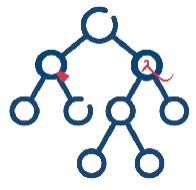
\includegraphics[height=1.0cm]{msca_logo.png}}%
    \end{center}

    \vspace{0.6cm}

    % Main title with Q logos on sides (with clickable links)
    \begin{center}
        \begin{minipage}{0.1\textwidth}
            \centering
            \href{https://quantlet.com}{
\includegraphics[height=1.1cm]{ql_logo.png}}
        \end{minipage}%
        \begin{minipage}{0.78\textwidth}
            \centering
            {\LARGE\bfseries\usebeamercolor[fg]{title}\inserttitle}

            \vspace{0.3cm}

            {\usebeamerfont{subtitle}\usebeamercolor[fg]{title}\insertsubtitle}
        \end{minipage}%
        \begin{minipage}{0.1\textwidth}
            \centering
            \href{https://quantinar.com}{
\includegraphics[height=1.1cm]{qr_logo.png}}
        \end{minipage}
    \end{center}

    \vspace{0.6cm}

    % Authors (left aligned)
    \hspace{0.5cm}{\usebeamerfont{author}\insertauthor}

    \vspace{0.3cm}

    % Institute/Affiliations (left aligned)
    \hspace{0.5cm}\begin{minipage}[t]{0.9\textwidth}
        \raggedright\small\insertinstitute
    \end{minipage}
}

%=============================================================================
% THEOREM ENVIRONMENTS
%=============================================================================
\theoremstyle{definition}
\setbeamertemplate{theorems}[numbered]
\ifdefined\atslang
\newtheorem{defn}{Definiție}
\newtheorem{thm}{Teoremă}
\newtheorem{prop}{Propoziție}
\newtheorem{rmk}{Observație}
\else
\newtheorem{defn}{Definition}
\newtheorem{thm}{Theorem}
\newtheorem{prop}{Proposition}
\newtheorem{rmk}{Remark}
\fi

%=============================================================================
% CENTRED MINIPAGE (no extra vertical space)
%=============================================================================
\newenvironment{cminipage}[1]{%
    \par\noindent\hfill\begin{minipage}{#1}\ignorespaces
}{%
    \end{minipage}\hfill\null\par
}

%=============================================================================
% CUSTOM COMMANDS
%=============================================================================
\newcommand{\E}{\mathbb{E}}
\newcommand{\Var}{\text{Var}}
\newcommand{\Cov}{\text{Cov}}
\newcommand{\Corr}{\text{Corr}}
\newcommand{\R}{\mathbb{R}}
\newcommand{\N}{\mathbb{N}}
\newcommand{\Z}{\mathbb{Z}}
\newcommand{\B}{\mathbf{B}}
\newcommand{\imark}{\textcolor{MainBlue}{\textbullet}}
\newcommand{\RMSE}{\text{RMSE}}
\newcommand{\MAE}{\text{MAE}}
\newcommand{\MAPE}{\text{MAPE}}

% Boldface vector/matrix commands (VAR, VECM, state space)
\newcommand{\bY}{\mathbf{Y}}
\newcommand{\bX}{\mathbf{X}}
\newcommand{\bA}{\mathbf{A}}
\newcommand{\bB}{\mathbf{B}}
\newcommand{\bepsilon}{\boldsymbol{\varepsilon}}
\newcommand{\bSigma}{\boldsymbol{\Sigma}}
\newcommand{\bPhi}{\boldsymbol{\Phi}}
\newcommand{\bGamma}{\boldsymbol{\Gamma}}
\newcommand{\bPi}{\boldsymbol{\Pi}}
\newcommand{\bc}{\mathbf{c}}
\newcommand{\balpha}{\boldsymbol{\alpha}}
\newcommand{\bbeta}{\boldsymbol{\beta}}
\newcommand{\bvarepsilon}{\boldsymbol{\varepsilon}}

% Seminar marks
\newcommand{\correct}{\textcolor{Forest}{\checkmark}}
\newcommand{\incorrect}{\textcolor{Crimson}{\texttimes}}
 se definește
%   \newcommand{\coursename}{Advanced Time Series Analysis and Forecasting}          (EN)
%   \newcommand{\coursename}{Analiza avansată a seriilor de timp și previziune}       (RO)  și  \def\atslang{ro}
% Fișierele .tex se află în EN/Courses, EN/Seminars, RO/Cursuri, RO/Seminarii (două niveluri sub rădăcină).
% Deck-urile sînt generate de latex/build_chapterN.py / build_seminarN.py (vezi latex/ats_build.py).

\documentclass[9pt, aspectratio=169, t]{beamer}
\providecommand{\coursename}{Advanced Time Series Analysis and Forecasting}

% Ensure content fits on slides
\setbeamersize{text margin left=8mm, text margin right=8mm}
% Smaller institute font (title page)
\setbeamerfont{institute}{size=\footnotesize}

%=============================================================================
% THEME AND STYLE CONFIGURATION
%=============================================================================
\usetheme{default}
% Using default theme for clean header/footer control

% Color Palette (matching Redispatch PDF)
\definecolor{MainBlue}{RGB}{26, 58, 110}
\definecolor{AccentBlue}{RGB}{26, 58, 110}
\definecolor{IDAred}{RGB}{205, 0, 0}
\definecolor{DarkGray}{RGB}{51, 51, 51}
\definecolor{MediumGray}{RGB}{128, 128, 128}
\definecolor{LightGray}{RGB}{248, 248, 248}
\definecolor{VeryLightGray}{RGB}{235, 235, 235}
\definecolor{KeynoteGray}{RGB}{218, 218, 218}
\definecolor{SectionGray}{RGB}{120, 120, 120}
\definecolor{FooterGray}{RGB}{100, 100, 100}
\definecolor{Crimson}{RGB}{220, 53, 69}
\definecolor{Forest}{RGB}{46, 125, 50}
\definecolor{Amber}{RGB}{181, 133, 63}
\definecolor{Orange}{RGB}{230, 126, 34}
\definecolor{Purple}{RGB}{142, 68, 173}

% Gradient background (exact Keynote 315° gradient: white to RGB 218,218,218)
\setbeamertemplate{background}{%
    \begin{tikzpicture}[remember picture, overlay]
        \shade[shading=axis, shading angle=315,
        top color=white, bottom color=KeynoteGray]
        (current page.south west) rectangle (current page.north east);
    \end{tikzpicture}%
}
% Fallback solid color for compatibility
\setbeamercolor{background canvas}{bg=}

\setbeamercolor{palette primary}{bg=MainBlue, fg=white}
\setbeamercolor{palette secondary}{bg=MainBlue!85, fg=white}
\setbeamercolor{palette tertiary}{bg=MainBlue!70, fg=white}
\setbeamercolor{structure}{fg=MainBlue}
\setbeamercolor{title}{fg=IDAred}
\setbeamercolor{frametitle}{fg=IDAred, bg=}
\setbeamercolor{block title}{bg=MainBlue, fg=white}
\setbeamercolor{block body}{bg=VeryLightGray, fg=DarkGray}
\setbeamercolor{block title alerted}{bg=Crimson, fg=white}
\setbeamercolor{block body alerted}{bg=Crimson!8, fg=DarkGray}
\setbeamercolor{block title example}{bg=Forest, fg=white}
\setbeamercolor{block body example}{bg=Forest!8, fg=DarkGray}
\setbeamercolor{item}{fg=MainBlue}

% Footer colors (override Madrid theme blue)
\setbeamercolor{author in head/foot}{fg=FooterGray, bg=}
\setbeamercolor{title in head/foot}{fg=FooterGray, bg=}
\setbeamercolor{date in head/foot}{fg=FooterGray, bg=}
\setbeamercolor{section in head/foot}{fg=FooterGray, bg=}
\setbeamercolor{subsection in head/foot}{fg=FooterGray, bg=}

% Bullet styles (apply everywhere including blocks)
\setbeamertemplate{itemize item}{\color{MainBlue}$\boxdot$}
\setbeamertemplate{itemize subitem}{\color{MainBlue}$\blacktriangleright$}
\setbeamertemplate{itemize subsubitem}{\color{MainBlue}\tiny$\bullet$}
\setbeamertemplate{itemize/enumerate body begin}{\normalsize}
\setbeamertemplate{itemize/enumerate subbody begin}{\normalsize}

% Item spacing - compact style
\setlength{\leftmargini}{10pt}       % Level 1: minimal indent
\setlength{\leftmarginii}{10pt}      % Level 2: minimal additional indent
% Compact list spacing (zero extra space before/after lists in blocks)
\makeatletter
\def\@listi{\leftmargin\leftmargini \topsep 0pt \parsep 0pt \itemsep 0pt}
\def\@listii{\leftmargin\leftmarginii \topsep 0pt \parsep 0pt \itemsep 0pt}
\makeatother

\setbeamertemplate{navigation symbols}{}

%=============================================================================
% CUSTOM HEADLINE
%=============================================================================
\setbeamertemplate{headline}{%
    \vskip10pt%
    \hbox to \paperwidth{%
        \hskip0.5cm%
        {\small\color{FooterGray}\renewcommand{\hyperlink}[2]{##2}\insertsectionhead}%
        \hfill%
        \textcolor{FooterGray}{\small\insertframenumber}%
        \hskip0.5cm%
    }%
    \vskip4pt%
    {\color{FooterGray}\hrule height 0.4pt}%
}

%=============================================================================
% CUSTOM FOOTER
%=============================================================================
\usepackage{fontawesome5}

\setbeamertemplate{footline}{%
    {\color{FooterGray}\hrule height 0.4pt}%
    \vskip4pt%
    \hbox to \paperwidth{%
        \hskip0.5cm%
        \textcolor{FooterGray}{\small\coursename}%
        \hfill%
        \raisebox{-0.1em}{%
            \begin{tikzpicture}[x=0.08em, y=0.08em, line width=0.4pt]
                \draw[FooterGray] (0,3) -- (1,4) -- (2,3.5) -- (3,5) -- (4,4) -- (5,6) -- (6,5.5) -- (7,4) -- (8,5) -- (9,7) -- (10,6) -- (11,5) -- (12,6.5) -- (13,8) -- (14,7) -- (15,6) -- (16,7.5) -- (17,9) -- (18,8) -- (19,7) -- (20,8.5) -- (21,10) -- (22,9) -- (23,8) -- (24,9.5);
            \end{tikzpicture}%
        }%
        \hskip0.5cm%
    }%
    \vskip6pt%
}

%=============================================================================
% PACKAGES
%=============================================================================
\usepackage[utf8]{inputenc}
\DeclareUnicodeCharacter{03B1}{\ensuremath{\alpha}}
\usepackage[T1]{fontenc}
\usepackage{amsmath, amssymb, amsthm}
\usepackage{mathtools}
\usepackage{bm}
\usepackage{tikz}
\usetikzlibrary{arrows.meta, positioning, shapes, calc, decorations.pathreplacing, shadings}
\usepackage{booktabs}
\usepackage{multirow}
\usepackage{array}
\usepackage{graphicx}
\usepackage{animate}
\usepackage{hyperref}
\usepackage{colortbl}
\usepackage{listings}
\lstset{language=Python, basicstyle=\ttfamily\scriptsize, keywordstyle=\color{MainBlue}\bfseries,
  commentstyle=\color{Forest}, stringstyle=\color{Crimson}, breaklines=true,
  frame=none, backgroundcolor=\color{VeryLightGray}, xleftmargin=2mm}
\hypersetup{colorlinks=true, linkcolor=MainBlue, urlcolor=MainBlue}
\graphicspath{{../../logos/}{../../charts/}{../../photos/}}
\usepackage{xcolor}
\hfuzz=2pt  % Suppress tiny overfull warnings (<2pt)
\vfuzz=2pt  % Suppress tiny vertical overfull warnings (<2pt)

%=============================================================================
% QUANTLET COMMANDS
%   \quantlet{<displayed name>}{<url>}       (generic)
%   \atsquantlet{Ch_05}{ATS_ch5_garch}       -> https://github.com/danpele/Advanced-Time-Series/tree/main/Quantlets/Ch_05/ATS_ch5_garch
%   \qlurl{<folder>} is defined per chapter by the generator (Quantlets/Ch_NN/<folder>)
%=============================================================================
\newcommand{\atsrepo}{https://github.com/danpele/Advanced-Time-Series}
\newcommand{\atsqlbase}{https://github.com/danpele/Advanced-Time-Series/tree/main/Quantlets}
\newcommand{\quantlet}[2]{%
    \hfill\href{#2}{%
        \raisebox{-0.15em}{
\includegraphics[height=0.7em]{ql_logo.png}}%
        \textcolor{MainBlue}{\tiny\ #1}%
    }%
}
\newcommand{\atsquantlet}[2]{\quantlet{\detokenize{#2}}{\atsqlbase/#1/#2}}

%=============================================================================
% NOTEBOOKS (Google Colab)
%   \colaburl{notebooks/EN/chapter5_seminar_notebook.ipynb} -> the Colab link of a file in the ATS repo
%   \nb: the chapter notebook (each seminar deck redefines it with \renewcommand)
%=============================================================================
\newcommand{\colaburl}[1]{https://colab.research.google.com/github/danpele/Advanced-Time-Series/blob/main/#1}
\newcommand{\nb}{https://colab.research.google.com/github/danpele/Advanced-Time-Series/tree/main/notebooks/EN}
\newcommand{\nbname}{notebooks/EN}

%=============================================================================
% SLIDE HELPERS (used by the generators; the same as in MFM)
%=============================================================================
% local font size for list bodies (the preamble forces \normalsize)
\newcommand{\itemsize}[1]{\setbeamertemplate{itemize/enumerate body begin}{#1}\setbeamertemplate{itemize/enumerate subbody begin}{#1}}
\newcommand{\intitle}[1]{{\hypersetup{urlcolor=white}#1}}   % white links inside coloured title bars
\newcommand{\imgcap}[1]{{\scriptsize #1}\\[0.5mm]}          % caption under a photo
\newcommand{\imgcredit}[2]{{\tiny\color{FooterGray}\href{#1}{#2}}}   % image credit: source URL, author/licence
\newcommand{\aiprompt}[1]{{\ttfamily\color{MainBlue}#1}}     % a prompt to an AI assistant

%=============================================================================
% SEMINARS: student version by default; the instructor wrapper *_solutions.tex sets \solutionstrue
%=============================================================================
\makeatletter\@ifundefined{ifsolutions}{\expandafter\newif\csname ifsolutions\endcsname}{}\makeatother
\newcommand{\solonly}[1]{\ifsolutions #1\fi}
\newcommand{\propsub}{\ifsolutions\else\framesubtitle{\ifdefined\atslang Rezolvarea se discută la seminar\else Solution discussed in class\fi}\fi}

%=============================================================================
% APPENDIX AND CHAPTER LINKS (latex/appendix_links.py writes the calls; it also re-declares these
% macros before \begin{document}, so the decks compile with or without this preamble block)
%=============================================================================
\providecommand{\atsapplink}[3]{\hypertarget{#2}{}\hyperlink{#1}{\beamergotobutton{#3}}}
\providecommand{\atsappback}[2]{\begin{tikzpicture}[remember picture,overlay]\node[anchor=south east] at ([xshift=-3mm,yshift=7mm]current page.south east){\hyperlink{#1}{\beamerreturnbutton{#2}}};\end{tikzpicture}}
\providecommand{\atschlink}[2]{\href{#1}{#2}}
\providecommand{\atschlinkt}[2]{\href{#1}{\usebeamercolor[fg]{frametitle}#2}}

%=============================================================================
% QUANTINAR COMMAND: link către un curs Quantinar (subiecte avansate)
%=============================================================================
\newcommand{\quantinar}[2]{%
    \href{#2}{%
        \raisebox{-0.15em}{
\includegraphics[height=0.8em]{qr_logo.png}}%
        \textcolor{MainBlue}{\scriptsize\ #1}%
    }%
}

%=============================================================================
% CUSTOM TITLE PAGE
%=============================================================================
\defbeamertemplate*{title page}{hybrid}[1][]
{
    \vspace{0.2cm}
    % Logos row - top header (with clickable links)
    \begin{center}
        \href{https://www.ase.ro}{
\includegraphics[height=1.0cm]{ase_logo.png}}\hspace{0.3cm}%
        \href{https://theida.net}{
\includegraphics[height=1.0cm]{ida_logo.png}}\hspace{0.3cm}%
        \href{https://blockchain-research-center.com}{
\includegraphics[height=1.0cm]{brc_logo.png}}\hspace{0.3cm}%
        \href{https://www.ai4efin.ase.ro}{
\includegraphics[height=1.0cm]{ai4efin_logo.png}}\hspace{0.3cm}%
        \href{https://ipe.ro/new}{
\includegraphics[height=1.0cm]{acad_logo.png}}\hspace{0.3cm}%
        \href{https://www.digital-finance-msca.com}{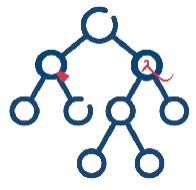
\includegraphics[height=1.0cm]{msca_logo.png}}%
    \end{center}

    \vspace{0.6cm}

    % Main title with Q logos on sides (with clickable links)
    \begin{center}
        \begin{minipage}{0.1\textwidth}
            \centering
            \href{https://quantlet.com}{
\includegraphics[height=1.1cm]{ql_logo.png}}
        \end{minipage}%
        \begin{minipage}{0.78\textwidth}
            \centering
            {\LARGE\bfseries\usebeamercolor[fg]{title}\inserttitle}

            \vspace{0.3cm}

            {\usebeamerfont{subtitle}\usebeamercolor[fg]{title}\insertsubtitle}
        \end{minipage}%
        \begin{minipage}{0.1\textwidth}
            \centering
            \href{https://quantinar.com}{
\includegraphics[height=1.1cm]{qr_logo.png}}
        \end{minipage}
    \end{center}

    \vspace{0.6cm}

    % Authors (left aligned)
    \hspace{0.5cm}{\usebeamerfont{author}\insertauthor}

    \vspace{0.3cm}

    % Institute/Affiliations (left aligned)
    \hspace{0.5cm}\begin{minipage}[t]{0.9\textwidth}
        \raggedright\small\insertinstitute
    \end{minipage}
}

%=============================================================================
% THEOREM ENVIRONMENTS
%=============================================================================
\theoremstyle{definition}
\setbeamertemplate{theorems}[numbered]
\ifdefined\atslang
\newtheorem{defn}{Definiție}
\newtheorem{thm}{Teoremă}
\newtheorem{prop}{Propoziție}
\newtheorem{rmk}{Observație}
\else
\newtheorem{defn}{Definition}
\newtheorem{thm}{Theorem}
\newtheorem{prop}{Proposition}
\newtheorem{rmk}{Remark}
\fi

%=============================================================================
% CENTRED MINIPAGE (no extra vertical space)
%=============================================================================
\newenvironment{cminipage}[1]{%
    \par\noindent\hfill\begin{minipage}{#1}\ignorespaces
}{%
    \end{minipage}\hfill\null\par
}

%=============================================================================
% CUSTOM COMMANDS
%=============================================================================
\newcommand{\E}{\mathbb{E}}
\newcommand{\Var}{\text{Var}}
\newcommand{\Cov}{\text{Cov}}
\newcommand{\Corr}{\text{Corr}}
\newcommand{\R}{\mathbb{R}}
\newcommand{\N}{\mathbb{N}}
\newcommand{\Z}{\mathbb{Z}}
\newcommand{\B}{\mathbf{B}}
\newcommand{\imark}{\textcolor{MainBlue}{\textbullet}}
\newcommand{\RMSE}{\text{RMSE}}
\newcommand{\MAE}{\text{MAE}}
\newcommand{\MAPE}{\text{MAPE}}

% Boldface vector/matrix commands (VAR, VECM, state space)
\newcommand{\bY}{\mathbf{Y}}
\newcommand{\bX}{\mathbf{X}}
\newcommand{\bA}{\mathbf{A}}
\newcommand{\bB}{\mathbf{B}}
\newcommand{\bepsilon}{\boldsymbol{\varepsilon}}
\newcommand{\bSigma}{\boldsymbol{\Sigma}}
\newcommand{\bPhi}{\boldsymbol{\Phi}}
\newcommand{\bGamma}{\boldsymbol{\Gamma}}
\newcommand{\bPi}{\boldsymbol{\Pi}}
\newcommand{\bc}{\mathbf{c}}
\newcommand{\balpha}{\boldsymbol{\alpha}}
\newcommand{\bbeta}{\boldsymbol{\beta}}
\newcommand{\bvarepsilon}{\boldsymbol{\varepsilon}}

% Seminar marks
\newcommand{\correct}{\textcolor{Forest}{\checkmark}}
\newcommand{\incorrect}{\textcolor{Crimson}{\texttimes}}
 se definește
%   \newcommand{\coursename}{Advanced Time Series Analysis and Forecasting}          (EN)
%   \newcommand{\coursename}{Analiza avansată a seriilor de timp și previziune}       (RO)  și  \def\atslang{ro}
% Fișierele .tex se află în EN/Courses, EN/Seminars, RO/Cursuri, RO/Seminarii (două niveluri sub rădăcină).
% Deck-urile sînt generate de latex/build_chapterN.py / build_seminarN.py (vezi latex/ats_build.py).

\documentclass[9pt, aspectratio=169, t]{beamer}
\providecommand{\coursename}{Advanced Time Series Analysis and Forecasting}

% Ensure content fits on slides
\setbeamersize{text margin left=8mm, text margin right=8mm}
% Smaller institute font (title page)
\setbeamerfont{institute}{size=\footnotesize}

%=============================================================================
% THEME AND STYLE CONFIGURATION
%=============================================================================
\usetheme{default}
% Using default theme for clean header/footer control

% Color Palette (matching Redispatch PDF)
\definecolor{MainBlue}{RGB}{26, 58, 110}
\definecolor{AccentBlue}{RGB}{26, 58, 110}
\definecolor{IDAred}{RGB}{205, 0, 0}
\definecolor{DarkGray}{RGB}{51, 51, 51}
\definecolor{MediumGray}{RGB}{128, 128, 128}
\definecolor{LightGray}{RGB}{248, 248, 248}
\definecolor{VeryLightGray}{RGB}{235, 235, 235}
\definecolor{KeynoteGray}{RGB}{218, 218, 218}
\definecolor{SectionGray}{RGB}{120, 120, 120}
\definecolor{FooterGray}{RGB}{100, 100, 100}
\definecolor{Crimson}{RGB}{220, 53, 69}
\definecolor{Forest}{RGB}{46, 125, 50}
\definecolor{Amber}{RGB}{181, 133, 63}
\definecolor{Orange}{RGB}{230, 126, 34}
\definecolor{Purple}{RGB}{142, 68, 173}

% Gradient background (exact Keynote 315° gradient: white to RGB 218,218,218)
\setbeamertemplate{background}{%
    \begin{tikzpicture}[remember picture, overlay]
        \shade[shading=axis, shading angle=315,
        top color=white, bottom color=KeynoteGray]
        (current page.south west) rectangle (current page.north east);
    \end{tikzpicture}%
}
% Fallback solid color for compatibility
\setbeamercolor{background canvas}{bg=}

\setbeamercolor{palette primary}{bg=MainBlue, fg=white}
\setbeamercolor{palette secondary}{bg=MainBlue!85, fg=white}
\setbeamercolor{palette tertiary}{bg=MainBlue!70, fg=white}
\setbeamercolor{structure}{fg=MainBlue}
\setbeamercolor{title}{fg=IDAred}
\setbeamercolor{frametitle}{fg=IDAred, bg=}
\setbeamercolor{block title}{bg=MainBlue, fg=white}
\setbeamercolor{block body}{bg=VeryLightGray, fg=DarkGray}
\setbeamercolor{block title alerted}{bg=Crimson, fg=white}
\setbeamercolor{block body alerted}{bg=Crimson!8, fg=DarkGray}
\setbeamercolor{block title example}{bg=Forest, fg=white}
\setbeamercolor{block body example}{bg=Forest!8, fg=DarkGray}
\setbeamercolor{item}{fg=MainBlue}

% Footer colors (override Madrid theme blue)
\setbeamercolor{author in head/foot}{fg=FooterGray, bg=}
\setbeamercolor{title in head/foot}{fg=FooterGray, bg=}
\setbeamercolor{date in head/foot}{fg=FooterGray, bg=}
\setbeamercolor{section in head/foot}{fg=FooterGray, bg=}
\setbeamercolor{subsection in head/foot}{fg=FooterGray, bg=}

% Bullet styles (apply everywhere including blocks)
\setbeamertemplate{itemize item}{\color{MainBlue}$\boxdot$}
\setbeamertemplate{itemize subitem}{\color{MainBlue}$\blacktriangleright$}
\setbeamertemplate{itemize subsubitem}{\color{MainBlue}\tiny$\bullet$}
\setbeamertemplate{itemize/enumerate body begin}{\normalsize}
\setbeamertemplate{itemize/enumerate subbody begin}{\normalsize}

% Item spacing - compact style
\setlength{\leftmargini}{10pt}       % Level 1: minimal indent
\setlength{\leftmarginii}{10pt}      % Level 2: minimal additional indent
% Compact list spacing (zero extra space before/after lists in blocks)
\makeatletter
\def\@listi{\leftmargin\leftmargini \topsep 0pt \parsep 0pt \itemsep 0pt}
\def\@listii{\leftmargin\leftmarginii \topsep 0pt \parsep 0pt \itemsep 0pt}
\makeatother

\setbeamertemplate{navigation symbols}{}

%=============================================================================
% CUSTOM HEADLINE
%=============================================================================
\setbeamertemplate{headline}{%
    \vskip10pt%
    \hbox to \paperwidth{%
        \hskip0.5cm%
        {\small\color{FooterGray}\renewcommand{\hyperlink}[2]{##2}\insertsectionhead}%
        \hfill%
        \textcolor{FooterGray}{\small\insertframenumber}%
        \hskip0.5cm%
    }%
    \vskip4pt%
    {\color{FooterGray}\hrule height 0.4pt}%
}

%=============================================================================
% CUSTOM FOOTER
%=============================================================================
\usepackage{fontawesome5}

\setbeamertemplate{footline}{%
    {\color{FooterGray}\hrule height 0.4pt}%
    \vskip4pt%
    \hbox to \paperwidth{%
        \hskip0.5cm%
        \textcolor{FooterGray}{\small\coursename}%
        \hfill%
        \raisebox{-0.1em}{%
            \begin{tikzpicture}[x=0.08em, y=0.08em, line width=0.4pt]
                \draw[FooterGray] (0,3) -- (1,4) -- (2,3.5) -- (3,5) -- (4,4) -- (5,6) -- (6,5.5) -- (7,4) -- (8,5) -- (9,7) -- (10,6) -- (11,5) -- (12,6.5) -- (13,8) -- (14,7) -- (15,6) -- (16,7.5) -- (17,9) -- (18,8) -- (19,7) -- (20,8.5) -- (21,10) -- (22,9) -- (23,8) -- (24,9.5);
            \end{tikzpicture}%
        }%
        \hskip0.5cm%
    }%
    \vskip6pt%
}

%=============================================================================
% PACKAGES
%=============================================================================
\usepackage[utf8]{inputenc}
\DeclareUnicodeCharacter{03B1}{\ensuremath{\alpha}}
\usepackage[T1]{fontenc}
\usepackage{amsmath, amssymb, amsthm}
\usepackage{mathtools}
\usepackage{bm}
\usepackage{tikz}
\usetikzlibrary{arrows.meta, positioning, shapes, calc, decorations.pathreplacing, shadings}
\usepackage{booktabs}
\usepackage{multirow}
\usepackage{array}
\usepackage{graphicx}
\usepackage{animate}
\usepackage{hyperref}
\usepackage{colortbl}
\usepackage{listings}
\lstset{language=Python, basicstyle=\ttfamily\scriptsize, keywordstyle=\color{MainBlue}\bfseries,
  commentstyle=\color{Forest}, stringstyle=\color{Crimson}, breaklines=true,
  frame=none, backgroundcolor=\color{VeryLightGray}, xleftmargin=2mm}
\hypersetup{colorlinks=true, linkcolor=MainBlue, urlcolor=MainBlue}
\graphicspath{{../../logos/}{../../charts/}{../../photos/}}
\usepackage{xcolor}
\hfuzz=2pt  % Suppress tiny overfull warnings (<2pt)
\vfuzz=2pt  % Suppress tiny vertical overfull warnings (<2pt)

%=============================================================================
% QUANTLET COMMANDS
%   \quantlet{<displayed name>}{<url>}       (generic)
%   \atsquantlet{Ch_05}{ATS_ch5_garch}       -> https://github.com/danpele/Advanced-Time-Series/tree/main/Quantlets/Ch_05/ATS_ch5_garch
%   \qlurl{<folder>} is defined per chapter by the generator (Quantlets/Ch_NN/<folder>)
%=============================================================================
\newcommand{\atsrepo}{https://github.com/danpele/Advanced-Time-Series}
\newcommand{\atsqlbase}{https://github.com/danpele/Advanced-Time-Series/tree/main/Quantlets}
\newcommand{\quantlet}[2]{%
    \hfill\href{#2}{%
        \raisebox{-0.15em}{
\includegraphics[height=0.7em]{ql_logo.png}}%
        \textcolor{MainBlue}{\tiny\ #1}%
    }%
}
\newcommand{\atsquantlet}[2]{\quantlet{\detokenize{#2}}{\atsqlbase/#1/#2}}

%=============================================================================
% NOTEBOOKS (Google Colab)
%   \colaburl{notebooks/EN/chapter5_seminar_notebook.ipynb} -> the Colab link of a file in the ATS repo
%   \nb: the chapter notebook (each seminar deck redefines it with \renewcommand)
%=============================================================================
\newcommand{\colaburl}[1]{https://colab.research.google.com/github/danpele/Advanced-Time-Series/blob/main/#1}
\newcommand{\nb}{https://colab.research.google.com/github/danpele/Advanced-Time-Series/tree/main/notebooks/EN}
\newcommand{\nbname}{notebooks/EN}

%=============================================================================
% SLIDE HELPERS (used by the generators; the same as in MFM)
%=============================================================================
% local font size for list bodies (the preamble forces \normalsize)
\newcommand{\itemsize}[1]{\setbeamertemplate{itemize/enumerate body begin}{#1}\setbeamertemplate{itemize/enumerate subbody begin}{#1}}
\newcommand{\intitle}[1]{{\hypersetup{urlcolor=white}#1}}   % white links inside coloured title bars
\newcommand{\imgcap}[1]{{\scriptsize #1}\\[0.5mm]}          % caption under a photo
\newcommand{\imgcredit}[2]{{\tiny\color{FooterGray}\href{#1}{#2}}}   % image credit: source URL, author/licence
\newcommand{\aiprompt}[1]{{\ttfamily\color{MainBlue}#1}}     % a prompt to an AI assistant

%=============================================================================
% SEMINARS: student version by default; the instructor wrapper *_solutions.tex sets \solutionstrue
%=============================================================================
\makeatletter\@ifundefined{ifsolutions}{\expandafter\newif\csname ifsolutions\endcsname}{}\makeatother
\newcommand{\solonly}[1]{\ifsolutions #1\fi}
\newcommand{\propsub}{\ifsolutions\else\framesubtitle{\ifdefined\atslang Rezolvarea se discută la seminar\else Solution discussed in class\fi}\fi}

%=============================================================================
% APPENDIX AND CHAPTER LINKS (latex/appendix_links.py writes the calls; it also re-declares these
% macros before \begin{document}, so the decks compile with or without this preamble block)
%=============================================================================
\providecommand{\atsapplink}[3]{\hypertarget{#2}{}\hyperlink{#1}{\beamergotobutton{#3}}}
\providecommand{\atsappback}[2]{\begin{tikzpicture}[remember picture,overlay]\node[anchor=south east] at ([xshift=-3mm,yshift=7mm]current page.south east){\hyperlink{#1}{\beamerreturnbutton{#2}}};\end{tikzpicture}}
\providecommand{\atschlink}[2]{\href{#1}{#2}}
\providecommand{\atschlinkt}[2]{\href{#1}{\usebeamercolor[fg]{frametitle}#2}}

%=============================================================================
% QUANTINAR COMMAND: link către un curs Quantinar (subiecte avansate)
%=============================================================================
\newcommand{\quantinar}[2]{%
    \href{#2}{%
        \raisebox{-0.15em}{
\includegraphics[height=0.8em]{qr_logo.png}}%
        \textcolor{MainBlue}{\scriptsize\ #1}%
    }%
}

%=============================================================================
% CUSTOM TITLE PAGE
%=============================================================================
\defbeamertemplate*{title page}{hybrid}[1][]
{
    \vspace{0.2cm}
    % Logos row - top header (with clickable links)
    \begin{center}
        \href{https://www.ase.ro}{
\includegraphics[height=1.0cm]{ase_logo.png}}\hspace{0.3cm}%
        \href{https://theida.net}{
\includegraphics[height=1.0cm]{ida_logo.png}}\hspace{0.3cm}%
        \href{https://blockchain-research-center.com}{
\includegraphics[height=1.0cm]{brc_logo.png}}\hspace{0.3cm}%
        \href{https://www.ai4efin.ase.ro}{
\includegraphics[height=1.0cm]{ai4efin_logo.png}}\hspace{0.3cm}%
        \href{https://ipe.ro/new}{
\includegraphics[height=1.0cm]{acad_logo.png}}\hspace{0.3cm}%
        \href{https://www.digital-finance-msca.com}{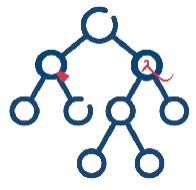
\includegraphics[height=1.0cm]{msca_logo.png}}%
    \end{center}

    \vspace{0.6cm}

    % Main title with Q logos on sides (with clickable links)
    \begin{center}
        \begin{minipage}{0.1\textwidth}
            \centering
            \href{https://quantlet.com}{
\includegraphics[height=1.1cm]{ql_logo.png}}
        \end{minipage}%
        \begin{minipage}{0.78\textwidth}
            \centering
            {\LARGE\bfseries\usebeamercolor[fg]{title}\inserttitle}

            \vspace{0.3cm}

            {\usebeamerfont{subtitle}\usebeamercolor[fg]{title}\insertsubtitle}
        \end{minipage}%
        \begin{minipage}{0.1\textwidth}
            \centering
            \href{https://quantinar.com}{
\includegraphics[height=1.1cm]{qr_logo.png}}
        \end{minipage}
    \end{center}

    \vspace{0.6cm}

    % Authors (left aligned)
    \hspace{0.5cm}{\usebeamerfont{author}\insertauthor}

    \vspace{0.3cm}

    % Institute/Affiliations (left aligned)
    \hspace{0.5cm}\begin{minipage}[t]{0.9\textwidth}
        \raggedright\small\insertinstitute
    \end{minipage}
}

%=============================================================================
% THEOREM ENVIRONMENTS
%=============================================================================
\theoremstyle{definition}
\setbeamertemplate{theorems}[numbered]
\ifdefined\atslang
\newtheorem{defn}{Definiție}
\newtheorem{thm}{Teoremă}
\newtheorem{prop}{Propoziție}
\newtheorem{rmk}{Observație}
\else
\newtheorem{defn}{Definition}
\newtheorem{thm}{Theorem}
\newtheorem{prop}{Proposition}
\newtheorem{rmk}{Remark}
\fi

%=============================================================================
% CENTRED MINIPAGE (no extra vertical space)
%=============================================================================
\newenvironment{cminipage}[1]{%
    \par\noindent\hfill\begin{minipage}{#1}\ignorespaces
}{%
    \end{minipage}\hfill\null\par
}

%=============================================================================
% CUSTOM COMMANDS
%=============================================================================
\newcommand{\E}{\mathbb{E}}
\newcommand{\Var}{\text{Var}}
\newcommand{\Cov}{\text{Cov}}
\newcommand{\Corr}{\text{Corr}}
\newcommand{\R}{\mathbb{R}}
\newcommand{\N}{\mathbb{N}}
\newcommand{\Z}{\mathbb{Z}}
\newcommand{\B}{\mathbf{B}}
\newcommand{\imark}{\textcolor{MainBlue}{\textbullet}}
\newcommand{\RMSE}{\text{RMSE}}
\newcommand{\MAE}{\text{MAE}}
\newcommand{\MAPE}{\text{MAPE}}

% Boldface vector/matrix commands (VAR, VECM, state space)
\newcommand{\bY}{\mathbf{Y}}
\newcommand{\bX}{\mathbf{X}}
\newcommand{\bA}{\mathbf{A}}
\newcommand{\bB}{\mathbf{B}}
\newcommand{\bepsilon}{\boldsymbol{\varepsilon}}
\newcommand{\bSigma}{\boldsymbol{\Sigma}}
\newcommand{\bPhi}{\boldsymbol{\Phi}}
\newcommand{\bGamma}{\boldsymbol{\Gamma}}
\newcommand{\bPi}{\boldsymbol{\Pi}}
\newcommand{\bc}{\mathbf{c}}
\newcommand{\balpha}{\boldsymbol{\alpha}}
\newcommand{\bbeta}{\boldsymbol{\beta}}
\newcommand{\bvarepsilon}{\boldsymbol{\varepsilon}}

% Seminar marks
\newcommand{\correct}{\textcolor{Forest}{\checkmark}}
\newcommand{\incorrect}{\textcolor{Crimson}{\texttimes}}


\newcommand{\qlurl}[1]{https://github.com/danpele/Advanced-Time-Series/tree/main/Quantlets/Ch_11/#1}

% Clickable citations (DOIs verified via Crossref)
\newcommand{\refACS}{\href{https://doi.org/10.1111/joes.12012}{Aguiar-Conraria și Soares (2014)}}
\newcommand{\refAAS}{\href{https://doi.org/10.1016/j.physa.2008.01.063}{Aguiar-Conraria, Azevedo și Soares (2008)}}
\newcommand{\refAnd}{\href{https://doi.org/10.2307/2938229}{Andrews (1991)}}
\newcommand{\refBK}{\href{https://doi.org/10.1162/003465399558454}{Baxter și King (1999)}}
\newcommand{\refBC}{\href{https://doi.org/10.1016/j.jeconom.2005.02.004}{Breitung și Candelon (2006)}}
\newcommand{\refBD}{\href{https://doi.org/10.1007/978-1-4419-0320-4}{Brockwell și Davis (1991)}}
\newcommand{\refCF}{\href{https://doi.org/10.1111/1468-2354.t01-1-00076}{Christiano și Fitzgerald (2003)}}
\newcommand{\refCN}{\href{https://doi.org/10.1016/0165-1889(93)00781-X}{Cogley și Nason (1995)}}
\newcommand{\refCFR}{\href{https://doi.org/10.1162/00346530151143770}{Croux, Forni și Reichlin (2001)}}
\newcommand{\refCro}{\href{https://doi.org/10.1111/j.1467-6419.2006.00502.x}{Crowley (2007)}}
\newcommand{\refDah}{\href{https://doi.org/10.1214/aos/1034276620}{Dahlhaus (1997)}}
\newcommand{\refDau}{\href{https://doi.org/10.1002/cpa.3160410705}{Daubechies (1988)}}
\newcommand{\refFK}{\href{https://doi.org/10.1016/j.jce.2006.06.007}{Fidrmuc și Korhonen (2006)}}
\newcommand{\refFR}{\href{https://doi.org/10.1111/0022-1082.00494}{Forbes și Rigobon (2002)}}
\newcommand{\refGSW}{\href{https://doi.org/10.1016/j.jimonfin.2004.10.003}{Gençay, Selçuk și Whitcher (2005)}}
\newcommand{\refGSWb}{\href{https://doi.org/10.1016/B978-012279670-8.50010-0}{Gençay, Selçuk și Whitcher (2002)}}
\newcommand{\refGew}{\href{https://doi.org/10.1080/01621459.1982.10477803}{Geweke (1982)}}
\newcommand{\refGra}{\href{https://doi.org/10.2307/1909859}{Granger (1966)}}
\newcommand{\refGMJ}{\href{https://doi.org/10.5194/npg-11-561-2004}{Grinsted, Moore și Jevrejeva (2004)}}
\newcommand{\refGM}{\href{https://doi.org/10.1137/0515056}{Grossmann și Morlet (1984)}}
\newcommand{\refHam}{\href{https://doi.org/10.1162/rest_a_00706}{Hamilton (2018)}}
\newcommand{\refHPa}{\href{https://doi.org/10.1016/S0304-3932(01)00108-8}{Harding și Pagan (2002)}}
\newcommand{\refHP}{\href{https://doi.org/10.2307/2953682}{Hodrick și Prescott (1997)}}
\newcommand{\refHur}{\href{https://doi.org/10.1080/01621459.1985.10478207}{Hurvich (1985)}}
\newcommand{\refKP}{\href{https://doi.org/10.1111/j.1468-2354.2009.00568.x}{Kilian și Park (2009)}}
\newcommand{\refLLW}{\href{https://doi.org/10.1175/2007JTECHO511.1}{Liu, Liang și Weisberg (2007)}}
\newcommand{\refMal}{\href{https://doi.org/10.1109/34.192463}{Mallat (1989)}}
\newcommand{\refMK}{\href{https://doi.org/10.5194/npg-11-505-2004}{Maraun și Kurths (2004)}}
\newcommand{\refPar}{\href{https://doi.org/10.1080/00401706.1961.10489939}{Parzen (1961)}}
\newcommand{\refPer}{\href{https://doi.org/10.1093/biomet/82.3.619}{Percival (1995)}}
\newcommand{\refPWa}{\href{https://doi.org/10.1017/CBO9780511622762}{Percival și Walden (1993)}}
\newcommand{\refPWb}{\href{https://doi.org/10.1017/CBO9780511841040}{Percival și Walden (2000)}}
\newcommand{\refPet}{\href{https://doi.org/10.1016/j.ijforecast.2021.11.001}{Petropoulos et al.\ (2022)}}
\newcommand{\refPS}{\href{https://doi.org/10.1111/iere.12495}{Phillips și Shi (2021)}}
\newcommand{\refPri}{\href{https://doi.org/10.1111/j.2517-6161.1965.tb01488.x}{Priestley (1965)}}
\newcommand{\refQW}{\href{https://doi.org/10.1080/07350015.2020.1784747}{Quast și Wolters (2022)}}
\newcommand{\refRU}{\href{https://doi.org/10.1162/003465302317411604}{Ravn și Uhlig (2002)}}
\newcommand{\refRS}{\href{https://doi.org/10.1109/78.365298}{Riedel și Sidorenko (1995)}}
\newcommand{\refRN}{\href{https://doi.org/10.1016/j.jempfin.2009.02.002}{Rua și Nunes (2009)}}
\newcommand{\refSch}{\href{https://doi.org/10.5194/npg-23-45-2016}{Schulte (2016)}}
\newcommand{\refSS}{\href{https://doi.org/10.1007/978-3-319-52452-8}{Shumway și Stoffer (2017)}}
\newcommand{\refTho}{\href{https://doi.org/10.1109/PROC.1982.12433}{Thomson (1982)}}
\newcommand{\refTC}{\href{https://doi.org/10.1175/1520-0477(1998)079\%3C0061:APGTWA\%3E2.0.CO;2}{Torrence și Compo (1998)}}
\newcommand{\refTW}{\href{https://doi.org/10.1175/1520-0442(1999)012\%3C2679:ICITEM\%3E2.0.CO;2}{Torrence și Webster (1999)}}
\newcommand{\refVB}{\href{https://doi.org/10.1016/j.eneco.2011.10.007}{Vacha și Barunik (2012)}}
\newcommand{\refVG}{\href{https://doi.org/10.1016/0167-2789(89)90077-8}{Vautard și Ghil (1989)}}
\newcommand{\refWel}{\href{https://doi.org/10.1109/TAU.1967.1161901}{Welch (1967)}}
\newcommand{\refWGP}{\href{https://doi.org/10.1029/2000JD900110}{Whitcher, Guttorp și Percival (2000)}}

\title[Analiza avansată a seriilor de timp și previziune]{Analiza avansată a seriilor de timp și previziune}
\subtitle{Capitolul 11: Analiză spectrală și analiză wavelet}
\author[D.T. Pele]{Daniel Traian PELE}
\institute{Academia de Studii Economice din București\\
IDA Institute Digital Assets\\
Blockchain Research Center\\
AI4EFin Artificial Intelligence for Energy Finance\\
Academia Română, Institutul de Prognoză Economică\\
MSCA Digital Finance}
\date{}

%=============================================================================
\providecommand{\atsapplink}[3]{\hypertarget{#2}{}\hyperlink{#1}{\beamergotobutton{#3}}}  % APPLINKS-MACROS
\providecommand{\atsappback}[2]{\begin{tikzpicture}[remember picture,overlay]\node[anchor=south east] at ([xshift=-3mm,yshift=7mm]current page.south east){\hyperlink{#1}{\beamerreturnbutton{#2}}};\end{tikzpicture}}  % APPLINKS-MACROS
\providecommand{\atschlink}[2]{\href{#1}{#2}}  % APPLINKS-MACROS
\providecommand{\atschlinkt}[2]{\href{#1}{\usebeamercolor[fg]{frametitle}#2}}  % APPLINKS-MACROS
\begin{document}
%=============================================================================

{
\setbeamertemplate{headline}{}
\setbeamertemplate{footline}{}
\begin{frame}[noframenumbering]
    \titlepage
\end{frame}
}
% BEGIN-ACRONYMS (generat de latex/acronyms.py; nu editati manual)
\begin{frame}{Acronime folosite în acest material (1/2)}
\setbeamertemplate{itemize/enumerate body begin}{\tiny}
\begin{columns}[T]
\begin{column}{0.49\textwidth}
\begin{itemize}\setlength{\itemsep}{0pt}
    \item \textbf{AI}: Artificial Intelligence (inteligență artificială)
    \item \textbf{AIC}: Akaike Information Criterion (criteriul informațional Akaike)
    \item \textbf{AR}: AutoRegressive (model); in event studies: Abnormal Return (model autoregresiv; în studiile de eveniment: randament anormal)
    \item \textbf{ARMA}: AutoRegressive Moving Average (model) — model autoregresiv cu medie mobilă
    \item \textbf{ATS}: Advanced Time Series Analysis and Forecasting (Analiza avansată a seriilor de timp și previziune, cursul de master)
    \item \textbf{BC}: Breitung–Candelon (frequency-domain causality test) — testul de cauzalitate în domeniul frecvenței Breitung–Candelon
    \item \textbf{BET}: Bucharest Exchange Trading (index) — indicele de referință al Bursei de Valori București
    \item \textbf{BK}: Baxter–King (band-pass filter) — filtrul trece-bandă Baxter–King
    \item \textbf{BUX}: Budapesti Értéktőzsde index (indicele Bursei din Budapesta)
    \item \textbf{CF}: Christiano–Fitzgerald (band-pass filter) — filtrul trece-bandă Christiano–Fitzgerald
    \item \textbf{CFR}: Croux, Forni and Reichlin (2001) — Croux, Forni și Reichlin (2001)
    \item \textbf{COI}: Cone Of Influence (of a wavelet transform) — conul de influență al transformatei wavelet
    \item \textbf{CWT}: Continuous Wavelet Transform (transformata wavelet continuă)
\end{itemize}
\end{column}
\begin{column}{0.49\textwidth}
\begin{itemize}\setlength{\itemsep}{0pt}
    \item \textbf{DCC-GARCH}: Dynamic Conditional Correlation GARCH (model GARCH cu corelație condiționată dinamică)
    \item \textbf{DFT}: Discrete Fourier Transform (transformata Fourier discretă)
    \item \textbf{DPSS}: Discrete Prolate Spheroidal Sequences (Slepian tapers) — șiruri sferoidale prolate discrete (taper-ele Slepian)
    \item \textbf{DWT}: Discrete Wavelet Transform (transformata wavelet discretă)
    \item \textbf{EODHD}: EOD Historical Data (market-data provider) — furnizor de date de piață
    \item \textbf{FFT}: Fast Fourier Transform (transformata Fourier rapidă)
    \item \textbf{FRED}: Federal Reserve Economic Data (baza de date economice a Rezervei Federale din St. Louis)
    \item \textbf{GARCH}: Generalised AutoRegressive Conditional Heteroskedasticity (heteroscedasticitate condiționată autoregresivă generalizată)
    \item \textbf{HAC}: Heteroskedasticity and Autocorrelation Consistent (standard errors) — erori standard robuste la heteroscedasticitate și autocorelație
    \item \textbf{HICP}: Harmonised Index of Consumer Prices (indicele armonizat al prețurilor de consum (IAPC))
    \item \textbf{HP}: Hodrick–Prescott (filter) — filtrul Hodrick–Prescott
    \item \textbf{LA}: Least Asymmetric (Daubechies wavelet filter) — filtrul wavelet Daubechies cel mai puțin asimetric
    \item \textbf{LLM}: Large Language Model (model lingvistic de mari dimensiuni)
\end{itemize}
\end{column}
\end{columns}
\end{frame}
\begin{frame}{Acronime folosite în acest material (2/2)}
\setbeamertemplate{itemize/enumerate body begin}{\tiny}
\begin{columns}[T]
\begin{column}{0.49\textwidth}
\begin{itemize}\setlength{\itemsep}{0pt}
    \item \textbf{MODWT}: Maximal Overlap Discrete Wavelet Transform (transformata wavelet discretă cu suprapunere maximă)
    \item \textbf{MRA}: MultiResolution Analysis (analiza multirezoluție)
    \item \textbf{MSE}: Mean Squared Error (eroarea pătratică medie)
    \item \textbf{PIB}: Produsul intern brut
    \item \textbf{PX}: Prague Stock Exchange index (index Burzy cenných papírů Praha) — indicele Bursei din Praga
    \item \textbf{QS}: Quadratic Spectral (kernel) — nucleul spectral pătratic
    \item \textbf{RMSE}: Root Mean Squared Error (rădăcina erorii pătratice medii)
    \item \textbf{SSA}: Singular Spectrum Analysis (analiza spectrului singular)
    \item \textbf{SVD}: Singular Value Decomposition (descompunerea valorilor singulare)
    \item \textbf{TSA}: Time Series Analysis (Serii de timp, cursul de licență)
    \item \textbf{US}: United States (Statele Unite ale Americii)
    \item \textbf{VAR}: Vector AutoRegression (model vector autoregresiv)
    \item \textbf{VARMA}: Vector AutoRegressive Moving Average (model) — model vectorial autoregresiv cu medie mobilă
\end{itemize}
\end{column}
\begin{column}{0.49\textwidth}
\begin{itemize}\setlength{\itemsep}{0pt}
    \item \textbf{WIG20}: Warszawski Indeks Giełdowy 20 (indicele celor mai mari 20 de companii de la Bursa din Varșovia)
\end{itemize}
\end{column}
\end{columns}
\end{frame}
% END-ACRONYMS

\begin{frame}{Întrebarea de azi și traseul}
\itemsize{\small}
\begin{itemize}
    \item \textbf{Întrebarea}: cum se distribuie pe frecvențe varianța unei serii de timp și co-mișcarea a două serii și cum se schimbă această distribuție în timp?
    \begin{itemize}
        \item ciclurile de lungimi diferite răspund unor întrebări economice diferite: ciclul economic, sezonalitatea, reacția piețelor într-o săptămînă
    \end{itemize}
    \item \textbf{Traseul} capitolului
    \begin{itemize}
        \item reprezentarea spectrală; teoria estimării: consistență, lățime de bandă, multitaper
        \item două serii: coerență, fază, corelație dinamică, cauzalitate în domeniul frecvenței
        \item filtre trece-bandă și critica lui Hamilton la adresa filtrului HP; România și zona euro
        \item spectre evolutive; wavelets: MODWT, varianța și corelația pe scale, coerența wavelet
    \end{itemize}
    \item Pornim de la \atschlink{https://danpele.github.io/Time-Series-Analysis/RO/Cursuri/capitol12_analiza_spectrala.pdf}{TSA, Capitolul 12} (periodogramă, netezire, testul lui Fisher, coerență), de la \atschlink{https://danpele.github.io/Advanced-Time-Series/RO/Cursuri/capitol6_modele_spatiul_starilor_filtrare_bayesiana.pdf}{Capitolul 6} (spațiul stărilor) și de la \atschlink{https://danpele.github.io/Advanced-Time-Series/RO/Cursuri/capitol10_memorie_lunga_rough_volatility.pdf}{Capitolul 10} (polul spectral al memoriei lungi); Seminarul 11 are loc înaintea acestui curs
\end{itemize}
\end{frame}

\begin{frame}{Rezultatele învățării}
\itemsize{\small}
\begin{itemize}
    \item Enunțați reprezentarea spectrală a unui proces staționar și derivați spectrul unui proces filtrat
    \item Derivați deplasarea și varianța estimatorilor cu fereastră de decalaje, alegeți lățimea de bandă și construiți estimări multitaper cu benzi de încredere valide
    \item Estimați și testați coerența, faza, cîștigul și corelația dinamică și testați cauzalitatea Granger la o frecvență dată
    \item Evaluați filtrele de tendință și ciclu prin funcția lor de cîștig și măsurați sincronizarea ciclurilor economice
    \item Descompuneți varianța și corelația pe scale prin MODWT și testați coerența wavelet prin Monte Carlo
\end{itemize}
\end{frame}

\begin{frame}{Bibliografie, date și instrumente}
\itemsize{\small}
\begin{itemize}
    \item Teoria și estimarea spectrală: \refBD; \refPWa; \refSS; \refTho
    \begin{itemize}
        \item Wavelets: \refPWb; \refTC; \refGMJ; \refACS
        \item Ciclul economic: \refBK; \refCF; \refHam; \refCFR
        \item Sinteză despre practica prognozei: \refPet
    \end{itemize}
    \item Quantlet-urile Python ale capitolului: \href{https://github.com/danpele/Advanced-Time-Series/tree/main/Quantlets/Ch_11}{Quantlets/Ch\_11}
    \begin{itemize}
        \item spectre, multitaper, spectre încrucișate, Geweke și Breitung--Candelon, filtre, MODWT, transformata Morlet și coerența wavelet scrise în \texttt{numpy}/\texttt{scipy}; \texttt{PyWavelets} furnizează filtrele wavelet
    \end{itemize}
    \item Notebook-ul cursului: \href{\colaburl{notebooks/EN/chapter11_lecture_notebook.ipynb}}{deschideți în Google Colab}
\end{itemize}
\end{frame}

\begin{frame}{Datele folosite în acest capitol}
\itemsize{\footnotesize}
\begin{center}
\scriptsize
\begin{tabular}{>{\raggedright\arraybackslash}p{3.6cm}>{\raggedright\arraybackslash}p{5.0cm}>{\raggedright\arraybackslash}p{3.4cm}}
\toprule
\textbf{Seria} & \textbf{Sursa} & \textbf{Eșantionul} \\
\midrule
PIB real: România, zona euro, Polonia, Ungaria, Cehia & Eurostat, volume înlănțuite, ajustate sezonier și pentru zilele lucrătoare, trimestrial & T1 1995 -- T2 2026 \\
Producția industrială: România, zona euro & Eurostat, lunar, ajustată și neajustată & ianuarie 2000 -- iulie 2026 \\
Inflația anuală HICP: România, Polonia, zona euro & Eurostat, lunar & ianuarie 2001 -- august 2026 \\
BET, DAX, S\&P 500 & închideri zilnice EODHD; randamente săptămînale din închiderile de vineri & 2000 -- 2026 \\
Petrol Brent & FRED (US Energy Information Administration), zilnic & 2000 -- 2026 \\
\bottomrule
\end{tabular}
\end{center}
\begin{itemize}
    \item Ratele de creștere și randamentele sînt diferențe logaritmice înmulțite cu 100; ciclurile sînt în \% din tendință; piețele sînt aliniate pe zilele comune de tranzacționare
\end{itemize}
\end{frame}

\begin{frame}{De la analiza armonică la seriile de timp}
\itemsize{\footnotesize}
\begin{columns}[T]
\begin{column}{0.32\textwidth}
\centering
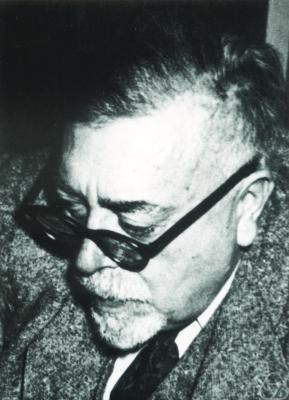
\includegraphics[height=0.42\textheight]{ch11_wiener.jpg}\\[1mm]
\imgcap{Norbert Wiener}
\imgcredit{https://commons.wikimedia.org/wiki/File:Norbert_wiener.jpg}{Foto: Konrad Jacobs, MFO; CC BY-SA 2.0 de; Wikimedia Commons}
\end{column}
\begin{column}{0.66\textwidth}
\begin{itemize}
    \item 1930: analiza armonică generalizată a lui Wiener; 1934: Hincin; autocovarianța și spectrul formează o pereche Fourier
    \item 1942: reprezentarea lui Cramér a unui proces staționar ca suprapunere aleatoare de sinusoide
    \item 1961--1966: ferestre de decalaje \refPar; forma spectrală tipică a variabilelor economice \refGra
    \item 1982: estimarea multitaper \refTho; cauzalitatea în domeniul frecvenței \refGew
    \item 1984--1989: wavelets \refGM, \refDau, \refMal; 1998: ghidul practic \refTC
\end{itemize}
\end{column}
\end{columns}
\end{frame}

\begin{frame}{Cunoscut din TSA și elemente noi}
\itemsize{\small}
\begin{itemize}
    \item Cunoscut (\atschlink{https://danpele.github.io/Time-Series-Analysis/RO/Cursuri/capitol12_analiza_spectrala.pdf}{TSA, Capitolul 12}): frecvențele Fourier, spectrul modelelor ARMA, periodograma și legea ei $\chi^2_2$, netezirea Daniell, ponderarea datelor (taper), testul lui Fisher, o primă privire asupra coerenței și a wavelets
    \item Nou: instrumentele de cercetare
    \begin{itemize}
        \item teoria asimptotică a estimatorilor spectrali: deplasare, varianță, lățime de bandă optimă, benzi de încredere valide, multitaper
        \item inferență asupra co-mișcării: praguri pentru coerență, erorile fazei, corelația dinamică, cauzalitatea pe frecvențe
        \item filtre judecate după cîștig; analiză timp--frecvență cu teste de semnificație care controlează descoperirile false
    \end{itemize}
    \item Studii de caz: Thomson (1982), Croux--Forni--Reichlin (2001), Breitung--Candelon (2006), Baxter--King (1999), Cogley--Nason (1995), Hamilton (2018), Torrence--Compo (1998), Grinsted et al.\ (2004), cu specificațiile din lucrări, pe datele noastre
\end{itemize}
\end{frame}


%=============================================================================
\section{Reprezentarea spectrală}
%=============================================================================

\begin{frame}{Autocovarianța și distribuția spectrală}
\itemsize{\small}
\begin{itemize}
    \item \textbf{Herglotz}: $\gamma(\cdot)$ este autocovarianța unui proces staționar dacă și numai dacă $\gamma(h) = \int_{(-\pi, \pi]} e^{i\omega h}\,dF(\omega)$, cu $F$ nedescrescătoare, continuă la dreapta, mărginită \refBD
    \begin{itemize}
        \item $F$ este \textbf{distribuția spectrală}; dacă $\sum_h|\gamma(h)| < \infty$, $dF(\omega) = f(\omega)\,d\omega$, cu $f(\omega) = \frac{1}{2\pi}\sum_h\gamma(h)e^{-i\omega h}$
    \end{itemize}
    \item $\gamma(0) = \int_{-\pi}^{\pi}f(\omega)\,d\omega$: spectrul este o \textbf{descompunere a varianței pe frecvențe}
    \begin{itemize}
        \item frecvența $\omega$ în radiani pe perioadă; perioada $2\pi/\omega$; date trimestriale: banda ciclului economic de 6--32 de trimestre este $\omega \in [\pi/16, \pi/3]$
    \end{itemize}
    \item Un salt al lui $F$ în $\pm\omega_0$ este un ciclu determinist (un \textbf{spectru de linii}); memoria lungă este un pol al lui $f$ în $\omega = 0$ (\atschlink{https://danpele.github.io/Advanced-Time-Series/RO/Cursuri/capitol10_memorie_lunga_rough_volatility.pdf}{Capitolul 10})
\end{itemize}
\end{frame}

\begin{frame}{Reprezentarea lui Cramér}
\itemsize{\small}
\begin{columns}[T]
\begin{column}{0.32\textwidth}
\centering
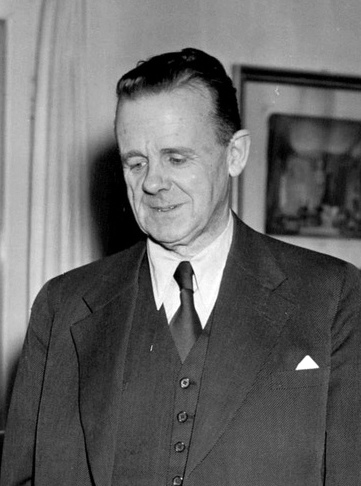
\includegraphics[height=0.4\textheight]{ch11_cramer_1951.jpg}\\[1mm]
\imgcap{Harald Cramér, 1951}
\imgcredit{https://commons.wikimedia.org/wiki/File:Harald_Cram\%C3\%A9r.jpg}{Foto: fotograf necunoscut, Svenska Dagbladet (1951); domeniu public; Wikimedia Commons}
\end{column}
\begin{column}{0.66\textwidth}
\begin{itemize}
    \item Orice proces staționar de medie zero are $X_t = \int_{(-\pi, \pi]} e^{i\omega t}\,dZ(\omega)$ \refBD
    \item $Z$ are \textbf{creșteri ortogonale}: $\E[dZ(\omega)\overline{dZ(\lambda)}] = 0$ pentru $\omega \ne \lambda$, $\E|dZ(\omega)|^2 = dF(\omega)$
    \item Amplitudinile aleatoare de la frecvențe diferite sînt necorelate: componentele de frecvență se pot studia separat
    \item DFT $d(\omega_j) = n^{-1/2}\sum_t x_te^{-i\omega_jt}$ este analogul de eșantion al lui $dZ(\omega_j)$: aproape necorelat între frecvențele Fourier
\end{itemize}
\end{column}
\end{columns}
\end{frame}

\begin{frame}{Filtre liniare în domeniul frecvenței}
\itemsize{\small}
\begin{itemize}
    \item $Y_t = \sum_j a_jX_{t-j}$ cu $\sum_j|a_j| < \infty$: $dZ_Y(\omega) = A(\omega)\,dZ_X(\omega)$, $A(\omega) = \sum_j a_je^{-i\omega j}$ fiind \textbf{funcția de transfer}
    \begin{itemize}
        \item $f_Y(\omega) = |A(\omega)|^2f_X(\omega)$; $|A(\omega)|$ este \textbf{cîștigul}, $\arg A(\omega)$ este \textbf{defazajul}
        \item ponderi simetrice $a_j = a_{-j}$: $A(\omega)$ este real, fără defazaj; proprietatea dorită de orice filtru de tendință și ciclu
    \end{itemize}
    \item Prima diferență: $|1 - e^{-i\omega}|^2 = 2(1 - \cos\omega)$, nulă în $\omega = 0$: diferențierea elimină ciclurile lungi și le amplifică pe cele scurte
    \item Efectul Slutsky: o sumă mobilă a unui zgomot alb are un vîrf în spectru, adică \textbf{cicluri create de filtru}; critica filtrului HP din secțiunea 4 este același fenomen
\end{itemize}
\end{frame}

\begin{frame}{Matricea densităților spectrale}
\itemsize{\small}
\begin{itemize}
    \item Proces vectorial $\mathbf X_t$ (dimensiune $k$): $\mathbf f(\omega) = \frac{1}{2\pi}\sum_h\Gamma(h)e^{-i\omega h}$, $\Gamma(h) = \Cov(\mathbf X_{t+h}, \mathbf X_t)$, o matrice hermitică nenegativă
    \begin{itemize}
        \item VARMA $\Phi(L)\mathbf X_t = \Theta(L)\boldsymbol\varepsilon_t$: $\mathbf f(\omega) = \frac{1}{2\pi}\Phi(e^{-i\omega})^{-1}\Theta(e^{-i\omega})\bSigma\Theta(e^{-i\omega})^*\Phi(e^{-i\omega})^{-*}$
    \end{itemize}
    \item În afara diagonalei: \textbf{spectrul încrucișat} $f_{xy}(\omega) = c_{xy}(\omega) - iq_{xy}(\omega)$ (cospectrul $c$, spectrul în cuadratură $q$)
    \begin{itemize}
        \item $c_{xy}$ este par în $\omega$ (co-mișcare simultană), $q_{xy}$ impar (decalaj); $\int c_{xy} = \Cov(X_t, Y_t)$
    \end{itemize}
    \item Secțiunea 2 estimează diagonala, secțiunea 3 elementele din afara diagonalei, iar secțiunea 4 factorizează $\mathbf f$ pentru a măsura cauzalitatea
\end{itemize}
\end{frame}

\begin{frame}{Varianța pe benzi de frecvență}
\itemsize{\footnotesize}
\begin{center}
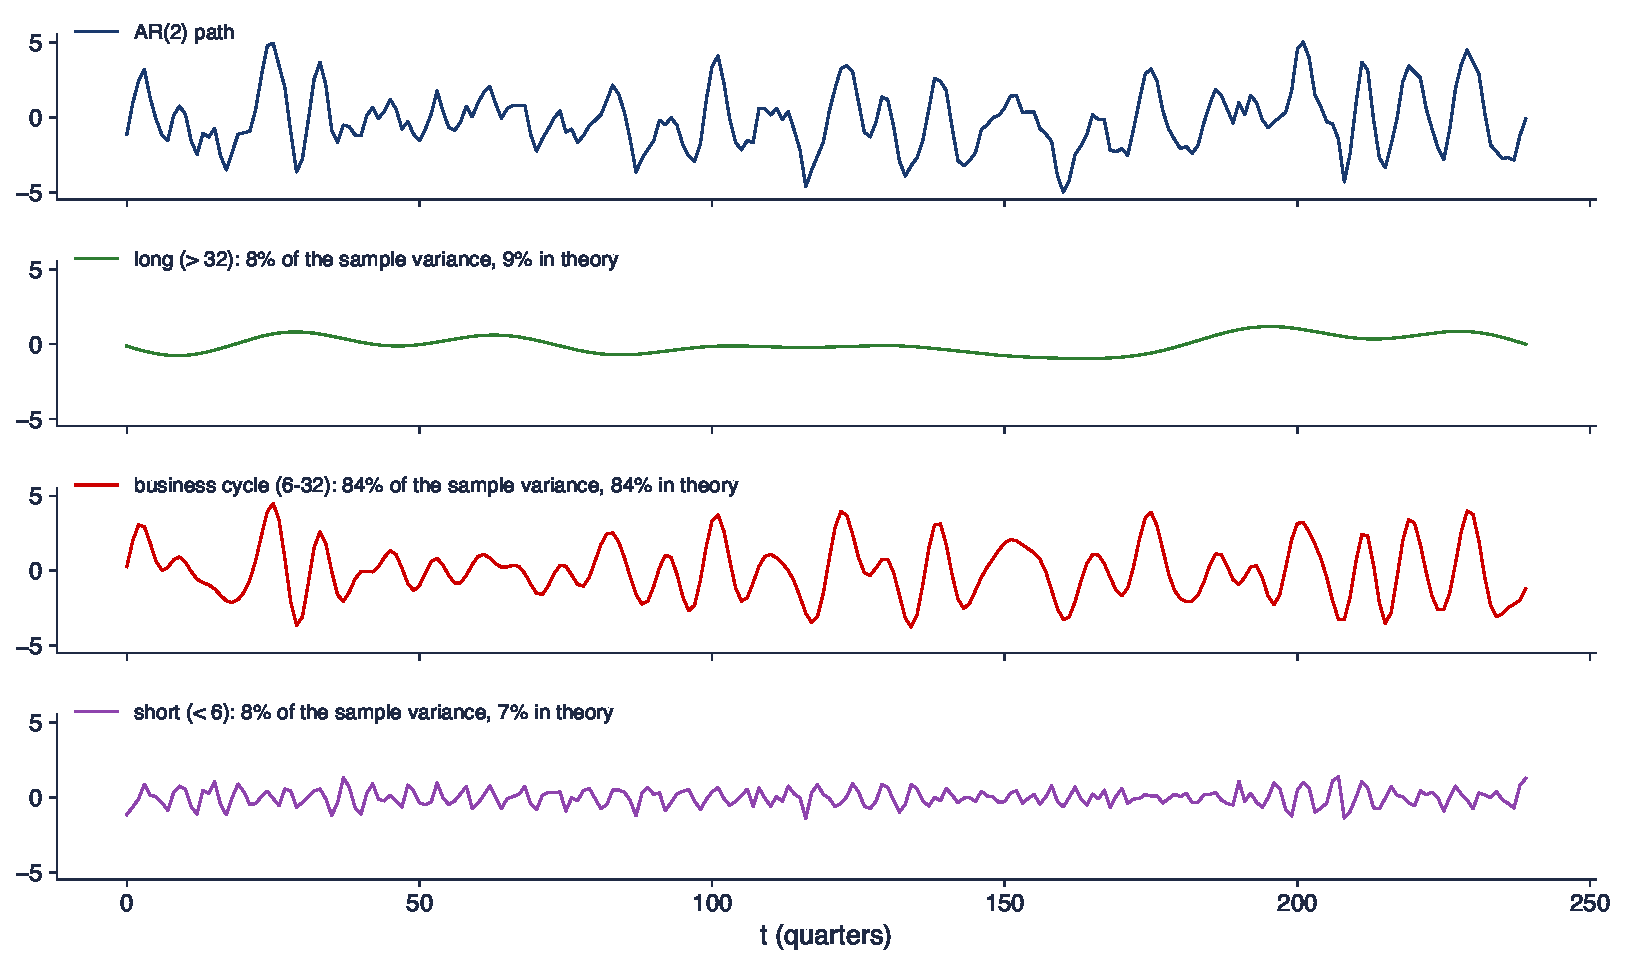
\includegraphics[width=0.97\textwidth,height=0.52\textheight,keepaspectratio]{ats_ch11_bands.pdf}
\end{center}
\vspace{-0.25cm}
\begin{itemize}
    \item O traiectorie AR(2), $X_t = 1{,}3X_{t-1} - 0{,}7X_{t-2} + \varepsilon_t$, 240 de „trimestre”, separată prin DFT în trei benzi; ponderile varianței în eșantion și $2\int_{\mathrm{banda}}f/\gamma(0)$ în teorie
\end{itemize}
\quantlet{ATS\_ch11\_spectral\_estimation}{\qlurl{ATS_ch11_spectral_estimation}}
\end{frame}

\begin{frame}{Interpretarea descompunerii pe benzi}
\itemsize{\small}
\begin{itemize}
    \item Vîrful spectral se află la perioada 9{,}5: 84\% din varianță se află în banda de 6--32 de perioade (în eșantion: 84\%)
    \item Ciclurile lungi și cele scurte au 9\% și 7\% în teorie: cele trei componente sînt necorelate conform teoremei lui Cramér, deci ponderile se adună
    \item „Ciclul economic” al unui AR(2) este un pseudo-ciclu stochastic: amplitudine și lungime neregulate, fără linie în spectru
    \item Filtrele trece-bandă (secțiunea 4) estimează exact această componentă din mijloc pe un eșantion finit
\end{itemize}
\end{frame}

\begin{frame}{Recapitulare: reprezentarea spectrală}
\itemsize{\small}
\begin{itemize}
    \item Spectrul descompune varianța pe frecvențe; Cramér: amplitudini aleatoare necorelate la fiecare frecvență
    \item Un filtru liniar înmulțește spectrul cu pătratul cîștigului; filtrele simetrice nu defazează
    \item Matricea spectrală conține spectrele încrucișate: co-mișcarea și decalajele pe frecvențe
\end{itemize}
\end{frame}


%=============================================================================
\section{Teoria estimării spectrale}
%=============================================================================

\begin{frame}{Limitele periodogramei}
\itemsize{\small}
\begin{itemize}
    \item Pentru un proces liniar $X_t = \sum_j\psi_j\varepsilon_{t-j}$ cu $\sum_j|j|^{1/2}|\psi_j| < \infty$ și $f > 0$: $I(\omega_j) \Rightarrow f(\omega_j)\,\chi^2_2/2$, asimptotic independente pe frecvențe Fourier fixate \refBD
    \begin{itemize}
        \item $\E I(\omega_j) \to f(\omega_j)$, dar $\Var I(\omega_j) \to f(\omega_j)^2$: \textbf{inconsistentă}, varianța nu scade cu $n$
    \end{itemize}
    \item $\E I(\omega) = \int F_n(\omega - \lambda)f(\lambda)\,d\lambda$, $F_n$ fiind nucleul Fejér: lobii laterali scad doar ca $1/(n\omega^2)$, deci puterea se \textbf{scurge} (leakage) de la frecvențele puternice spre cele slabe
    \item Două remedii: \textbf{medierea} frecvențelor vecine (consistență) și \textbf{ponderarea} datelor cu un taper (deplasare); estimatorul multitaper le face pe amîndouă
\end{itemize}
\end{frame}

\begin{frame}{Estimatori cu fereastră de decalaje}
\itemsize{\small}
\begin{itemize}
    \item $\hat f(\omega) = \frac{1}{2\pi}\sum_{|h| < n}k(h/M)\hat\gamma(h)e^{-i\omega h}$, $k$ fiind \textbf{fereastra de decalaje}, $M$ parametrul de trunchiere (lățimea de bandă) \refPar
    \begin{itemize}
        \item echivalent, $\hat f(\omega) = \int W_M(\omega - \lambda)I(\lambda)\,d\lambda$: o medie ponderată a periodogramei cu \textbf{fereastra spectrală} $W_M(\omega) = \frac{1}{2\pi}\sum_h k(h/M)e^{-i\omega h}$
    \end{itemize}
    \item Bartlett $k(u) = 1 - |u|$; Parzen; Tukey--Hanning; pătratic spectral (QS): aceleași nuclee ca estimatorii HAC din \atschlink{https://danpele.github.io/Advanced-Time-Series/RO/Cursuri/capitol0_recapitulare_inferenta.pdf}{Capitolul 0} în $\omega = 0$
    \begin{itemize}
        \item un $W_M$ nenegativ garantează $\hat f \ge 0$ (Bartlett, Parzen, QS); Tukey--Hanning poate deveni negativ
    \end{itemize}
    \item Exponentul caracteristic $q$ și $k_q = \lim_{u \to 0}(1 - k(u))/|u|^q$: Bartlett $q = 1$, $k_1 = 1$; Parzen $q = 2$, $k_2 = 6$; QS $q = 2$, $k_2 = 1{,}42$
\end{itemize}
\end{frame}

\begin{frame}{Ferestre de decalaje și ferestre spectrale}
\itemsize{\footnotesize}
\begin{center}
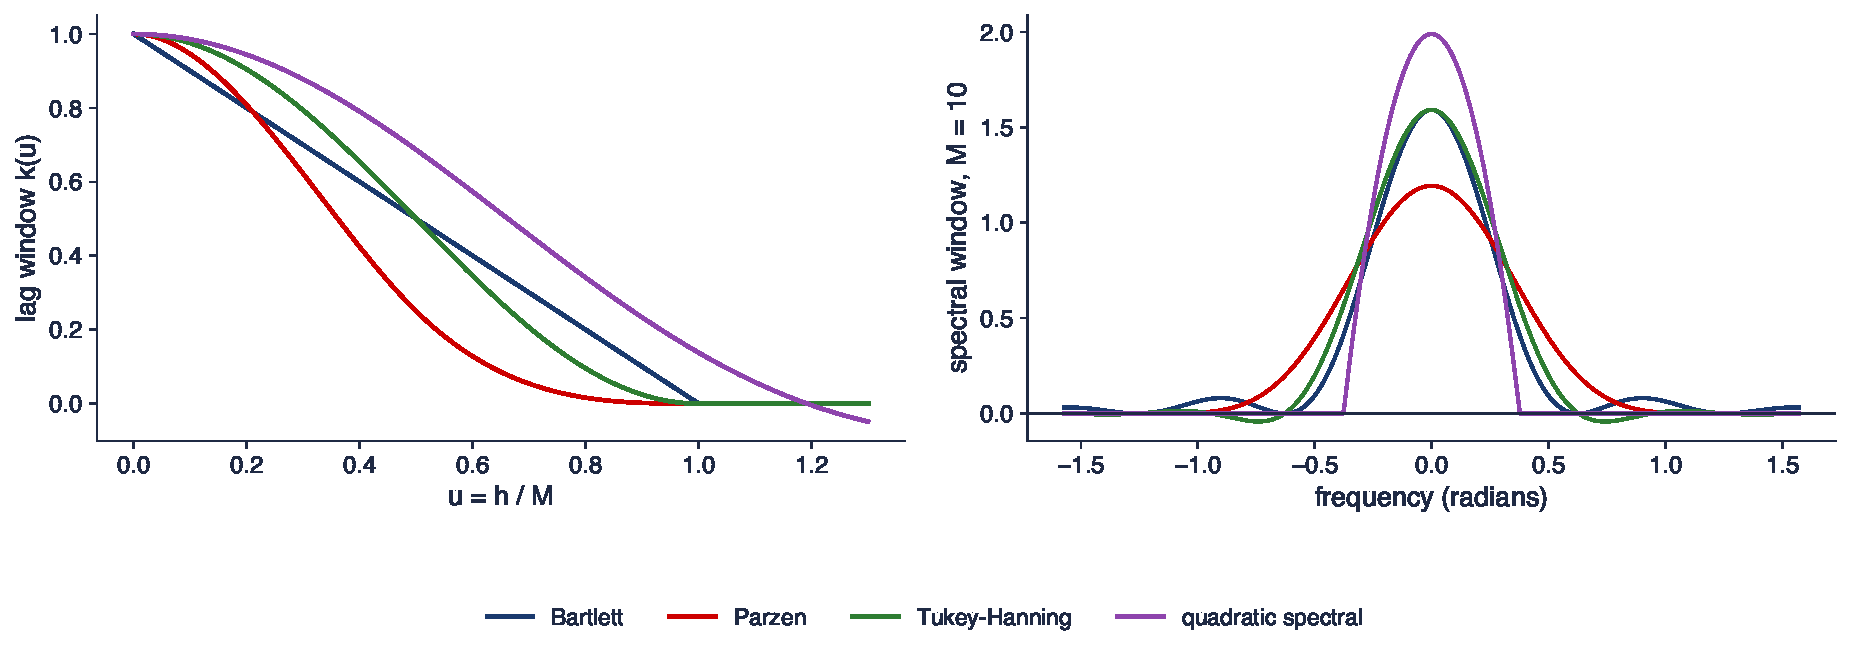
\includegraphics[width=0.97\textwidth,height=0.5\textheight,keepaspectratio]{ats_ch11_kernels.pdf}
\end{center}
\vspace{-0.25cm}
\begin{itemize}
    \item Stînga: $k(u)$; dreapta: fereastra spectrală $W_M(\omega)$ pentru $M = 10$, ponderile pe care fiecare estimator le dă periodogramei în jurul lui $\omega$
\end{itemize}
\quantlet{ATS\_ch11\_spectral\_estimation}{\qlurl{ATS_ch11_spectral_estimation}}
\end{frame}

\begin{frame}{Interpretarea ferestrelor}
\itemsize{\small}
\begin{itemize}
    \item O fereastră $W_M$ îngustă înseamnă deplasare mică și varianță mare; Parzen este cea mai largă la $M = 10$ ($\int k^2 = 0{,}54$ este cel mai mic), QS cea mai îngustă
    \item Bartlett are lobi laterali (scurgere prin fereastra însăși); Tukey--Hanning are ponderi negative
    \item Compararea nucleelor la același $M$ este înșelătoare: comparați-le la aceeași varianță (același număr echivalent de grade de libertate)
    \item Nucleul QS este optim în MSE printre nucleele cu estimări nenegative \refAnd
\end{itemize}
\end{frame}

\begin{frame}{Deplasare, varianță și lățimea de bandă optimă}
\itemsize{\small}
\begin{itemize}
    \item Dacă $M \to \infty$ și $M/n \to 0$: $\hat f(\omega) \to_p f(\omega)$ (\textbf{consistență}) \refPar
    \begin{itemize}
        \item $\Var\hat f(\omega) \approx \frac{M}{n}f(\omega)^2\int k^2(u)\,du$ (dublu în $\omega = 0, \pm\pi$)
        \item $\E\hat f(\omega) - f(\omega) \approx -k_qM^{-q}f^{(q)}(\omega)$, $f^{(q)}(\omega) = \frac{1}{2\pi}\sum_h|h|^q\gamma(h)e^{-i\omega h}$: deplasarea este mare unde spectrul este curbat (vîrfuri)
    \end{itemize}
    \item Minimizînd MSE: $M^* = \big(qk_q^2f^{(q)}(\omega)^2n\,/\,(f(\omega)^2\int k^2)\big)^{1/(2q+1)} \propto n^{1/(2q+1)}$; MSE $\propto n^{-2q/(2q+1)}$
    \begin{itemize}
        \item nucleele cu $q = 2$ converg mai repede ($n^{-4/5}$) decît Bartlett ($n^{-2/3}$)
    \end{itemize}
    \item Inferență: $\nu\hat f(\omega)/f(\omega) \approx \chi^2_\nu$, cu $\nu = 2n/(M\int k^2)$ grade de libertate echivalente; banda este constantă pe scară logaritmică
\end{itemize}
\end{frame}

\begin{frame}{Compromisul deplasare--varianță într-un vîrf spectral}
\itemsize{\footnotesize}
\begin{center}
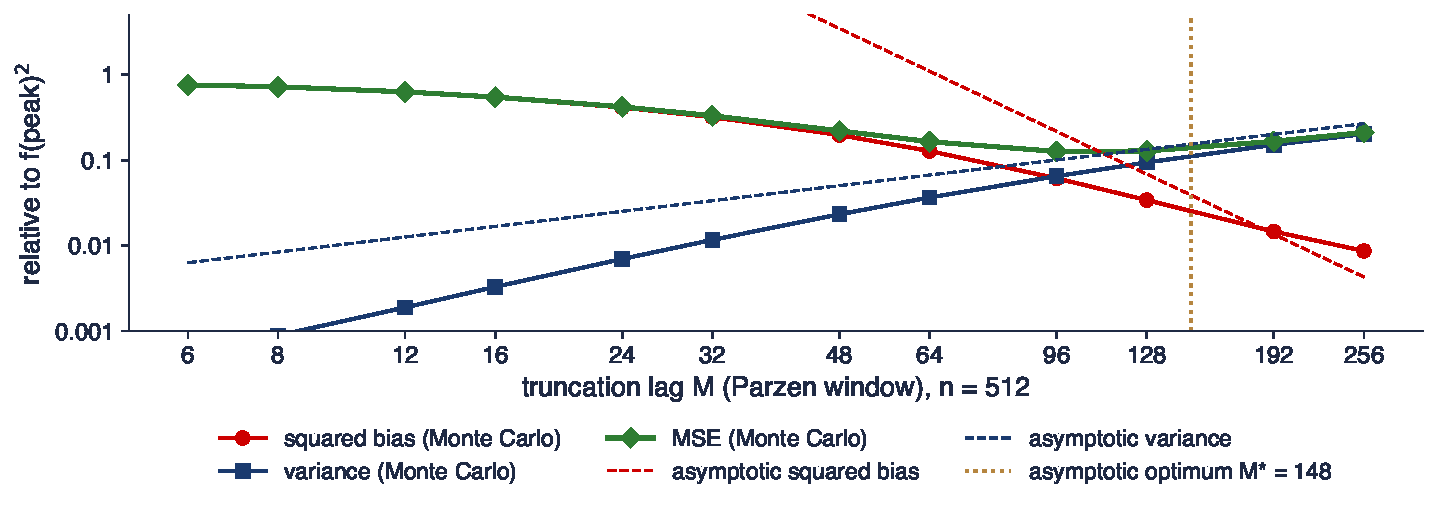
\includegraphics[width=0.97\textwidth,height=0.5\textheight,keepaspectratio]{ats_ch11_bias_variance.pdf}
\end{center}
\vspace{-0.25cm}
\begin{itemize}
    \item Estimatorul Parzen în vîrful (perioada 11{,}1) lui $X_t = 1{,}6X_{t-1} - 0{,}9X_{t-2} + \varepsilon_t$, $n = 512$, 400 de simulări; curbele sînt împărțite la $f(\text{vîrf})^2$; linii întrerupte: formulele asimptotice
\end{itemize}
\quantlet{ATS\_ch11\_spectral\_estimation}{\qlurl{ATS_ch11_spectral_estimation}}
\end{frame}

\begin{frame}{Interpretarea compromisului}
\itemsize{\small}
\begin{itemize}
    \item Cu $M = 12$, RMSE relativ este 0{,}79, aproape în întregime deplasare (0{,}79): o netezire puternică aplatizează vîrful
    \item Optimul Monte Carlo este $M = 96$ (RMSE relativ 0{,}36); formula asimptotică dă $M^* = 148$: același ordin de mărime, dar formula ignoră termenii de deplasare de ordin superior
    \item Varianța asimptotică este precisă doar cînd fereastra este mai îngustă decît vîrful; deplasarea asimptotică explodează pentru $M$ mic
    \item Un vîrf spectral ascuțit cere un $M$ mult mai mare decît ar sugera regula HAC pentru $\omega = 0$: lățimea de bandă este locală
\end{itemize}
\end{frame}

\begin{frame}{Alegerea lățimii de bandă}
\itemsize{\small}
\begin{itemize}
    \item \textbf{Plug-in} \refAnd: aproximăm $f^{(q)}/f$ printr-un model parametric (AR(1)), apoi folosim $M^*$; pentru $\omega = 0$: $M = 1{,}1447(\hat\alpha(1)n)^{1/3}$ (Bartlett), $1{,}3221(\hat\alpha(2)n)^{1/5}$ (QS)
    \begin{itemize}
        \item bun pentru varianțele pe termen lung (\atschlink{https://danpele.github.io/Advanced-Time-Series/RO/Cursuri/capitol0_recapitulare_inferenta.pdf}{Capitolul 0}); slab lîngă vîrfuri ascuțite, unde aproximarea AR(1) este greșită
    \end{itemize}
    \item \textbf{Validare încrucișată} \refHur: minimizăm un criteriu Whittle fără observația $j$, $\sum_j\big[\log\hat f_{-j}(\omega_j) + I(\omega_j)/\hat f_{-j}(\omega_j)\big]$, în $M$
    \item \textbf{Rezoluția}: două vîrfuri mai apropiate decît lățimea de bandă (circa $1/M$ cicluri) se contopesc; stabiliți rezoluția necesară înainte de a privi datele
    \item Raportați estimarea pentru două sau trei lățimi de bandă: concluziile care depind de $M$ nu sînt concluzii
\end{itemize}
\end{frame}

\begin{frame}{Estimarea multitaper}
\itemsize{\small}
\begin{itemize}
    \item \textbf{Taper-ele Slepian (DPSS)} $v^{(k)}$, $k = 0, \dots, K - 1$: șiruri ortonormate de lungime $n$ care maximizează ponderea $\lambda_k$ a energiei lor în $[-W, W]$ \refTho
    \begin{itemize}
        \item aproximativ $2NW$ dintre ele au $\lambda_k \approx 1$; de obicei $K = 2NW - 1$ (de exemplu $NW = 4$, $K = 7$); $W$ este semilățimea de bandă în cicluri
    \end{itemize}
    \item Spectrele proprii $\hat S_k(\omega) = \frac{1}{2\pi}\big|\sum_tv_t^{(k)}x_te^{-i\omega t}\big|^2$; $\hat f^{\mathrm{mt}} = \frac1K\sum_k\hat S_k$
    \begin{itemize}
        \item $\hat S_k$ sînt aproape necorelate: $2K\hat f^{\mathrm{mt}}/f \approx \chi^2_{2K}$; varianță $f^2/K$, deplasare controlată de concentrarea taper-elor
    \end{itemize}
    \item \textbf{Ponderi adaptive}: $d_k(\omega) = \sqrt{\lambda_k}f(\omega)/(\lambda_kf(\omega) + (1 - \lambda_k)\sigma^2)$, iterate; reduc ponderea taper-elor cu scurgeri acolo unde $f$ este mic \refPWa
    \item Alternative cu aceeași logică: taper-ele sinus \refRS; medierea Welch a segmentelor ponderate \refWel
\end{itemize}
\end{frame}

\begin{frame}{Taper-ele Slepian}
\itemsize{\footnotesize}
\begin{center}
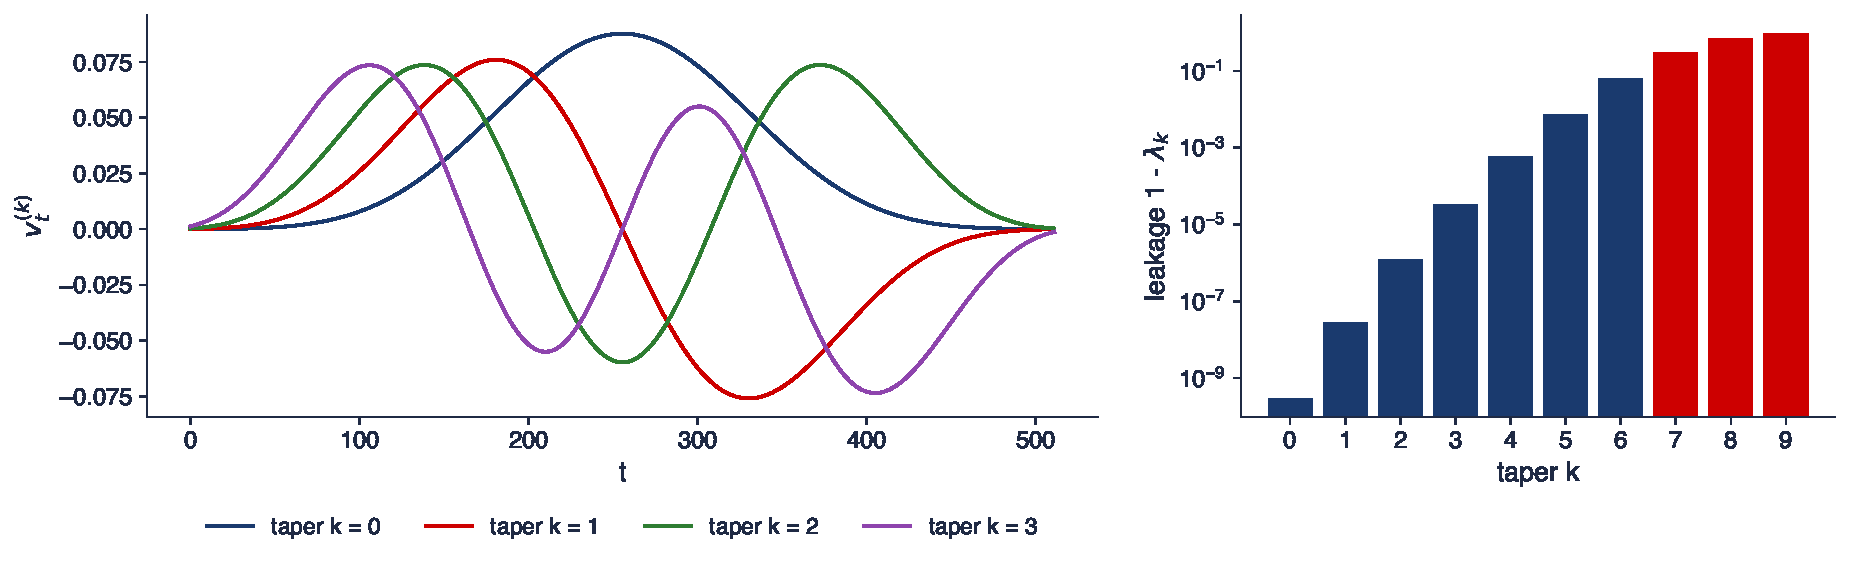
\includegraphics[width=0.97\textwidth,height=0.48\textheight,keepaspectratio]{ats_ch11_dpss.pdf}
\end{center}
\vspace{-0.25cm}
\begin{itemize}
    \item $n = 512$, $NW = 4$: primele patru taper-e și scurgerea $1 - \lambda_k$ a primelor zece (albastru: $k < 2NW - 1$)
\end{itemize}
\quantlet{ATS\_ch11\_spectral\_estimation}{\qlurl{ATS_ch11_spectral_estimation}}
\end{frame}

\begin{frame}{Interpretarea taper-elor}
\itemsize{\small}
\begin{itemize}
    \item Taper-ul $k$ are $k$ treceri prin zero: taper-ele de ordin mare ponderează capetele eșantionului, deci împreună folosesc toate datele
    \item Scurgerea crește repede cu $k$: $\lambda_6 = 0{,}937$, dar $\lambda_7 = 0{,}70$ și $\lambda_8 = 0{,}30$; dincolo de $2NW - 1$ taper-ele nu mai sînt utile
    \item Un singur taper Hann aruncă extremitățile; estimarea multitaper recuperează această informație ca grade de libertate suplimentare
    \item $NW$ este singura alegere de calibrare: fixează împreună rezoluția $2W = 2NW/n$ și varianța $f^2/K$
\end{itemize}
\end{frame}

\begin{frame}{Scurgerea spectrală pe un spectru cu domeniu dinamic mare}
\itemsize{\footnotesize}
\begin{center}
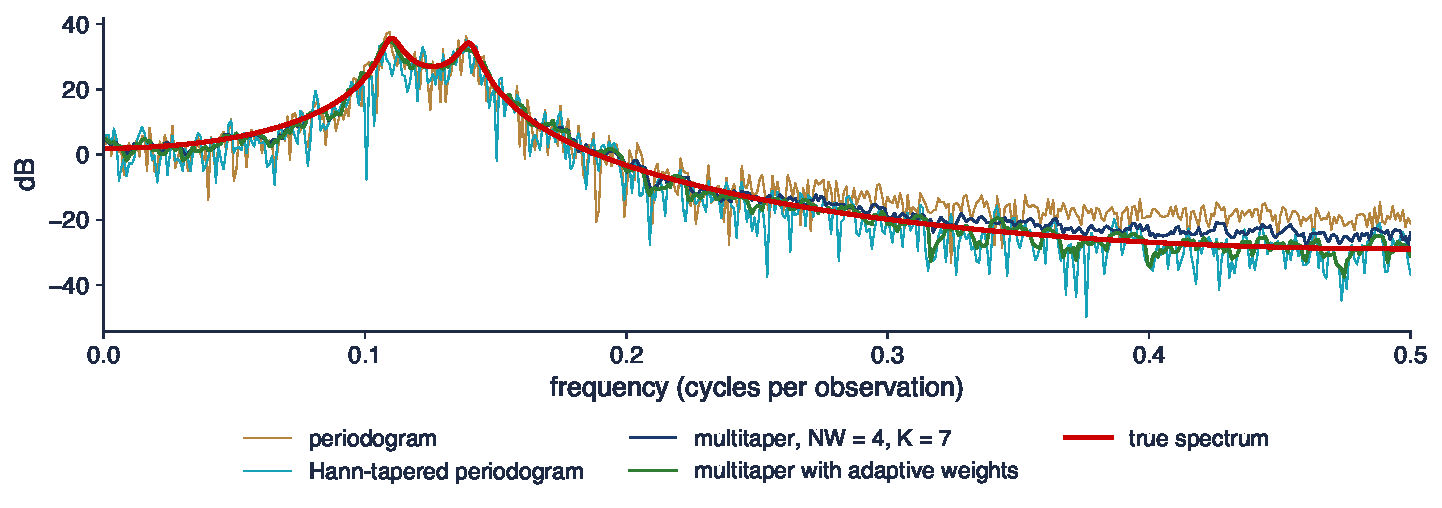
\includegraphics[width=0.97\textwidth,height=0.5\textheight,keepaspectratio]{ats_ch11_leakage.pdf}
\end{center}
\vspace{-0.25cm}
\begin{itemize}
    \item Modelul AR(4) al lui Percival și Walden (1993), $n = 1024$, 65 dB între vîrf și minim; o traiectorie simulată (cu scurgerea mediană din 21)
\end{itemize}
\quantlet{ATS\_ch11\_spectral\_estimation}{\qlurl{ATS_ch11_spectral_estimation}}
\end{frame}

\begin{frame}{Interpretarea scurgerii}
\itemsize{\small}
\begin{itemize}
    \item Deplasarea medie la frecvențe peste 0,3 cicluri (200 de simulări): periodograma +11{,}2 dB, taper Hann \ensuremath{-}2{,}5 dB, multitaper +6{,}3 dB, multitaper adaptiv \ensuremath{-}0{,}8 dB
    \item Periodograma brută umple minimul cu putere scursă din vîrfuri: o mediere suplimentară nu ar ajuta, deplasarea este în fiecare ordonată
    \item Cu ponderi egale, taper-ele de ordin mare, care au scurgeri, contaminează încă minimul; ponderile adaptive o elimină
    \item Datele economice au rareori domenii de 60 dB, dar spectrele nivelurilor, cu un vîrf în zero ca la o rădăcină unitară, le au: aplicați un taper sau o prealbire înainte de estimare
\end{itemize}
\end{frame}

\begin{frame}{Cinci estimatori într-un experiment Monte Carlo}
\itemsize{\footnotesize}
\begin{center}
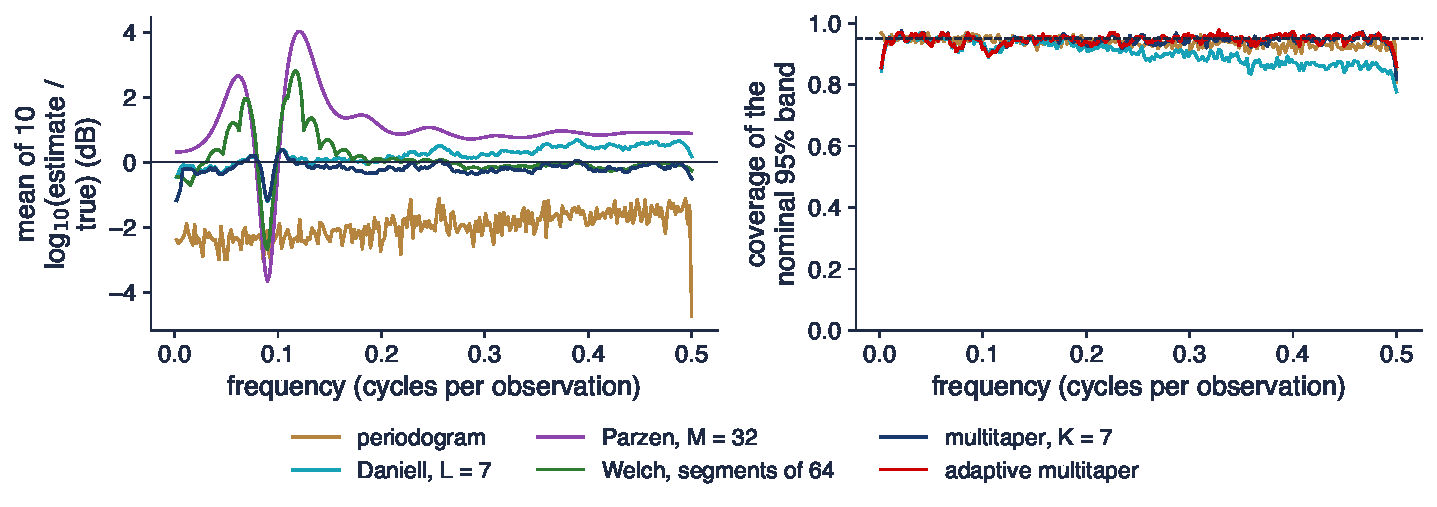
\includegraphics[width=0.97\textwidth,height=0.5\textheight,keepaspectratio]{ats_ch11_mt_mc.pdf}
\end{center}
\vspace{-0.25cm}
\begin{itemize}
    \item $X_t = 1{,}6X_{t-1} - 0{,}9X_{t-2} + \varepsilon_t$, $n = 512$, 400 de simulări: deplasarea medie în logaritmi pe frecvențe și acoperirea benzilor $\chi^2$ nominale de 95\%
\end{itemize}
\quantlet{ATS\_ch11\_spectral\_estimation}{\qlurl{ATS_ch11_spectral_estimation}}
\end{frame}

\begin{frame}{Interpretarea experimentului Monte Carlo}
\itemsize{\small}
\begin{itemize}
    \item Abaterea standard a lui $10\log_{10}(\hat f/f)$: periodograma 5{,}6 dB, Daniell 1{,}8, multitaper 1{,}7, Parzen 0{,}9, Welch 1{,}1
    \item În vîrf: Parzen \ensuremath{-}2{,}3 dB, Welch \ensuremath{-}1{,}4 dB, multitaper \ensuremath{-}0{,}5 dB; valoarea \ensuremath{-}2{,}0 dB a periodogramei este media lui $\log\chi^2_2/2$, nu o deplasare în niveluri
    \item Acoperirea benzii de 95\%: multitaper 94{,}3\%, adaptiv 94{,}6\%, Daniell 90{,}3\% (banda lui ignoră deplasarea de pe pante)
    \item Multitaper este singurul estimator de aici care are simultan deplasare mică, varianță mică și benzi corecte
\end{itemize}
\end{frame}

\begin{frame}{Producția industrială: România și zona euro}
\itemsize{\footnotesize}
\begin{center}
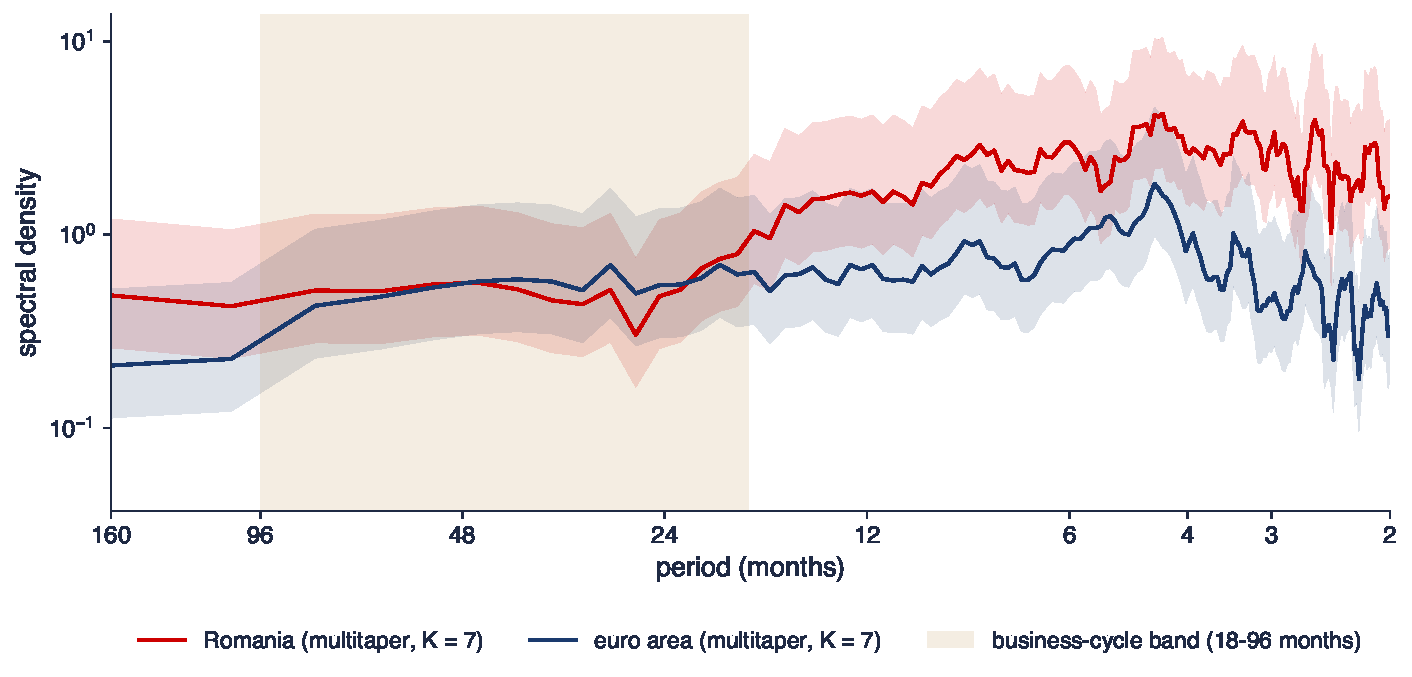
\includegraphics[width=0.97\textwidth,height=0.5\textheight,keepaspectratio]{ats_ch11_ip_spectrum.pdf}
\end{center}
\vspace{-0.25cm}
\begin{itemize}
    \item Creșterea lunară a producției industriale (ajustată sezonier și pentru zilele lucrătoare), februarie 2000 -- iulie 2026, 318 luni; multitaper $NW = 4$ cu benzi de 95\%
\end{itemize}
\quantlet{ATS\_ch11\_ip\_spectrum}{\qlurl{ATS_ch11_ip_spectrum}}
\end{frame}

\begin{frame}{Interpretarea spectrelor producției industriale}
\itemsize{\small}
\begin{itemize}
    \item Creșterea lunară este dominată de perioadele scurte: ciclurile sub 6 luni au 77\% din varianță în România și 69\% în zona euro
    \item Banda ciclului economic (18--96 de luni) are 2{,}1\% (România) și 7{,}3\% (zona euro): ratele de creștere ascund ciclurile vizibile în niveluri (cîștigul primei diferențe)
    \item România este mai volatilă (abaterea standard 3{,}61 față de 1{,}98), iar surplusul este la frecvențe înalte, unde benzile nu se suprapun: zgomot, revizuiri și efecte de calendar reziduale
    \item La perioade de peste 12 luni, cele două spectre nu se pot distinge în interiorul benzilor
\end{itemize}
\end{frame}

\begin{frame}{Linii în spectru: testul F al lui Thomson}
\itemsize{\small}
\begin{itemize}
    \item Modelul: $x_t = \mu\cos(\omega_0t + \phi) + $ zgomot cu spectru neted; sub o linie, fiecare DFT ponderat este $Y_k(\omega_0) \approx \mu U_k(0)$, $U_k(0) = \sum_tv^{(k)}_t$ \refTho
    \begin{itemize}
        \item $\hat\mu(\omega) = \sum_kU_k(0)Y_k(\omega)/\sum_kU_k(0)^2$; $F(\omega) = (K - 1)|\hat\mu|^2\sum_kU_k(0)^2/\sum_k|Y_k - \hat\mu U_k(0)|^2 \sim F_{2, 2K - 2}$
    \end{itemize}
    \item O regresie a coeficienților proprii pe mediile taper-elor, frecvență cu frecvență: separă o linie deterministă de un vîrf stochastic, ceea ce testul lui Fisher (TSA) nu poate
    \item Aplicație: sezonalitatea reziduală este o mulțime de linii la $k/12$ cicluri pe lună; efectele zilelor lucrătoare sînt linii la 0,348 și 0,432 cicluri pe lună
    \item Testarea la sute de frecvențe: așteptați circa 1\% respingeri false la nivelul de 1\%; testați doar frecvențe stabilite dinainte
\end{itemize}
\end{frame}

\begin{frame}{Sezonalitatea reziduală în producția industrială a României}
\itemsize{\footnotesize}
\begin{center}
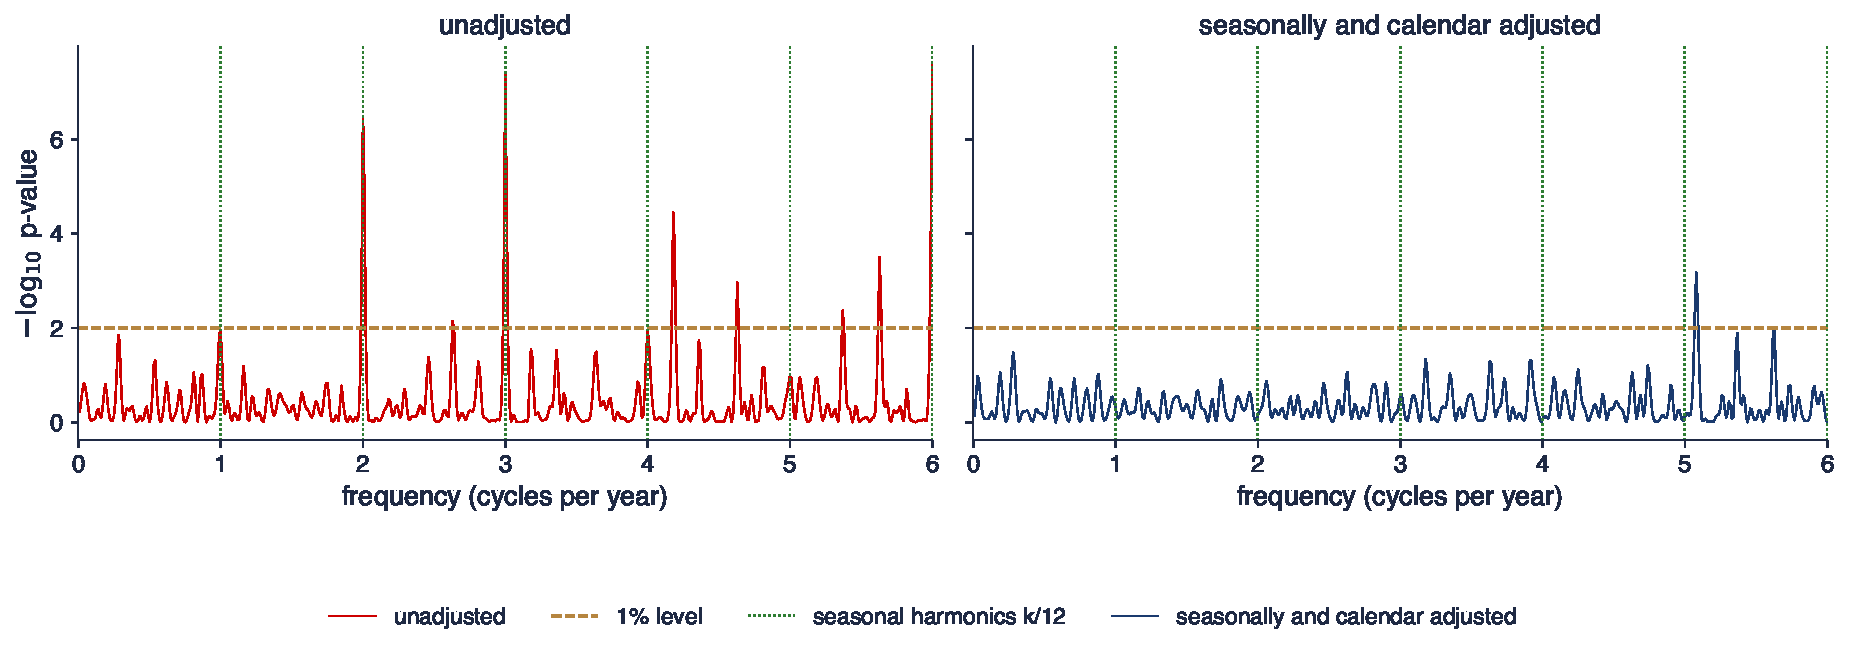
\includegraphics[width=0.97\textwidth,height=0.5\textheight,keepaspectratio]{ats_ch11_ftest.pdf}
\end{center}
\vspace{-0.25cm}
\begin{itemize}
    \item Testul F armonic ($NW = 4$, $K = 7$) pe creșterea lunară, seria neajustată și seria ajustată; liniile punctate: cele șase frecvențe sezoniere
\end{itemize}
\quantlet{ATS\_ch11\_ip\_spectrum}{\qlurl{ATS_ch11_ip_spectrum}}
\end{frame}

\begin{frame}{Interpretarea testului F}
\itemsize{\small}
\begin{itemize}
    \item Seria neajustată: 3 din 6 armonici sezoniere sînt linii la 1\% ($p$ $<$ 0{,}0001 și $<$ 0{,}0001 la 2 și 3 cicluri pe an); armonica anuală este la limită ($p$ = 0{,}012)
    \item O linie puternică la 4,18 cicluri pe an ($p$ $<$ 0{,}0001): frecvența zilelor lucrătoare, un efect de calendar, nu sezonalitate
    \item Seria ajustată: niciuna dintre cele șase armonici nu este semnificativă și nu există nicio linie la frecvența zilelor lucrătoare ($p$ = 0{,}22): ajustarea trece această verificare
    \item Armonica anuală este slabă deoarece sezonalitatea românească nu este o sinusoidă pură: puterea ei se află în armonicile superioare
\end{itemize}
\end{frame}

\begin{frame}{Recapitulare: teoria estimării spectrale}
\itemsize{\small}
\begin{itemize}
    \item Periodograma este asimptotic nedeplasată, dar inconsistentă și cu scurgeri; netezirea aduce consistență, iar taper-ul aduce deplasare mică
    \item Lățimea de bandă este o alegere deplasare--varianță cu $M^* \propto n^{1/(2q+1)}$; vîrfurile cer ferestre înguste
    \item Multitaper: benzi $\chi^2_{2K}$ care își respectă nivelul, ponderi adaptive împotriva scurgerii și un test F pentru linii
\end{itemize}
\end{frame}


%=============================================================================
\section{Două serii: coerență, fază și cauzalitate}
%=============================================================================

\begin{frame}{Coerența, faza și cîștigul}
\itemsize{\small}
\begin{itemize}
    \item \textbf{Coerența pătratică} $\kappa^2_{xy}(\omega) = |f_{xy}(\omega)|^2/(f_x(\omega)f_y(\omega)) \in [0, 1]$: $R^2$ al regresiei lui $dZ_y(\omega)$ pe $dZ_x(\omega)$
    \begin{itemize}
        \item invariantă la filtrarea fiecărei serii cu un filtru inversabil: coerența nu depinde de felul în care sînt transformate seriile
    \end{itemize}
    \item \textbf{Faza} $\phi_{xy}(\omega) = \arg f_{xy}(\omega)$, cu $\gamma_{xy}(h) = \Cov(x_{t+h}, y_t)$: dacă $y_t = x_{t-d}$, atunci $f_{xy} = e^{i\omega d}f_x$, faza $\omega d > 0$: $x$ conduce cu $\phi/\omega$ perioade
    \begin{itemize}
        \item faza este definită modulo $2\pi$: un avans de $d$ și o întîrziere de $2\pi/\omega - d$ dau aceeași fază; interpretați-o doar unde coerența este semnificativă
    \end{itemize}
    \item \textbf{Cîștigul} $|f_{xy}(\omega)|/f_x(\omega)$: coeficientul de regresie al lui $y$ pe $x$ la frecvența $\omega$
\end{itemize}
\end{frame}

\begin{frame}{Inferență pentru coerență și fază}
\itemsize{\small}
\begin{itemize}
    \item Periodograma încrucișată brută dă $\hat\kappa^2 \equiv 1$ la orice frecvență: coerența \textbf{trebuie} netezită (aici: mediată pe $K$ taper-e)
    \begin{itemize}
        \item sub $\kappa^2 = 0$, cu $L$ ordonate independente mediate: $\Pr(\hat\kappa^2 > c) = (1 - c)^{L-1}$, deci pragul de 5\% este $1 - 0{,}05^{1/(L-1)}$
    \end{itemize}
    \item $\hat\kappa^2$ este deplasat în sus cînd $\kappa^2$ este mic; intervale de încredere prin transformarea Fisher $\tanh^{-1}\hat\kappa$ \refSS
    \begin{itemize}
        \item faza: $\mathrm{se}(\hat\phi) \approx \sqrt{(1/\hat\kappa^2 - 1)/(2L)}$; crește foarte mult cînd coerența scade
    \end{itemize}
    \item Deplasarea din nealiniere: un decalaj mare $d$ rotește faza în interiorul benzii de netezire și scade $\hat\kappa^2$; aliniați seriile (sau aplicați o prealbire) mai întîi
\end{itemize}
\end{frame}

\begin{frame}{România și zona euro: coerență, fază și cîștig}
\itemsize{\footnotesize}
\begin{center}
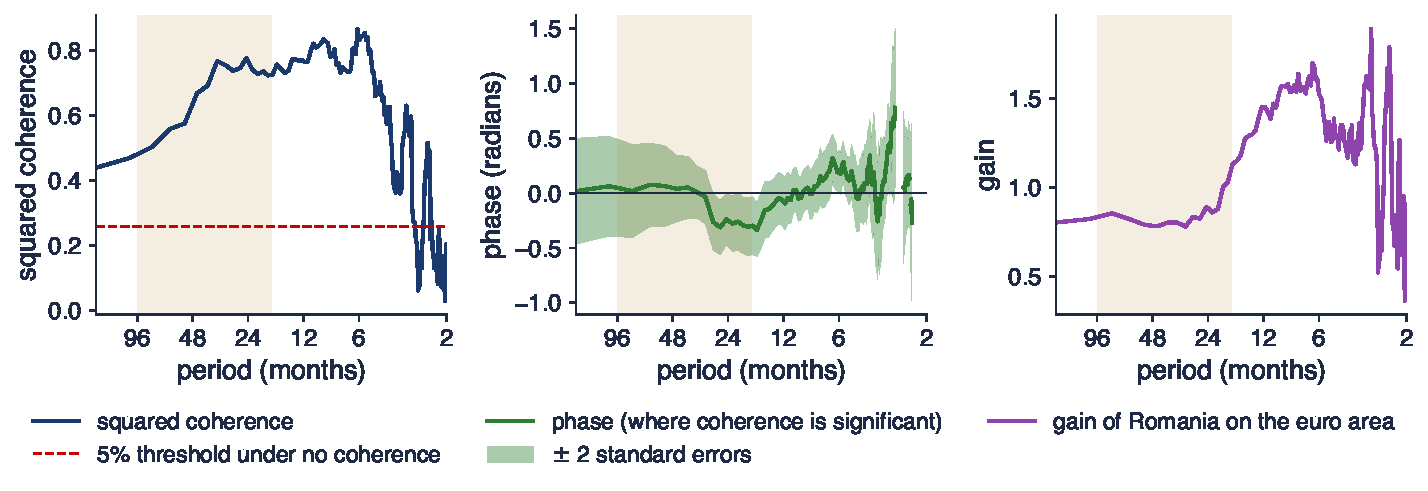
\includegraphics[width=0.97\textwidth,height=0.48\textheight,keepaspectratio]{ats_ch11_coherence.pdf}
\end{center}
\vspace{-0.25cm}
\begin{itemize}
    \item Creșterea lunară a producției industriale, zona euro ($x$) și România ($y$); multitaper $NW = 6$, $K = 11$; zona colorată: 18--96 de luni
\end{itemize}
\quantlet{ATS\_ch11\_cross\_spectrum}{\qlurl{ATS_ch11_cross_spectrum}}
\end{frame}

\begin{frame}{Interpretarea spectrului încrucișat}
\itemsize{\small}
\begin{itemize}
    \item Coerența medie este 0{,}69 în banda ciclului economic și 0{,}47 sub 12 luni; pragul de 5\% este 0{,}26: semnificativă la 100\% din frecvențele ciclului economic și la 71\% din cele scurte
    \item Faza este aproape de zero: avansul median implicat este de 0{,}5 luni, în interiorul a două erori standard: industria românească se mișcă odată cu zona euro în aceeași lună
    \item Cîștigul este 0{,}85 la frecvențele ciclului economic și 1{,}24 la cele scurte: România amplifică șocurile din zona euro doar la frecvențe înalte
    \item Corelația simplă (0{,}66) amestecă aceste benzi; coerența separă zonele cu co-mișcare puternică de cele cu zgomot
\end{itemize}
\end{frame}

\begin{frame}{Corelația dinamică}
\itemsize{\small}
\begin{itemize}
    \item \refCFR: $\rho_{xy}(\omega) = c_{xy}(\omega)/\sqrt{f_x(\omega)f_y(\omega)} \in [-1, 1]$, corelația componentelor reale (în fază) la frecvența $\omega$
    \begin{itemize}
        \item spre deosebire de coerență, are \textbf{semn} și nu este umflată de mișcarea defazată: $\kappa^2 = \rho^2 + (q_{xy}/\sqrt{f_xf_y})^2$
    \end{itemize}
    \item Pe o bandă $\Lambda$: $\rho_{xy}(\Lambda) = \int_\Lambda c_{xy}/\sqrt{\int_\Lambda f_x\int_\Lambda f_y}$; pe $[0, \pi]$ este corelația obișnuită
    \begin{itemize}
        \item este egală cu corelația seriilor filtrate trece-bandă: o cale în domeniul frecvenței pentru ceea ce secțiunea 4 face cu filtre
    \end{itemize}
    \item \textbf{Coeziunea}: o medie ponderată a corelațiilor $\rho_{xy}(\omega)$ pe perechi într-un grup de țări; CFR o folosesc pentru ciclurile economice din zona euro
\end{itemize}
\end{frame}

\begin{frame}{Cauzalitatea Granger pe frecvențe}
\itemsize{\footnotesize}
\begin{itemize}
    \item \refGew: VAR bivariat, inovații normalizate astfel încît inovația lui $x$ să fie necorelată cu inovația transformată a lui $y$; atunci $f_x(\omega) = \frac{1}{2\pi}\big(|\tilde H_{xx}|^2\tilde\sigma_{xx} + |\tilde H_{xy}|^2\tilde\sigma_{yy}\big)$
    \begin{itemize}
        \item $M_{y \to x}(\omega) = \ln\big(2\pi f_x(\omega)/(|\tilde H_{xx}(\omega)|^2\tilde\sigma_{xx})\big) \ge 0$: partea din $f_x(\omega)$ care provine de la $y$
        \item $\frac{1}{\pi}\int_0^\pi M_{y \to x}(\omega)\,d\omega = \ln(\sigma^2_{x|x}/\sigma^2_{x|x,y})$, măsura Granger din domeniul timpului (sub o condiție slabă)
    \end{itemize}
    \item \refBC: $M_{y \to x}(\omega) = 0$ dacă și numai dacă $\sum_{j=1}^p\psi_j\cos(j\omega) = 0$ și $\sum_{j=1}^p\psi_j\sin(j\omega) = 0$, $\psi_j$ fiind coeficienții lui $y_{t-j}$ în ecuația lui $x$
    \begin{itemize}
        \item două restricții liniare: un test $F(2, T - 2p - 1)$ la fiecare $\omega$; cu $p \le 2$ ele fixează toți $\psi_j$, deci testul este același la orice frecvență
    \end{itemize}
    \item BC arată că testul se extinde la VAR cointegrate (cauzalitate pe termen lung în $\omega = 0$); testele punctuale pe frecvențe nu sînt un test comun
\end{itemize}
\end{frame}

\begin{frame}{Cauzează zona euro industria românească și la ce frecvențe?}
\itemsize{\footnotesize}
\begin{center}
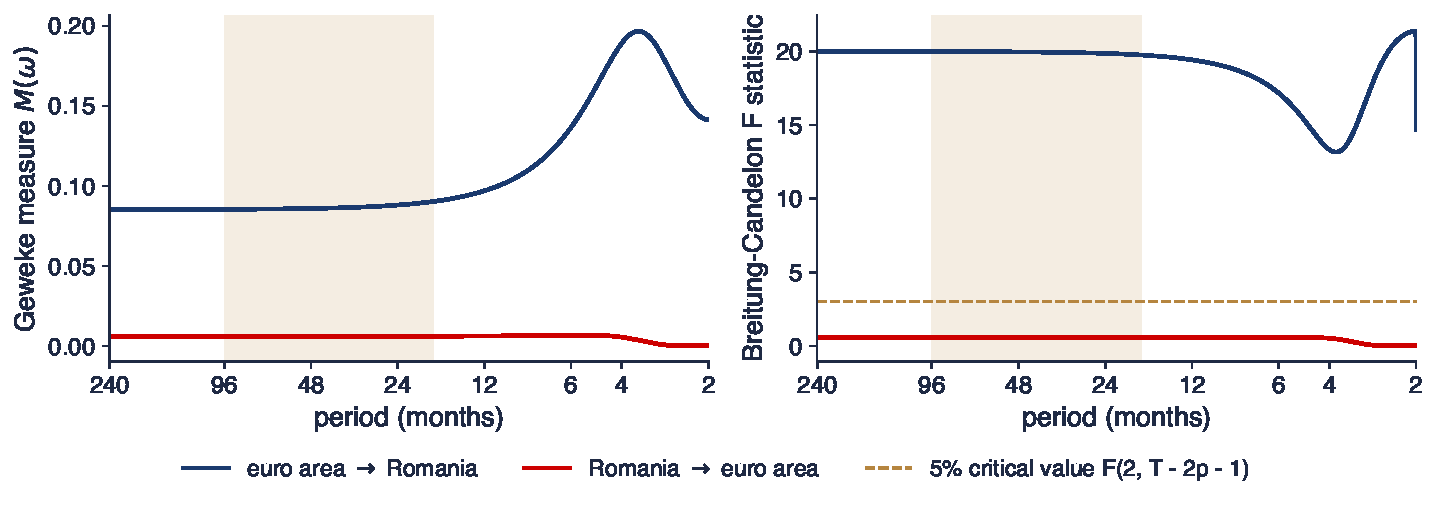
\includegraphics[width=0.97\textwidth,height=0.48\textheight,keepaspectratio]{ats_ch11_causality.pdf}
\end{center}
\vspace{-0.25cm}
\begin{itemize}
    \item VAR(3) pentru creșterea lunară a producției industriale (ordinul ales prin AIC, cel puțin 3); stînga: măsurile Geweke; dreapta: statistica $F$ Breitung--Candelon cu valoarea critică de 5\% 3{,}03
\end{itemize}
\quantlet{ATS\_ch11\_causality}{\qlurl{ATS_ch11_causality}}
\end{frame}

\begin{frame}{Interpretarea cauzalității în domeniul frecvenței}
\itemsize{\small}
\begin{itemize}
    \item Zona euro $\to$ România: măsura Geweke totală 0{,}146 (integrala curbei: 0{,}145); România $\to$ zona euro: 0{,}004
    \item Măsura este 0{,}087 în banda ciclului economic și 0{,}168 la perioade sub 6 luni: creșterea trecută din zona euro prezice creșterea românească mai ales la orizonturi scurte
    \item Testul BC respinge la 100\% din frecvențe pentru zona euro $\to$ România și la nicio frecvență în cealaltă direcție
    \item O economie mică și deschisă își urmează piața principală, nu invers; profilul pe frecvențe arată ce tip de șoc se transmite cel mai repede
\end{itemize}
\end{frame}

\begin{frame}{Recapitulare: două serii}
\itemsize{\small}
\begin{itemize}
    \item Coerența este un $R^2$ pe frecvențe; trebuie netezită și testată față de $1 - \alpha^{1/(L-1)}$
    \item Faza dă avansurile și întîrzierile, modulo $2\pi$, doar unde coerența este semnificativă; corelația dinamică păstrează semnul
    \item Geweke descompune cauzalitatea Granger pe frecvențe; Breitung--Candelon o testează prin două restricții liniare
\end{itemize}
\end{frame}


%=============================================================================
\section{Filtre și ciclul economic}
%=============================================================================

\begin{frame}{Filtre trece-bandă}
\itemsize{\small}
\begin{itemize}
    \item Filtrul ideal pentru perioadele $[p_l, p_u]$: cîștig 1 pe $[2\pi/p_u, 2\pi/p_l]$, 0 în rest; ponderi $b_0 = (\omega_2 - \omega_1)/\pi$, $b_j = (\sin j\omega_2 - \sin j\omega_1)/(\pi j)$: în număr infinit
    \item \refBK: trunchiem la $K$ și adăugăm o constantă astfel încît $\sum_{j=-K}^Ka_j = 0$: elimină o rădăcină unitară și o tendință liniară; simetric, fără defazaj
    \begin{itemize}
        \item recomandarea trimestrială: BK(6, 32, $K = 12$); prețul: $K$ observații pierdute la fiecare capăt; $a_0 = 0{,}28$
    \end{itemize}
    \item \refCF: minimizăm $\E[(y^{\mathrm{ideal}}_t - \hat y_t)^2 \mid y_1, \dots, y_n]$ presupunînd un mers aleator: ponderi asimetrice, variabile în timp, care folosesc tot eșantionul
    \begin{itemize}
        \item nicio observație pierdută, dar defazaje lîngă capete și dependență de ipoteza mersului aleator
    \end{itemize}
    \item Banda ciclului economic de 6--32 de trimestre (1,5--8 ani) urmează definiția Burns și Mitchell, preluată de \refBK
\end{itemize}
\end{frame}

\begin{frame}{Filtrul Hodrick--Prescott}
\itemsize{\small}
\begin{columns}[T]
\begin{column}{0.3\textwidth}
\centering
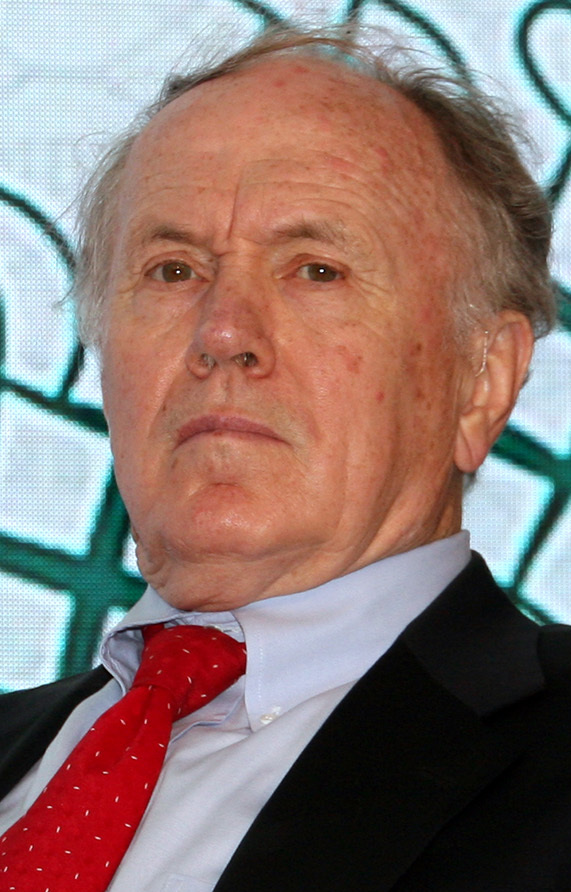
\includegraphics[height=0.4\textheight]{ch11_prescott_2015.jpg}\\[1mm]
\imgcap{Edward C.\ Prescott, 2015}
\imgcredit{https://commons.wikimedia.org/wiki/File:Edward_C_Prescott_2015_(cropped).jpg}{Foto: Narodowy Bank Polski (2015); CC BY-SA 2.0; Wikimedia Commons}
\end{column}
\begin{column}{0.68\textwidth}
\begin{itemize}
    \item $\hat\tau = \arg\min_\tau\sum_t(y_t - \tau_t)^2 + \lambda\sum_t(\Delta^2\tau_t)^2 = (I + \lambda D'D)^{-1}y$ \refHP
    \item Cîștigul ciclului pe un eșantion infinit: $G(\omega) = \dfrac{4\lambda(1 - \cos\omega)^2}{1 + 4\lambda(1 - \cos\omega)^2}$, un filtru trece-sus
    \item Este netezitorul Kalman al unei tendințe liniare locale cu raportul semnal--zgomot $1/\lambda$ (TSA și ATS, \atschlink{https://danpele.github.io/Advanced-Time-Series/RO/Cursuri/capitol6_modele_spatiul_starilor_filtrare_bayesiana.pdf}{Capitolul 6})
    \item $\lambda = 1600$ pentru trimestre; scalarea Ravn--Uhlig $\lambda \propto s^4$: 129\,600 pentru luni, 6,25 pentru ani \refRU
\end{itemize}
\end{column}
\end{columns}
\end{frame}

\begin{frame}{Critica lui Hamilton}
\itemsize{\small}
\begin{itemize}
    \item \refHam: „de ce nu ar trebui să folosiți niciodată filtrul HP”
    \begin{itemize}
        \item (1) aplicat unui mers aleator, HP produce un ciclu cu o dinamică creată de filtru \refCN
        \item (2) valorile de la sfîrșitul eșantionului diferă mult de cele pe care același filtru le dă după ce sosesc date noi (unilateral față de bilateral)
        \item (3) $\lambda$ implicat de un model statistic estimat pe date este departe de 1600
    \end{itemize}
    \item Alternativa: \textbf{filtrul de regresie} $y_{t+h} = \beta_0 + \beta_1y_t + \dots + \beta_py_{t-p+1} + v_{t+h}$, ciclul este $\hat v_{t+h}$; trimestrial $h = 8$, $p = 4$
    \begin{itemize}
        \item unilateral prin construcție; consistent pentru eroarea de prognoză a unei clase largi de procese nestaționare; pentru un mers aleator $v_{t+h} = y_{t+h} - y_t$
    \end{itemize}
    \item Răspunsuri: filtrul HP iterat (boosting) \refPS; un filtru Hamilton modificat pentru timp real \refQW; dezbaterea privește ce cîștig doriți
\end{itemize}
\end{frame}

\begin{frame}{Filtre judecate după cîștig}
\itemsize{\footnotesize}
\begin{center}
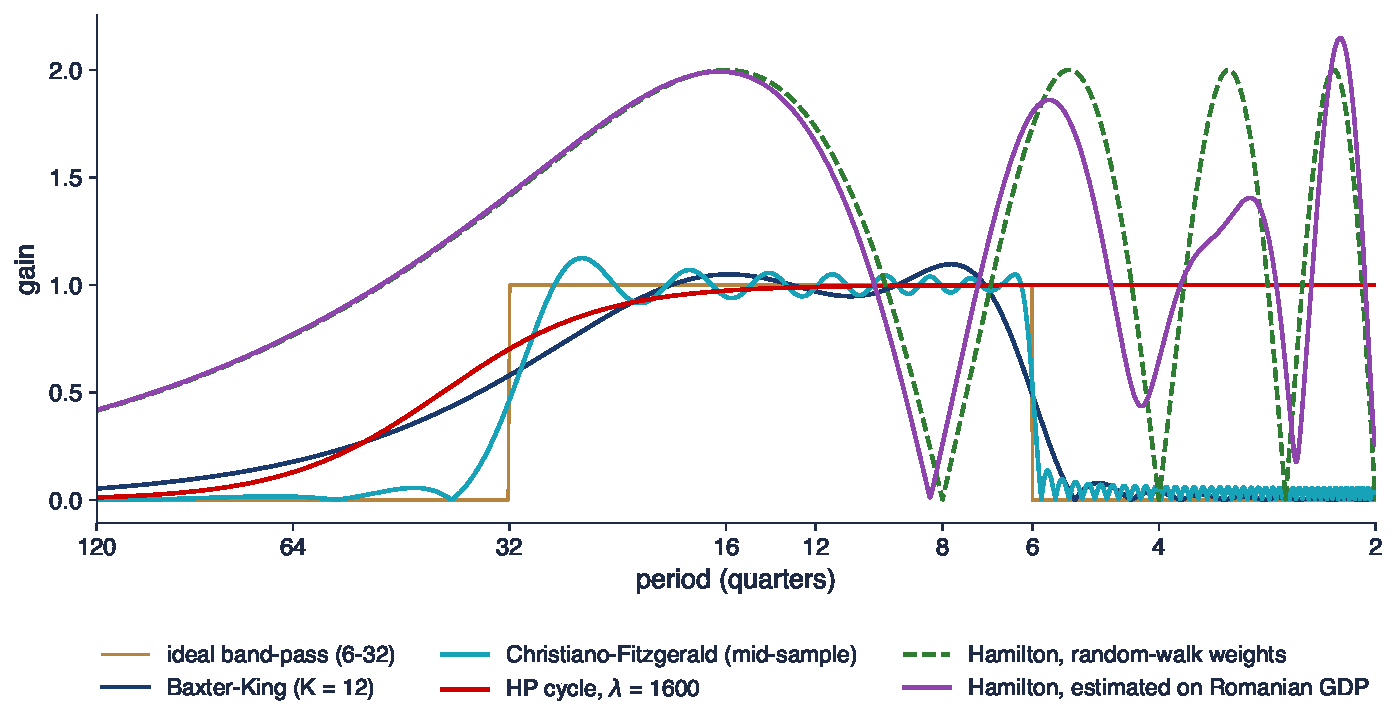
\includegraphics[width=0.97\textwidth,height=0.5\textheight,keepaspectratio]{ats_ch11_gains.pdf}
\end{center}
\vspace{-0.25cm}
\begin{itemize}
    \item Cîștigul de la nivel la ciclu, pe perioade în trimestre; Christiano--Fitzgerald: ponderile din mijlocul unui eșantion de 126 de trimestre; Hamilton: $h = 8$, $p = 4$
\end{itemize}
\quantlet{ATS\_ch11\_filters}{\qlurl{ATS_ch11_filters}}
\end{frame}

\begin{frame}{Interpretarea cîștigurilor}
\itemsize{\small}
\begin{itemize}
    \item HP este un filtru trece-sus: cîștig 0{,}70 la 32 de trimestre, 0{,}49 la 40 și încă 0{,}16 la 60: „ciclul HP” conține cicluri mai lungi de 8 ani
    \item BK oscilează în jurul lui 1 (maximum 1{,}10) și lasă să treacă 0{,}41 din ciclul de 40 de trimestre; CF este mai aproape de forma ideală în mijlocul eșantionului
    \item Filtrul lui Hamilton nu este trece-bandă: cîștig 2{,}00 la 16 trimestre și 0{,}00 la 8 (pentru ponderile mersului aleator); ponderile estimate pentru România (suma 0{,}97) dau 1{,}99 și 0{,}26
    \item Fiecare filtru își definește propriul ciclu: comparați ciclurile doar după ce ați comparat cîștigurile
\end{itemize}
\end{frame}

\begin{frame}{Un ciclu creat de filtru}
\itemsize{\footnotesize}
\begin{center}
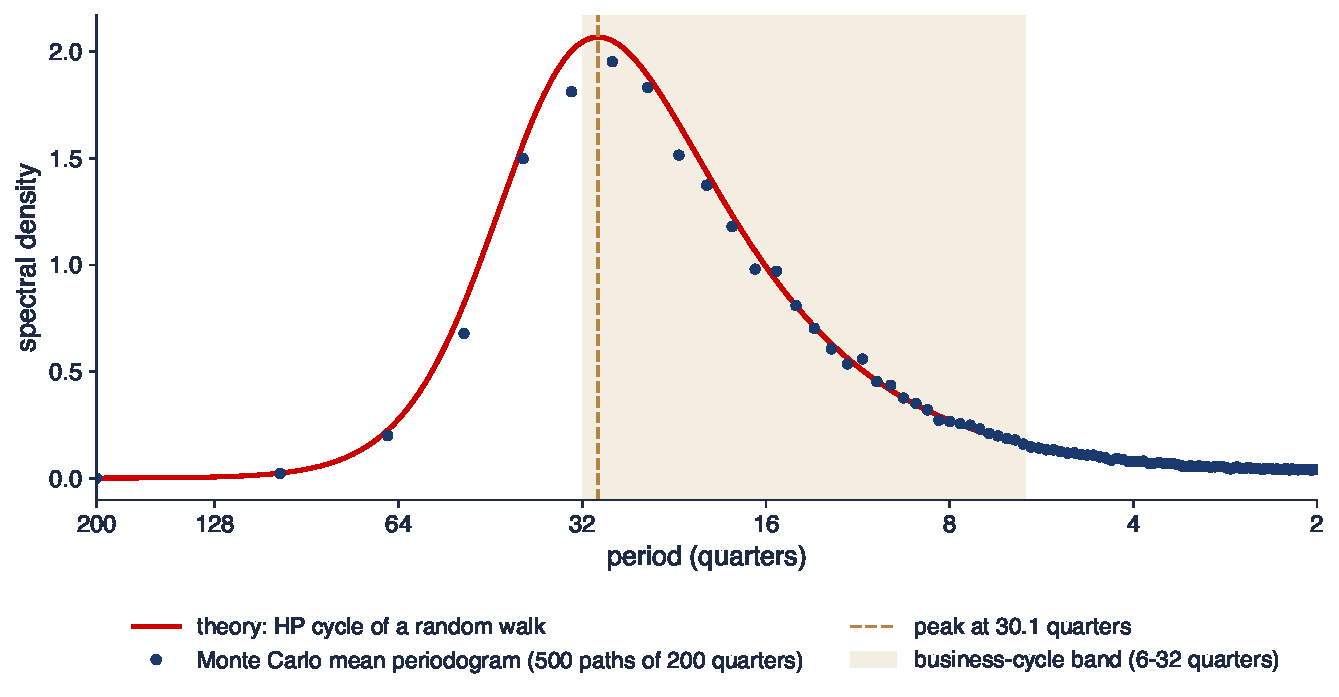
\includegraphics[width=0.97\textwidth,height=0.5\textheight,keepaspectratio]{ats_ch11_cogley_nason.pdf}
\end{center}
\vspace{-0.25cm}
\begin{itemize}
    \item Spectrul ciclului HP ($\lambda = 1600$) al unui mers aleator: $G(\omega)^2/(2\pi\cdot2(1 - \cos\omega))$ și periodograma medie a unor mersuri aleatoare simulate filtrate HP
\end{itemize}
\quantlet{ATS\_ch11\_filters}{\qlurl{ATS_ch11_filters}}
\end{frame}

\begin{frame}{Interpretarea ciclului fals}
\itemsize{\small}
\begin{itemize}
    \item Un mers aleator nu are niciun ciclu, totuși ciclul lui HP are un vîrf la perioada de 30{,}1 trimestre (7{,}5 ani); simulare: 28{,}6
    \item Derivarea (Seminarul 11, A1): maximizăm $u^3/(1 + 4\lambda u^2)^2$ în $u = 1 - \cos\omega$: $u^* = \sqrt{3/(4\lambda)}$; replică \refCN
    \item Vîrful se află în banda ciclului economic: „faptele stilizate” calculate din ciclurile HP pot fi proprietăți ale filtrului
    \item Scalarea Ravn--Uhlig păstrează vîrful în jur de 7,5 ani și la frecvențele lunară și anuală (Seminarul 11, A2)
\end{itemize}
\end{frame}

\begin{frame}{Ciclurile economice ale României după patru filtre}
\itemsize{\footnotesize}
\begin{center}
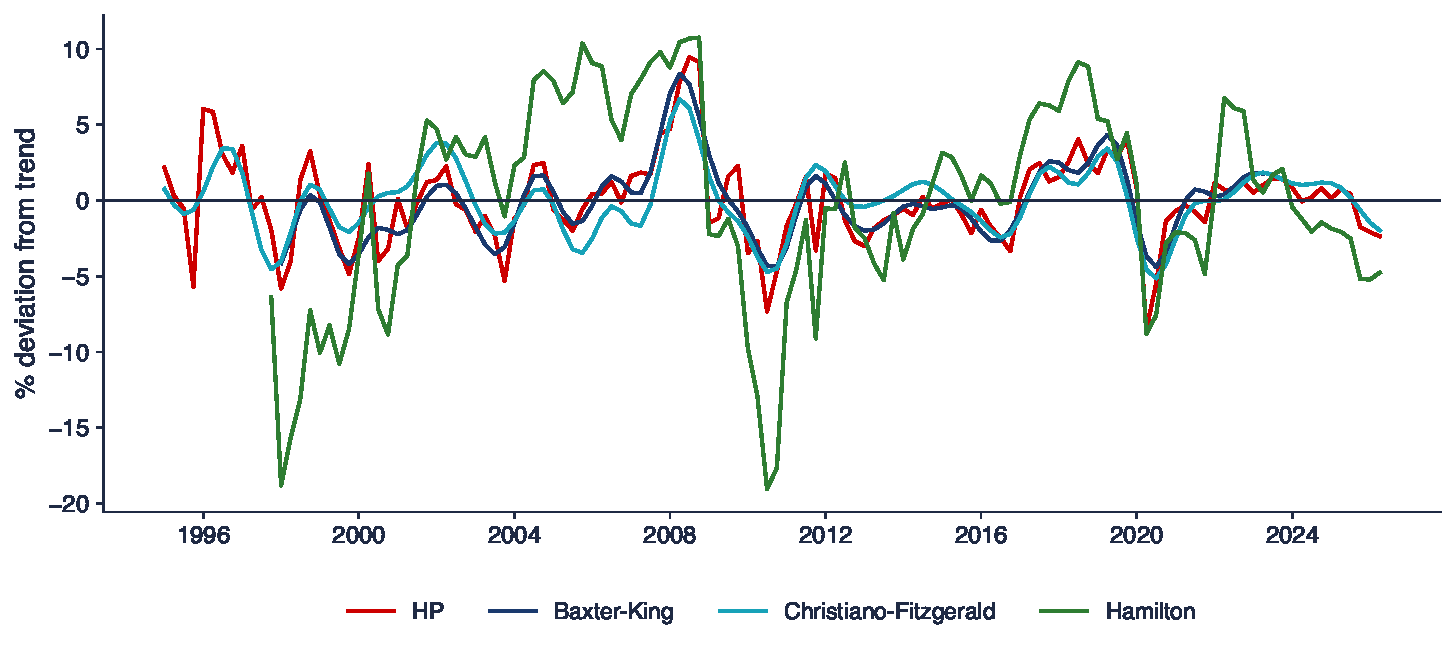
\includegraphics[width=0.97\textwidth,height=0.5\textheight,keepaspectratio]{ats_ch11_ro_cycles.pdf}
\end{center}
\vspace{-0.25cm}
\begin{itemize}
    \item 100 $\times$ logaritmul PIB-ului real al României, T1 1995 -- T2 2026; HP ($\lambda = 1600$), BK(6, 32, 12), CF(6, 32, mers aleator cu derivă), Hamilton ($h = 8$, $p = 4$)
\end{itemize}
\quantlet{ATS\_ch11\_filters}{\qlurl{ATS_ch11_filters}}
\end{frame}

\begin{frame}{Interpretarea ciclurilor României}
\itemsize{\footnotesize}
\begin{itemize}
    \item Toate cele patru filtre situează la fel vîrful din 2008 (HP 9{,}5\%, BK 8{,}4\%) și minimul din T3 2010 (HP \ensuremath{-}7{,}3\%, BK \ensuremath{-}4{,}4\%)
    \item Amplitudinile diferă: abaterea standard HP 2{,}9, BK 2{,}5, CF 2{,}2, Hamilton 6{,}6; ciclul Hamilton este o eroare de prognoză la 8 trimestre, cu un minim de \ensuremath{-}19{,}0\%
    \item Corelații: BK--HP 0{,}84, BK--CF 0{,}84, HP--Hamilton 0{,}69, CF--Hamilton 0{,}49
    \item Poziția de azi este incertă: HP \ensuremath{-}2{,}4\%, CF \ensuremath{-}2{,}0\%, Hamilton \ensuremath{-}4{,}8\% în T2 2026; BK se oprește în T2 2023
\end{itemize}
\end{frame}

\begin{frame}{Problema capetelor de eșantion}
\itemsize{\footnotesize}
\begin{center}
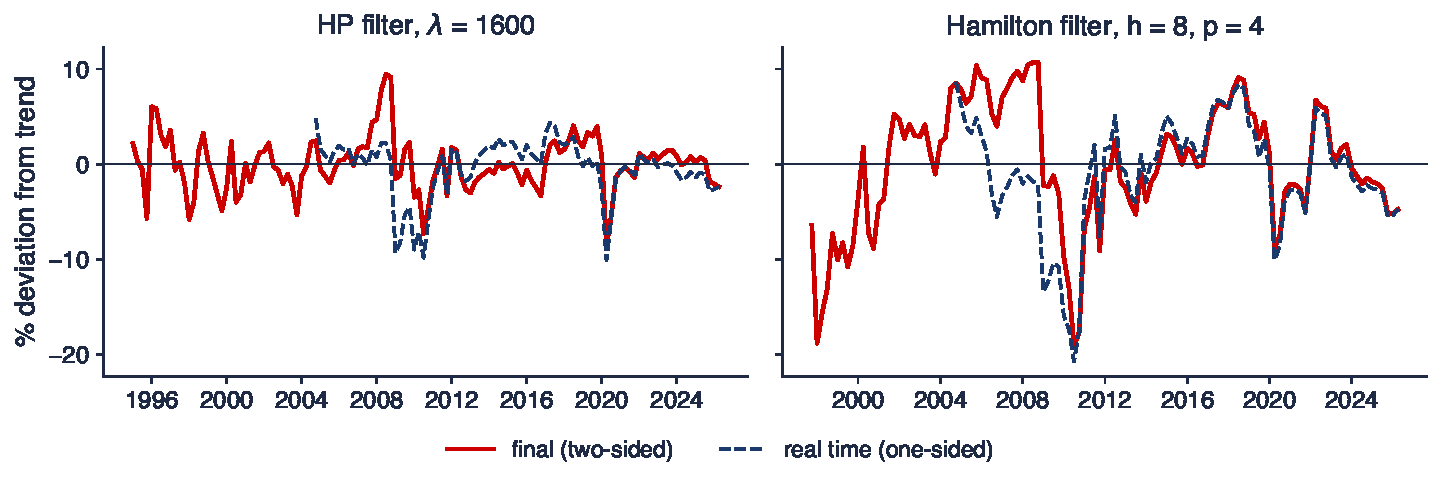
\includegraphics[width=0.97\textwidth,height=0.5\textheight,keepaspectratio]{ats_ch11_endpoint.pdf}
\end{center}
\vspace{-0.25cm}
\begin{itemize}
    \item PIB-ul României: ciclul la fiecare dată calculat cu datele disponibile la acea dată (timp real) și cu tot eșantionul (final), din T4 2004
\end{itemize}
\quantlet{ATS\_ch11\_filters}{\qlurl{ATS_ch11_filters}}
\end{frame}

\begin{frame}{Interpretarea revizuirilor în timp real}
\itemsize{\footnotesize}
\begin{itemize}
    \item HP: revizuirea medie pătratică 2{,}8 puncte, cît ciclul însuși (abaterea standard 2{,}8); corelația dintre ciclul în timp real și cel final 0{,}57; semnul greșit în 38\% din trimestre
    \item Hamilton: corelația 0{,}76, semnul greșit în 24\% din trimestre; dar revizuirea este de 4{,}6 puncte, deoarece regresia se reestimează pe eșantioane scurte într-o economie în tranziție
    \item Filtrul HP în timp real a văzut doar o mică parte din boom-ul din 2008: deviația PIB-ului de care avea nevoie politica economică era tocmai cea pe care o măsura cel mai prost
    \item Raportați proprietățile în timp real ale oricărei estimări a deviației; estimarea finală nu este o informație pe care o avea cineva
\end{itemize}
\end{frame}

\begin{frame}{Măsurarea sincronizării ciclurilor economice}
\itemsize{\small}
\begin{itemize}
    \item Corelația ciclurilor filtrate; depinde de filtru (cîștig) și de cîteva episoade mari
    \item \textbf{Concordanța} \refHPa: $C = \frac1T\sum_t[S_{xt}S_{yt} + (1 - S_{xt})(1 - S_{yt})]$, $S_t = 1$ în expansiune (aici: ciclul peste tendință); comparați cu $p_xp_y + (1 - p_x)(1 - p_y)$ sub independență
    \item Corelația dinamică pe banda ciclului economic \refCFR, care nu cere niciun filtru
    \item Evidența pentru Europa Centrală și de Est: o meta-analiză a 35 de publicații arată că unele țări aveau deja corelații mari cu zona euro și că metoda de estimare schimbă semnificativ corelația \refFK
\end{itemize}
\end{frame}

\begin{frame}{România și zona euro: sincronizarea în timp}
\itemsize{\footnotesize}
\begin{center}
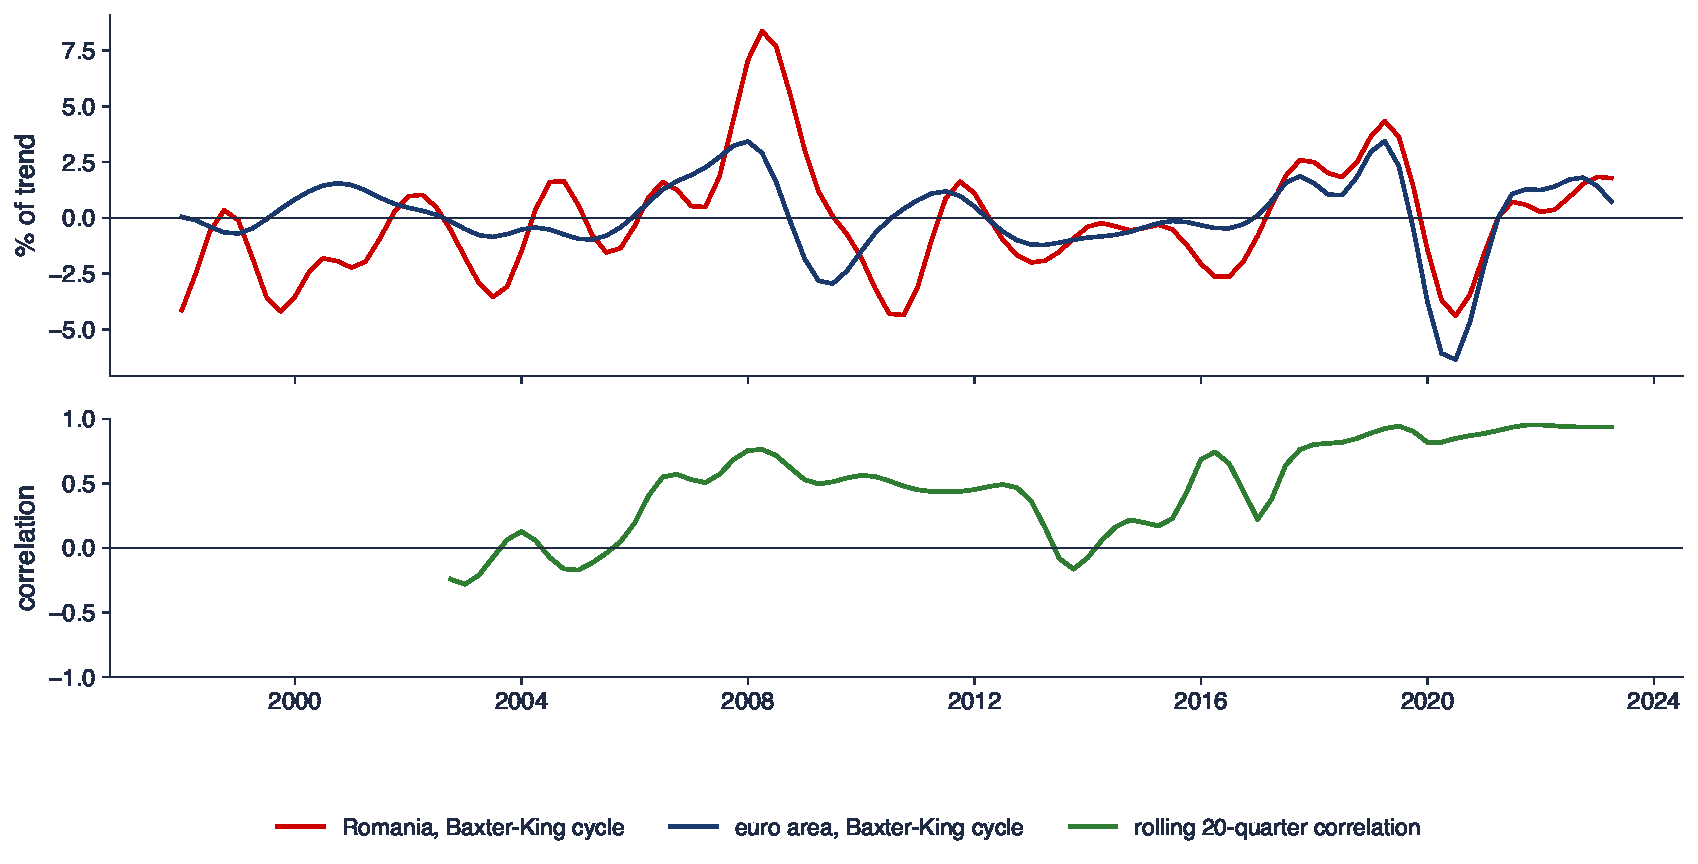
\includegraphics[width=0.97\textwidth,height=0.5\textheight,keepaspectratio]{ats_ch11_sync.pdf}
\end{center}
\vspace{-0.25cm}
\begin{itemize}
    \item Ciclurile Baxter--King ale PIB-ului real, T1 1998 -- T2 2023, și corelația lor mobilă pe 20 de trimestre
\end{itemize}
\quantlet{ATS\_ch11\_filters}{\qlurl{ATS_ch11_filters}}
\end{frame}

\begin{frame}{Interpretarea sincronizării}
\itemsize{\small}
\begin{itemize}
    \item Corelația ciclurilor: 0{,}54 pe tot eșantionul; 0{,}34 înainte de 2008, 0{,}47 în 2008--2012, 0{,}90 în 2013--2019, 0{,}96 din 2020
    \item Concordanța 0{,}75 față de 0{,}50 sub independență: cele două economii sînt împreună peste sau sub tendință în majoritatea timpului
    \item Ciclul României este mai amplu (abaterea standard 2{,}5 față de 1{,}7): sincronizat ca moment, nu ca amplitudine
    \item Corelația de după 2020 este determinată de un singur șoc comun (pandemia): cîteva trimestre pot face un deceniu să pară sincronizat
\end{itemize}
\end{frame}

\begin{frame}{Corelația dinamică cu zona euro}
\itemsize{\footnotesize}
\begin{center}
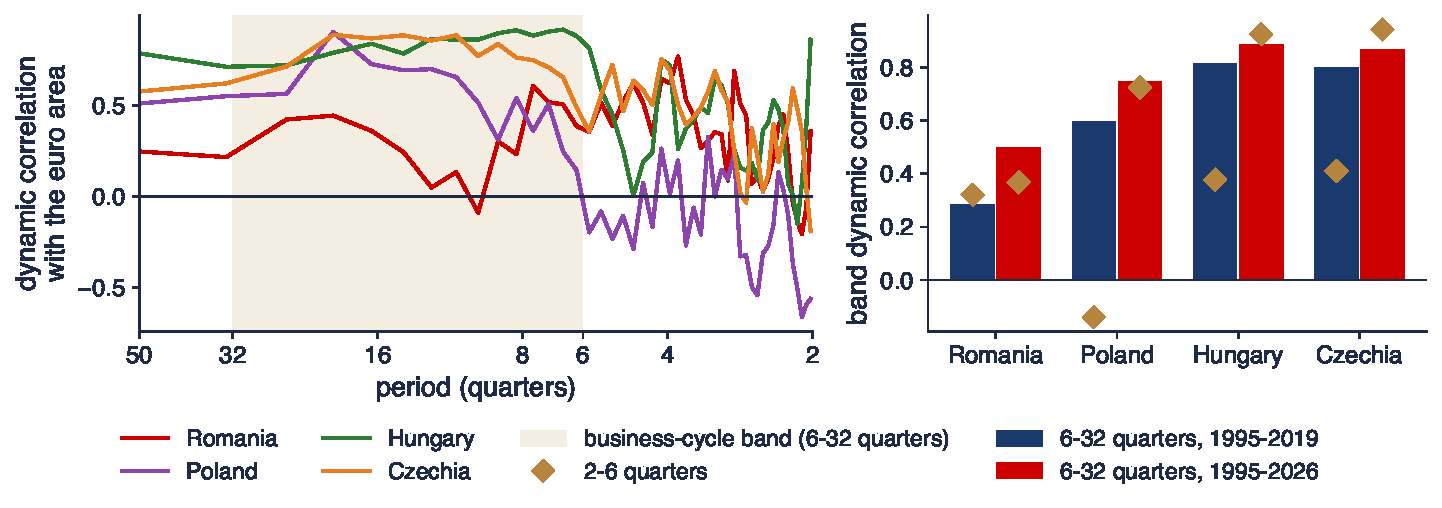
\includegraphics[width=0.97\textwidth,height=0.48\textheight,keepaspectratio]{ats_ch11_dyncorr.pdf}
\end{center}
\vspace{-0.25cm}
\begin{itemize}
    \item Creșterea trimestrială a PIB, multitaper $NW = 3$; stînga: $\rho(\omega)$ pentru 1995--2019; dreapta: mediile pe banda de 6--32 de trimestre (bare) și 2--6 trimestre (romburi), fără și cu 2020--2026
\end{itemize}
\quantlet{ATS\_ch11\_cross\_spectrum}{\qlurl{ATS_ch11_cross_spectrum}}
\end{frame}

\begin{frame}{Interpretarea corelațiilor dinamice}
\itemsize{\small}
\begin{itemize}
    \item Înainte de 2020, corelația dinamică pe banda ciclului economic: Ungaria 0{,}81, Cehia 0{,}80, Polonia 0{,}60, România 0{,}28
    \item Corelația pe termen scurt a Poloniei este \ensuremath{-}0{,}14: creșterea ei s-a mișcat împreună cu zona euro doar prin ciclul economic
    \item Cu 2020--2026 toate valorile cresc (România 0{,}50, Polonia 0{,}75): trimestrul pandemiei domină orice periodogramă încrucișată
    \item Raportați sincronizarea cu și fără șocurile comune extreme; spectrele robuste (trunchiate sau pe ranguri) sînt o temă de cercetare
\end{itemize}
\end{frame}

\begin{frame}{Recapitulare: filtre și ciclul economic}
\itemsize{\small}
\begin{itemize}
    \item Un ciclu este definit de un cîștig: HP este trece-sus, BK și CF aproximează un filtru trece-bandă, filtrul de regresie al lui Hamilton nu este niciunul
    \item HP creează dintr-un mers aleator un ciclu de 30 de trimestre și nu este fiabil în timp real
    \item România este sincronizată cu zona euro ca moment din 2010, cu o amplitudine mai mare
\end{itemize}
\end{frame}


%=============================================================================
\section{Spectre care se schimbă în timp}
%=============================================================================

\begin{frame}{Spectre evolutive și staționaritate locală}
\itemsize{\small}
\begin{itemize}
    \item \refPri: $X_t = \int A_t(\omega)e^{i\omega t}\,dZ(\omega)$, cu o amplitudine $A_t(\omega)$ care se schimbă lent; \textbf{spectrul evolutiv} $f_t(\omega) = |A_t(\omega)|^2f(\omega)$
    \item \refDah: procese \textbf{local staționare} $X_{t,T}$, cu $A(t/T, \omega)$ netedă în timpul rescalat $u = t/T$: un spectru variabil în timp $f(u, \omega)$ care se poate estima consistent
    \begin{itemize}
        \item estimatorul: un spectru pe o fereastră mobilă (transformata Fourier pe termen scurt, spectrograma), cu taper
    \end{itemize}
    \item \textbf{Principiul incertitudinii}: o fereastră de lungime $L$ separă frecvențele doar pînă la circa $1/L$; ferestrele lungi estompează timpul, cele scurte estompează frecvența
    \item Wavelets (secțiunile următoare) lasă lungimea ferestrei să varieze cu frecvența: scurtă pentru frecvențele înalte, lungă pentru cele joase
\end{itemize}
\end{frame}

\begin{frame}{Un spectru care alunecă}
\itemsize{\footnotesize}
\begin{center}
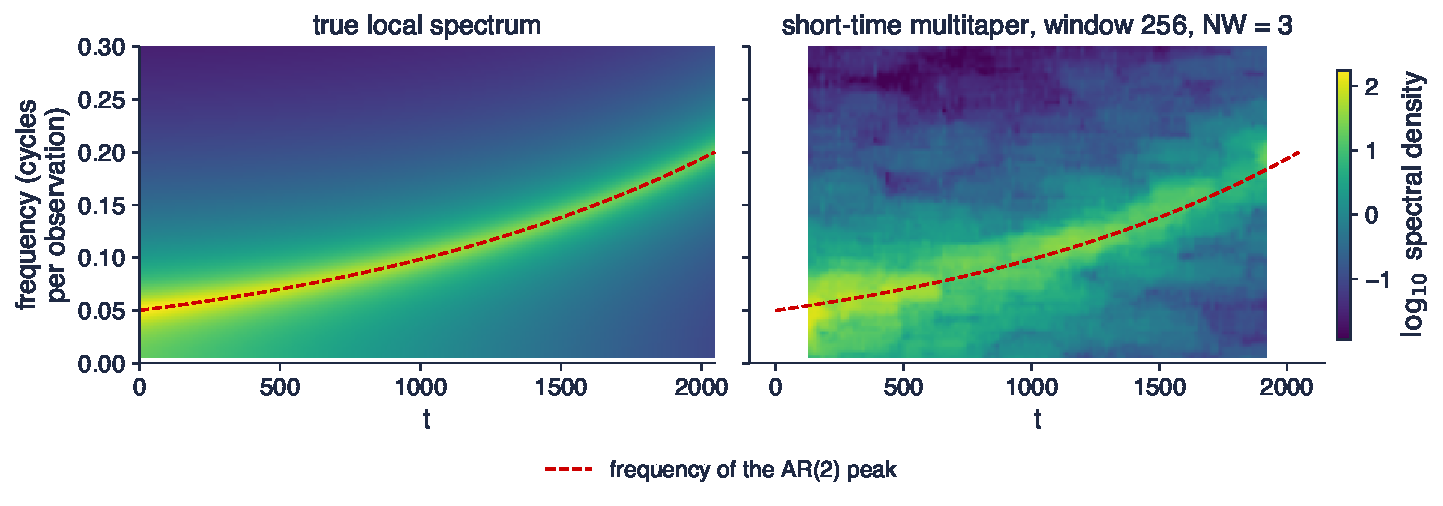
\includegraphics[width=0.97\textwidth,height=0.5\textheight,keepaspectratio]{ats_ch11_spectrogram.pdf}
\end{center}
\vspace{-0.25cm}
\begin{itemize}
    \item $X_t = 2r\cos(\theta_t)X_{t-1} - r^2X_{t-2} + \varepsilon_t$, $r = 0{,}95$, perioada vîrfului trece de la 20 la 5 pe 2048 de observații; multitaper pe ferestre de 256 (pas 16)
\end{itemize}
\quantlet{ATS\_ch11\_evolutionary}{\qlurl{ATS_ch11_evolutionary}}
\end{frame}

\begin{frame}{Interpretarea spectrogramei}
\itemsize{\small}
\begin{itemize}
    \item Spectrograma urmărește vîrful care se deplasează: un singur spectru al întregului eșantion ar arăta o bandă estompată de la 0,05 la 0,2 cicluri
    \item Rezoluția $2NW/L = 0{,}023$ cicluri: bună la frecvențe înalte, grosieră pentru perioadele lungi de la început
    \item Primele și ultimele 128 de observații nu au estimare: orice metodă timp--frecvență pierde marginile (conul de influență al wavelets)
    \item Exemple economice: lungimea variabilă a ciclului economic, scurtarea ciclurilor de tranzacționare, schimbări de regim în volatilitate
\end{itemize}
\end{frame}

\begin{frame}{Analiza spectrului singular pe un slide}
\itemsize{\small}
\begin{itemize}
    \item Scufundăm $x_1, \dots, x_n$ în matricea traiectoriilor (Hankel) $\mathbf X$, de dimensiune $L \times (n - L + 1)$; descompunerea SVD $\mathbf X = \sum_i\sigma_i\mathbf u_i\mathbf v_i'$ \refVG
    \item Grupăm tripletele proprii (tendința: $\mathbf u_i$ care variază lent; oscilațiile: perechi cu $\sigma_i$ egale și sinusoide decalate) și reconstruim fiecare grup prin medierea antidiagonalelor
    \item O bază adaptată la date în locul sinusoidelor sau al wavelets fixe; fără model și fără ipoteza de staționaritate; inferența este mai puțin dezvoltată
    \item O schiță de cod (\texttt{ssa}) se află în nucleul Quantlet al capitolului; este un reper natural pentru analiza multirezoluție wavelet
\end{itemize}
\end{frame}

\begin{frame}{Recapitulare: spectre care se schimbă în timp}
\itemsize{\small}
\begin{itemize}
    \item Priestley și Dahlhaus dau un sens unui spectru variabil în timp
    \item O fereastră fixă schimbă rezoluția în timp pe rezoluția în frecvență
    \item Wavelets adaptează fereastra la frecvență; SSA adaptează baza la date
\end{itemize}
\end{frame}


%=============================================================================
\section{Wavelets: descompunerea pe scale}
%=============================================================================

\begin{frame}{De la sinusoide la wavelets}
\itemsize{\small}
\begin{columns}[T]
\begin{column}{0.3\textwidth}
\centering
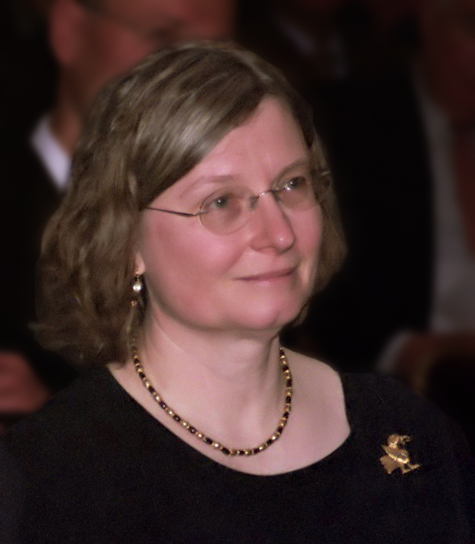
\includegraphics[height=0.4\textheight]{ch11_daubechies_2005.jpg}\\[1mm]
\imgcap{Ingrid Daubechies, 2005}
\imgcredit{https://commons.wikimedia.org/wiki/File:Ingrid_Daubechies_(2005)_(cropped).jpg}{Foto: lucrarea autorului încărcării (2005); domeniu public; Wikimedia Commons}
\end{column}
\begin{column}{0.68\textwidth}
\begin{itemize}
    \item Un \textbf{wavelet} $\psi$: $\int\psi = 0$, $\int\psi^2 = 1$, localizat în timp și în frecvență; admisibil dacă $C_\psi = \int|\hat\psi(\omega)|^2/|\omega|\,d\omega < \infty$ \refGM
    \item CWT: $W(s, \tau) = \int x(t)\frac{1}{\sqrt s}\psi^*\big(\frac{t - \tau}{s}\big)dt$; scala $s$ este invers legată de frecvență
    \item Wavelets ortonormate cu suport compact \refDau{} și algoritmul piramidal \refMal{} dau DWT: $n$ coeficienți pentru $n$ observații
    \item În economie și finanțe: \refCro; \refGSWb; \refACS
\end{itemize}
\end{column}
\end{columns}
\end{frame}

\begin{frame}{DWT, MODWT și analiza multirezoluție}
\itemsize{\small}
\begin{itemize}
    \item Filtre: de scalare $g_l$ (trece-jos), wavelet $h_l = (-1)^lg_{L-1-l}$ (trece-sus); Haar $L = 2$, Daubechies cel mai puțin asimetric LA(8) $L = 8$ \refPWb
    \begin{itemize}
        \item nivelul $j$ captează perioadele $[2^j, 2^{j+1}]$: o bandă de o \textbf{octavă}; $J$ niveluri plus o componentă netedă
    \end{itemize}
    \item \textbf{MODWT}: fără eșantionare redusă; filtre rescalate $\tilde h = h/\sqrt2$, $\tilde g = g/\sqrt2$; $\tilde W_{j,t} = \sum_l\tilde h_{j,l}X_{t-l \bmod n}$
    \begin{itemize}
        \item orice mărime a eșantionului, invariantă la translații (mutarea datei de început nu schimbă coeficienții), $J \times n$ coeficienți, energia se conservă: $\|X\|^2 = \sum_j\|\tilde W_j\|^2 + \|\tilde V_J\|^2$
    \end{itemize}
    \item \textbf{MRA}: $X_t = \sum_{j=1}^J\mathcal D_{j,t} + \mathcal S_{J,t}$, fiecare detaliu $\mathcal D_j$ fiind inversa MODWT a nivelului $j$; fără defazaj, aliniat cu datele
    \item Marginile: primii $L_j - 1 = (2^j - 1)(L - 1)$ coeficienți folosesc date de la celălalt capăt (filtrare circulară) și se exclud din estimare
\end{itemize}
\end{frame}

\begin{frame}{Filtre wavelet și wavelet-ul Morlet}
\itemsize{\footnotesize}
\begin{center}
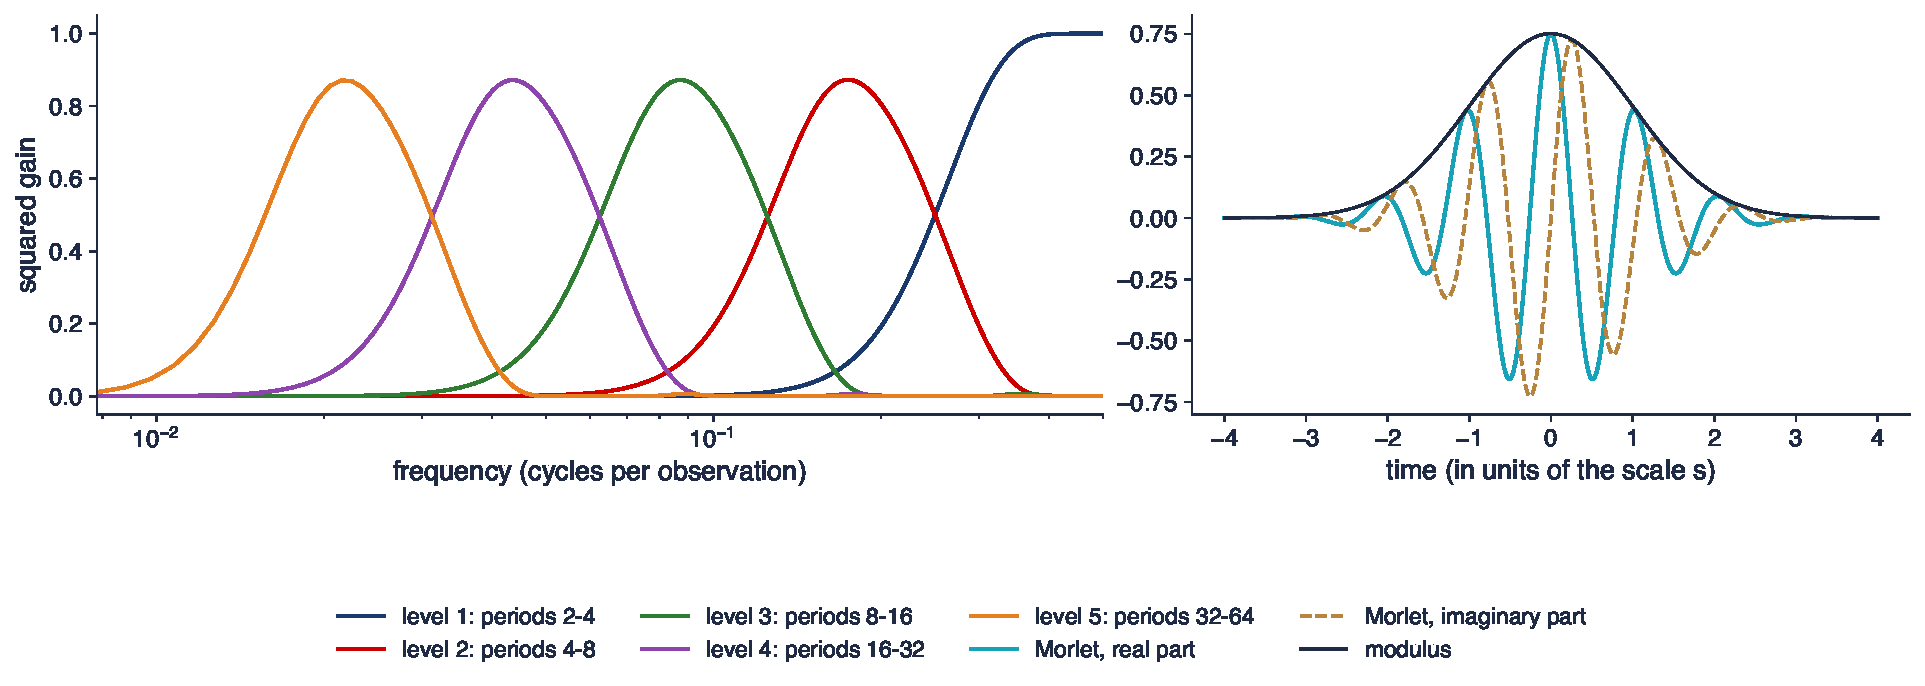
\includegraphics[width=0.97\textwidth,height=0.48\textheight,keepaspectratio]{ats_ch11_wavelets.pdf}
\end{center}
\vspace{-0.25cm}
\begin{itemize}
    \item Stînga: pătratele cîștigurilor filtrelor MODWT LA(8) pentru nivelurile 1--5; dreapta: wavelet-ul Morlet $\psi_0(\eta) = \pi^{-1/4}e^{i\omega_0\eta}e^{-\eta^2/2}$, $\omega_0 = 6$
\end{itemize}
\quantlet{ATS\_ch11\_wavelets}{\qlurl{ATS_ch11_wavelets}}
\end{frame}

\begin{frame}{Interpretarea filtrelor wavelet}
\itemsize{\small}
\begin{itemize}
    \item Fiecare nivel MODWT este un filtru trece-bandă aproximativ pentru o octavă; benzile se suprapun, deci scurgerea între niveluri vecine face parte din construcție
    \item Lățimea benzii crește cu frecvența: rezoluție fină în frecvență pentru ciclurile lungi, rezoluție fină în timp pentru cele scurte
    \item Morlet este complex: modulul dă amplitudinea, argumentul dă faza; perioada Fourier $= 1{,}033\times$ scala pentru $\omega_0 = 6$
    \item Filtrele ortonormate (MODWT) servesc descompunerii varianței și corelației pe scale; CWT Morlet servește hărților timp--frecvență și fazei
\end{itemize}
\end{frame}

\begin{frame}{Randamentul BET descompus pe scale}
\itemsize{\footnotesize}
\begin{center}
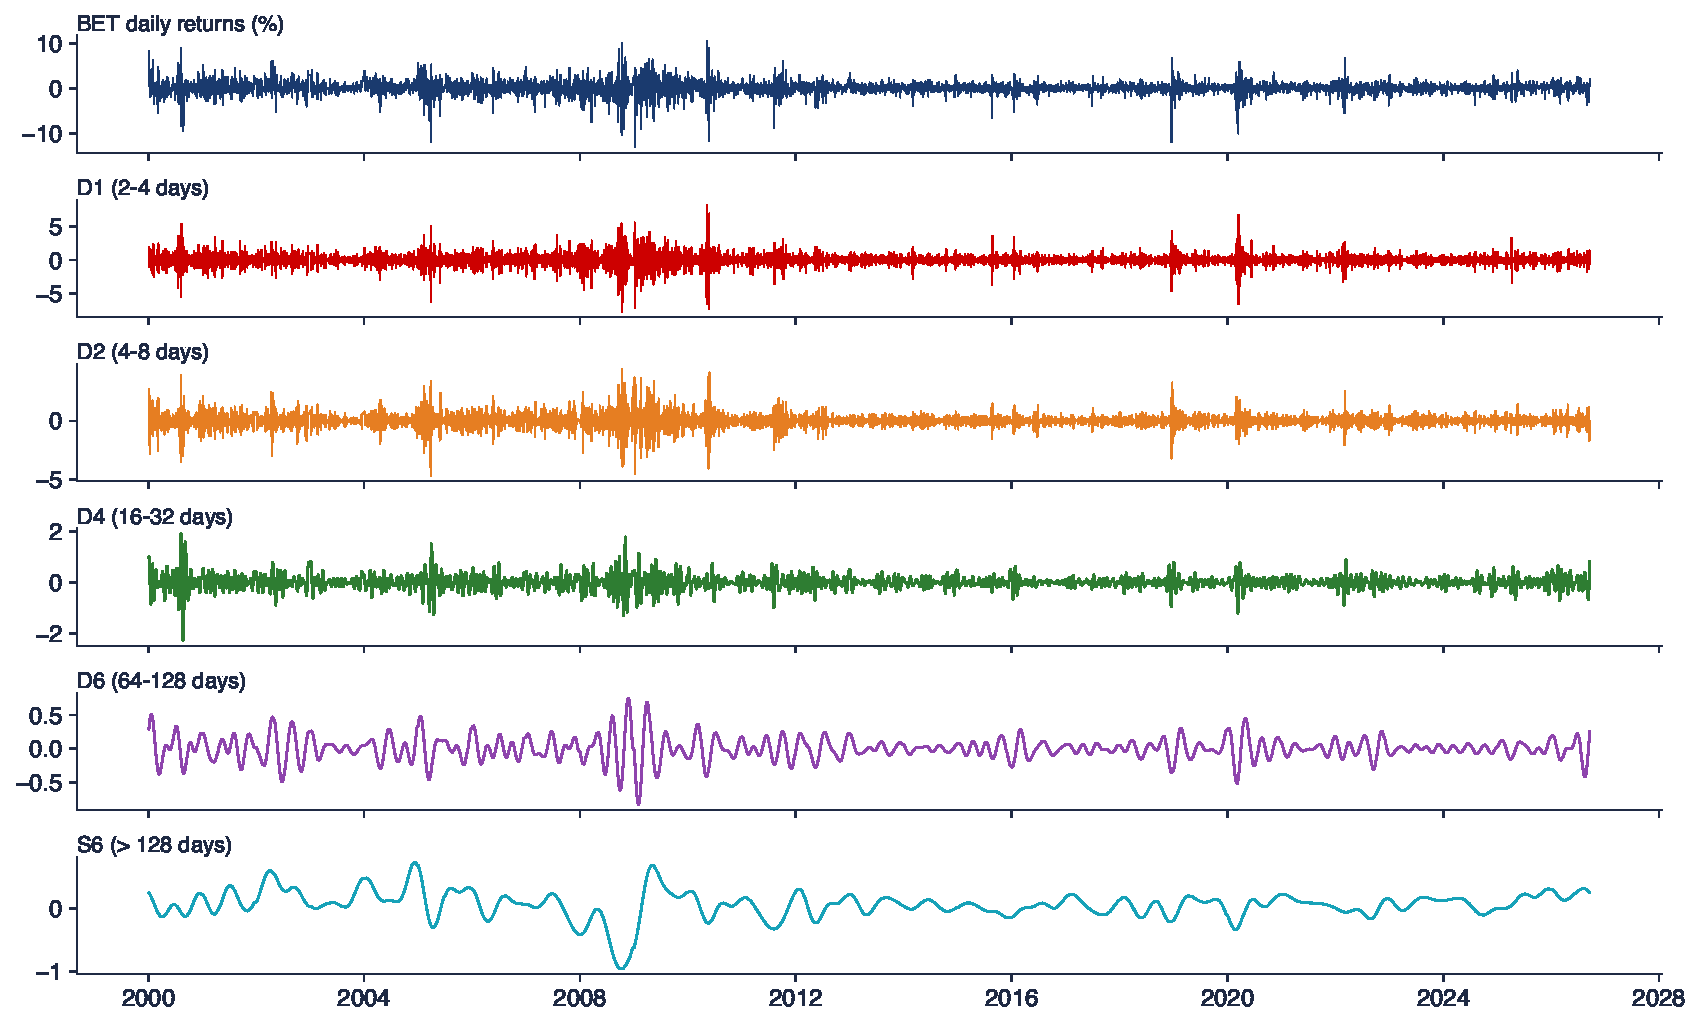
\includegraphics[width=0.97\textwidth,height=0.68\textheight,keepaspectratio]{ats_ch11_mra.pdf}
\end{center}
\vspace{-0.25cm}
\begin{itemize}
    \item Analiza multirezoluție MODWT, LA(8), $J = 6$, randamentele zilnice BET 2000--2026 (6\,670 de zile); patru dintre cele șase detalii și componenta netedă
\end{itemize}
\quantlet{ATS\_ch11\_wavelets}{\qlurl{ATS_ch11_wavelets}}
\end{frame}

\begin{frame}{Interpretarea analizei multirezoluție}
\itemsize{\small}
\begin{itemize}
    \item Ponderile energiei pe nivelurile 1--6: 43{,}0; 26{,}6; 15{,}0; 6{,}8; 3{,}5; 2{,}3\%; un zgomot alb ar da 50{,}0; 25{,}0; 12{,}5; 6{,}2; 3{,}1; 1{,}6\%
    \item Mai puțină energie la scala cea mai scurtă și mai multă la scalele lungi decît un zgomot alb: autocorelația pozitivă a randamentelor BET la orizonturi scurte
    \item Volatility clustering apare la toate scalele în 2008 și 2020, dar componentele lente ($\mathcal D_6$, $\mathcal S_6$) se mișcă doar în criza din 2008--2009
    \item Detaliile se adună exact la serie: o descompunere fără pierderi și fără defazaj
\end{itemize}
\end{frame}

\begin{frame}{Varianța, corelația și beta wavelet pe scale}
\itemsize{\small}
\begin{itemize}
    \item \textbf{Varianța wavelet} $\nu_X^2(\tau_j) = \Var\tilde W_{j,t}$; $\sum_j\nu^2_X(\tau_j) = \Var X$: o versiune pe octave a spectrului \refPer
    \begin{itemize}
        \item estimatorul nedeplasat: media lui $\tilde W^2_{j,t}$ pe cei $M_j = n - L_j + 1$ coeficienți din afara marginilor; $\eta\hat\nu^2/\nu^2 \approx \chi^2_\eta$, $\eta = \max(M_j/2^j, 1)$
        \item zgomot alb: $\nu^2(\tau_j) = \sigma^2/2^j$, se înjumătățește la fiecare nivel
    \end{itemize}
    \item \textbf{Corelația wavelet} $\rho_{XY}(\tau_j) = \Cov(\tilde W^X_j, \tilde W^Y_j)/(\nu_X\nu_Y)$, intervalul $\tanh\big(\tanh^{-1}\hat\rho \pm z/\sqrt{M_j/2^j - 3}\big)$ \refWGP
    \item \textbf{Beta wavelet} $\beta(\tau_j) = \Cov(\tilde W^r_j, \tilde W^m_j)/\Var\tilde W^m_j$: riscul sistematic pe orizonturi de investiție \refGSW
    \item Mărimea efectivă a eșantionului se înjumătățește la fiecare nivel: estimările pe scale lungi sînt largi chiar și cu 25 de ani de date zilnice
\end{itemize}
\end{frame}

\begin{frame}{Varianța wavelet a trei indici bursieri}
\itemsize{\footnotesize}
\begin{center}
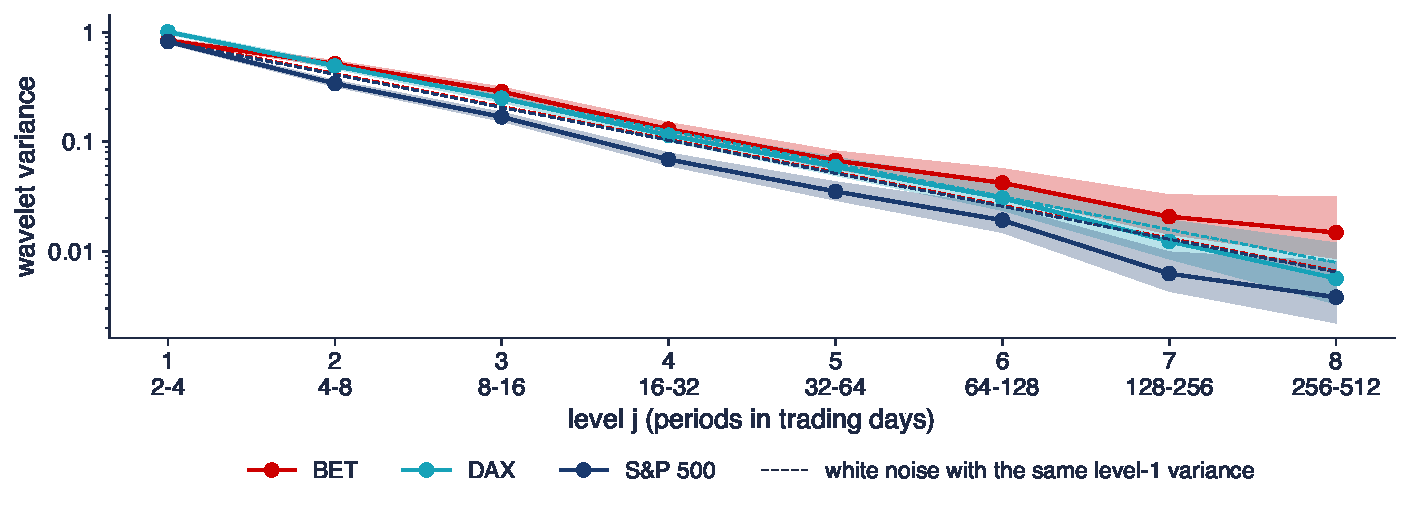
\includegraphics[width=0.97\textwidth,height=0.5\textheight,keepaspectratio]{ats_ch11_wvar.pdf}
\end{center}
\vspace{-0.25cm}
\begin{itemize}
    \item Randamente logaritmice zilnice 2000--2026, MODWT LA(8), nivelurile 1--8 cu intervale de 95\%; linii întrerupte: zgomot alb cu aceeași varianță la nivelul 1
\end{itemize}
\quantlet{ATS\_ch11\_wavelets}{\qlurl{ATS_ch11_wavelets}}
\end{frame}

\begin{frame}{Interpretarea varianțelor wavelet}
\itemsize{\small}
\begin{itemize}
    \item Raportul dintre varianța de la nivelul 6 (64--128 de zile) și linia zgomotului alb: BET 1{,}60, DAX 0{,}97, S\&P 500 0{,}75
    \item BET are mai multă varianță pe orizonturi lungi decît implică varianța zilnică (nivelul 8: 2{,}25): momentum, o piață mică; S\&P 500 are mai puțină (0{,}59): revenirea la medie a mișcărilor zilnice
    \item Este testul raportului varianțelor pentru eficiența pieței, făcut scală cu scală, cu intervale valide
    \item Riscul măsurat pe date zilnice și scalat cu $\sqrt{h}$ subestimează riscul BET pe orizonturi lungi
\end{itemize}
\end{frame}

\begin{frame}{Co-mișcarea pe scale: BET, DAX și S\&P 500}
\itemsize{\footnotesize}
\begin{center}
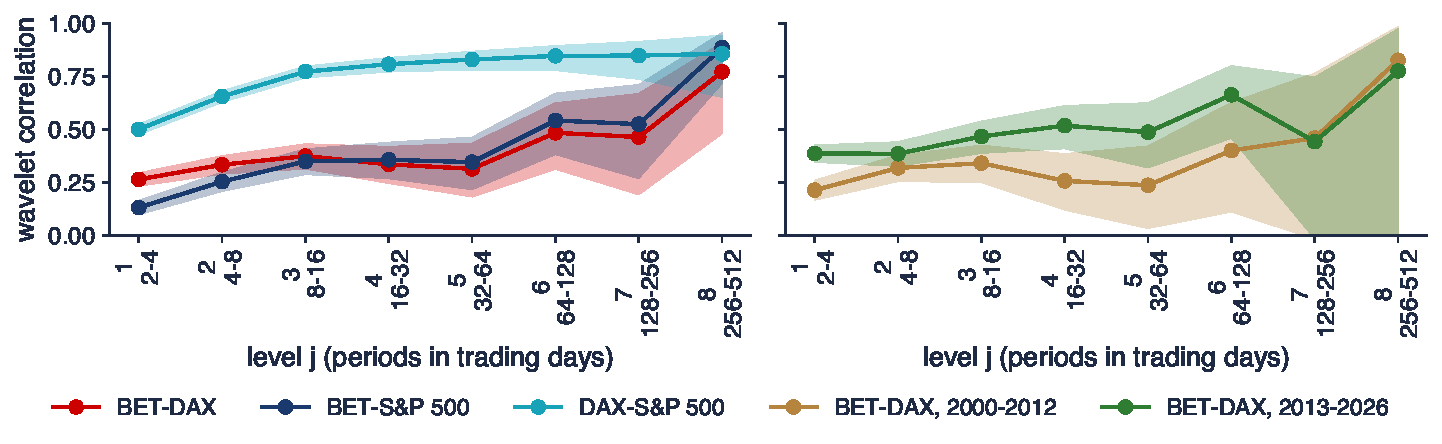
\includegraphics[width=0.97\textwidth,height=0.5\textheight,keepaspectratio]{ats_ch11_wcorr.pdf}
\end{center}
\vspace{-0.25cm}
\begin{itemize}
    \item Randamente zilnice în 6\,433 de zile comune de tranzacționare, MODWT LA(8); stînga: trei perechi, 2000--2026; dreapta: BET--DAX în două jumătăți; intervale Fisher-$z$ de 95\%
\end{itemize}
\quantlet{ATS\_ch11\_wavelets}{\qlurl{ATS_ch11_wavelets}}
\end{frame}

\begin{frame}{Interpretarea corelațiilor wavelet}
\itemsize{\footnotesize}
\begin{itemize}
    \item BET--DAX crește de la 0{,}26 (2--4 zile) la 0{,}77 (256--512 zile); corelația zilnică (0{,}31) subestimează integrarea pe termen lung
    \item BET--S\&P 500 la nivelul 1 este doar 0{,}13, DAX--S\&P 500 0{,}50: New York închide după Europa, deci co-mișcarea zilnică apare cu o zi întîrziere; dispare la scale mai lungi
    \item BET--DAX la 8--16 zile: 0{,}34 în 2000--2012 față de 0{,}47 în 2013--2026 (nivelul 3): integrarea a crescut la scale scurte și medii
    \item Beta wavelet a BET față de DAX: 0{,}24 la nivelul 1, 0{,}56 la nivelul 6: beneficiul diversificării prin BET scade cu orizontul (\refGSW; \refRN)
\end{itemize}
\end{frame}

\begin{frame}{Recapitulare: wavelets: descompunerea pe scale}
\itemsize{\small}
\begin{itemize}
    \item MODWT împarte varianța și covarianța pe benzi de o octavă, pentru orice $n$ și fără defazaj
    \item Varianța wavelet este un test al raportului varianțelor scală cu scală; corelația și beta wavelet arată integrarea pe orizonturi
    \item Excludeți coeficienții de margine și folosiți grade de libertate echivalente pentru intervale
\end{itemize}
\end{frame}


%=============================================================================
\section{Co-mișcarea timp--frecvență: coerența wavelet}
%=============================================================================

\begin{frame}{Transformata Morlet și semnificația ei}
\itemsize{\small}
\begin{itemize}
    \item \refTC: $W_n(s) = \sum_kx\hat{}_k\hat\psi^*(s\omega_k)e^{i\omega_kn\delta t}$ prin FFT; scalele $s_j = s_02^{j\delta j}$; puterea wavelet $|W_n(s)|^2$
    \begin{itemize}
        \item \textbf{conul de influență} (COI): zona în care wavelet-ul de scală $s$ atinge marginea, la mai puțin de $\sqrt2\,s$ de oricare capăt; rezultatele de acolo sînt deplasate
    \end{itemize}
    \item Ipoteza nulă de zgomot roșu (AR(1) cu autocorelația de ordinul 1 egală cu $a$): $|W_n(s)|^2/\sigma^2 \sim P_k\chi^2_2/2$, $P_k = (1 - a^2)/(1 + a^2 - 2a\cos(2\pi k/N))$ la frecvența scalei $s$
    \begin{itemize}
        \item spectrul wavelet global $\bar W^2(s) = \frac1n\sum_n|W_n(s)|^2$: un spectru Fourier netezit cu $\nu = 2\sqrt{1 + (n\delta t/(2{,}32s))^2}$ grade de libertate
    \end{itemize}
    \item Rectificați puterea prin $1/s$ cînd comparați scalele \refLLW; testul punctual se aplică în mii de puncte: așteptați 5\% zone false \refMK
\end{itemize}
\end{frame}

\begin{frame}{Puterea wavelet a BET}
\itemsize{\footnotesize}
\begin{center}
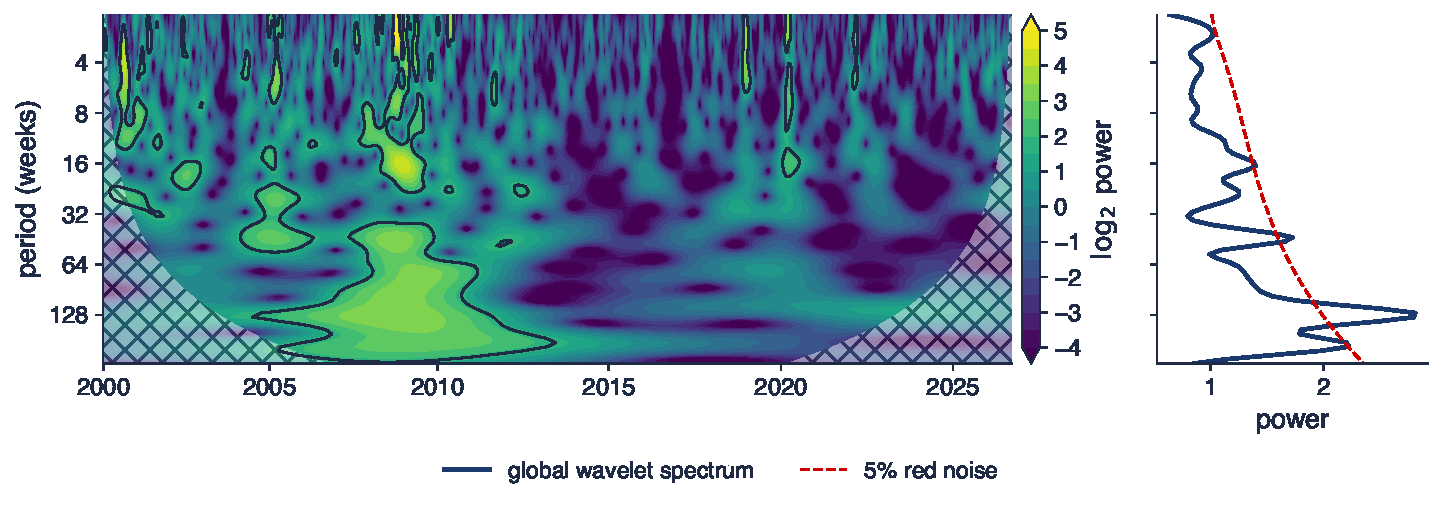
\includegraphics[width=0.97\textwidth,height=0.48\textheight,keepaspectratio]{ats_ch11_cwt_bet.pdf}
\end{center}
\vspace{-0.25cm}
\begin{itemize}
    \item Randamente săptămînale BET (standardizate), 1\,379 de săptămîni 2000--2026, Morlet $\omega_0 = 6$, $\delta j = 1/12$; contururi negre: testul de 5\% față de zgomotul roșu; hașurat: conul de influență; dreapta: spectrul wavelet global
\end{itemize}
\quantlet{ATS\_ch11\_wavelet\_coherence}{\qlurl{ATS_ch11_wavelet_coherence}}
\end{frame}

\begin{frame}{Interpretarea puterii wavelet}
\itemsize{\small}
\begin{itemize}
    \item Puterea maximă la perioada de 2{,}6 săptămîni, la 17 octombrie 2008: săptămînile Lehman; putere semnificativă în 2007--2011 la perioade de 32--128 de săptămîni
    \item Autocorelația de ordinul 1 este 0{,}04: ipoteza nulă de zgomot roșu este aproape albă; 11\% din aria fiabilă este semnificativă la 5\%
    \item Puterea în randamente este varianță, nu un ciclu: harta arată cînd s-a concentrat volatilitatea și la ce orizonturi
    \item Spectrul global rămîne în interiorul benzii zgomotului roșu: niciun ciclu persistent în randamentele BET, cum prezice eficiența pieței
\end{itemize}
\end{frame}

\begin{frame}{Coerența și faza wavelet}
\itemsize{\small}
\begin{itemize}
    \item Transformata wavelet încrucișată $W^{xy}_n(s) = W^x_n(s)W^{y*}_n(s)$; \textbf{coerența wavelet pătratică} \refTW, \refGMJ:
    \begin{itemize}
        \item $R^2_n(s) = \dfrac{|\mathcal S(s^{-1}W^{xy}_n(s))|^2}{\mathcal S(s^{-1}|W^x_n(s)|^2)\,\mathcal S(s^{-1}|W^y_n(s)|^2)}$, $\mathcal S$ = netezire gaussiană în timp (lățime $s$) și o medie pe 0,6 octave în scală
        \item fără netezire $R^2 \equiv 1$, ca pentru coerența brută: netezirea o face un estimator
    \end{itemize}
    \item Faza $\arg\mathcal S(s^{-1}W^{xy})$: săgeți spre dreapta = în fază, spre stînga = în antifază, în sus = $x$ conduce; avansul în timp = faza $\times$ perioada$/2\pi$
    \item Semnificația prin \textbf{Monte Carlo} \refGMJ: perechi de serii AR(1) independente cu autocorelațiile de ordinul 1 ale datelor; percentila 95 a lui $R^2$ la fiecare scală
    \item Extensii: coerența wavelet parțială și multiplă, diferențe de fază cu benzi de încredere \refACS; politica monetară \refAAS; energie \refVB
\end{itemize}
\end{frame}

\begin{frame}{BET și DAX în timp și frecvență}
\itemsize{\footnotesize}
\begin{center}
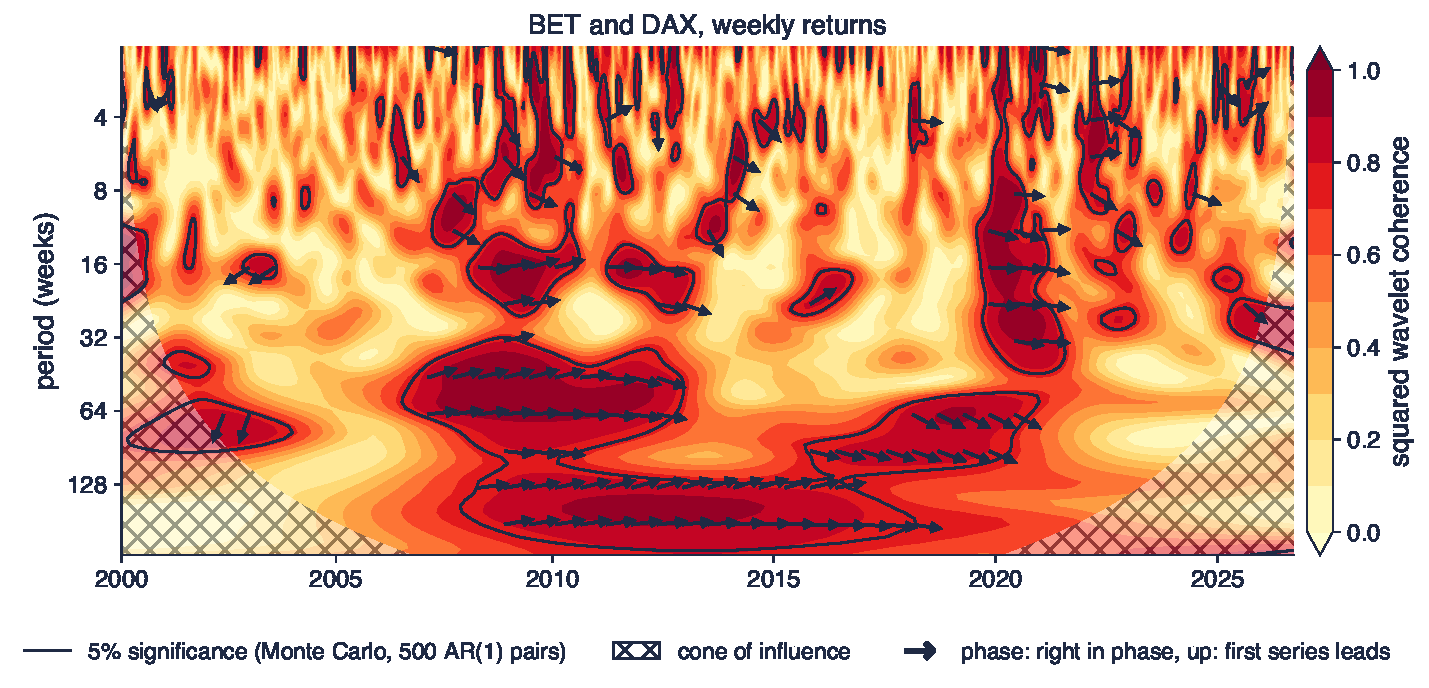
\includegraphics[width=0.97\textwidth,height=0.52\textheight,keepaspectratio]{ats_ch11_wtc_bet_dax.pdf}
\end{center}
\vspace{-0.25cm}
\begin{itemize}
    \item Randamente săptămînale 2000--2026; contururi: semnificația de 5\% din 500 de perechi AR(1); săgeți doar unde coerența este semnificativă
\end{itemize}
\quantlet{ATS\_ch11\_wavelet\_coherence}{\qlurl{ATS_ch11_wavelet_coherence}}
\end{frame}

\begin{frame}{Interpretarea coerenței BET--DAX}
\itemsize{\footnotesize}
\begin{itemize}
    \item 23\% din aria fiabilă este semnificativă (percentila 95 sub ipoteza nulă: 7{,}7\%): co-mișcarea este reală, dar concentrată
    \item $R^2$ mediu la 8--64 de săptămîni: 0{,}37 în 2000--2006, 0{,}76 în 2008--2009, 0{,}36 în 2014--2019, 0{,}77 în 2020--iunie 2021
    \item Faza aproape zero în crize (0{,}03 rad în 2008--2009), negativă înainte de 2007 (\ensuremath{-}0{,}97 rad): DAX conducea BET cu cîteva săptămîni cînd piața de la București era tînără
    \item Crizele cresc coerența: este contagiune sau doar volatilitate mai mare? Corelațiile cresc mecanic cu volatilitatea \refFR, la fel și $R^2$
\end{itemize}
\end{frame}

\begin{frame}{BET și S\&P 500 în timp și frecvență}
\itemsize{\footnotesize}
\begin{center}
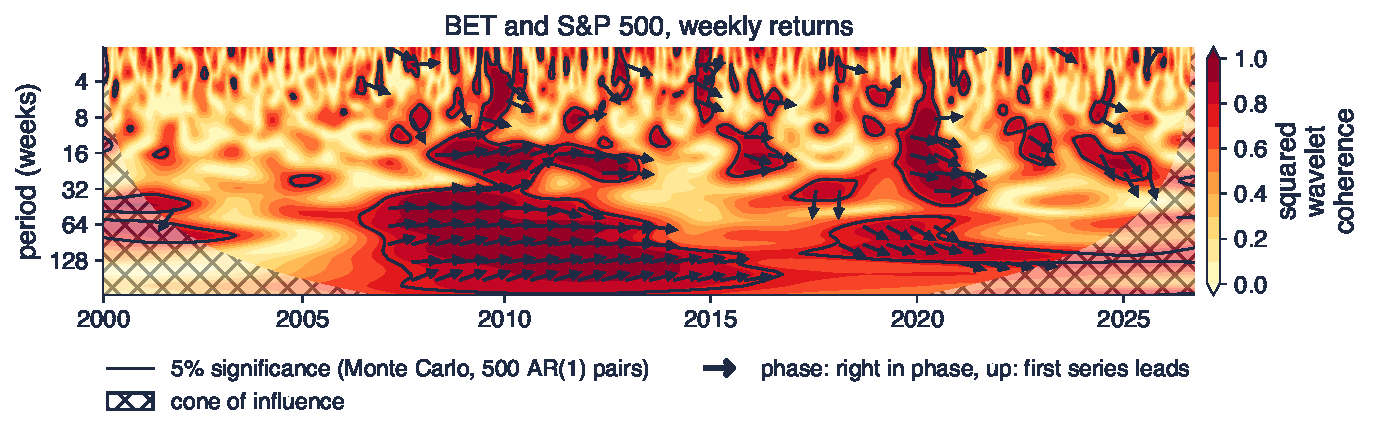
\includegraphics[width=0.97\textwidth,height=0.52\textheight,keepaspectratio]{ats_ch11_wtc_bet_spx.pdf}
\end{center}
\vspace{-0.25cm}
\begin{itemize}
    \item Randamente săptămînale 2000--2026; semnificația Monte Carlo ca mai înainte
\end{itemize}
\quantlet{ATS\_ch11\_wavelet\_coherence}{\qlurl{ATS_ch11_wavelet_coherence}}
\end{frame}

\begin{frame}{Interpretarea coerenței BET--S\&P 500}
\itemsize{\small}
\begin{itemize}
    \item Aria semnificativă 26\% (percentila 95 sub ipoteza nulă: 7{,}7\%); $R^2$ la 8--64 de săptămîni 0{,}76 în 2008--2009 și 0{,}48 în 2014--2019
    \item În 2000--2006 faza este \ensuremath{-}1{,}24 rad: S\&P 500 conducea cu circa o cincime din ciclu; în crize piețele se mișcă în fază
    \item Datele săptămînale elimină decalajul de o zi din corelația wavelet zilnică: alegerea frecvenței datelor contează pentru afirmațiile despre decalaje
    \item Imaginea noastră confirmă evidența internațională: co-mișcarea este cea mai puternică la frecvențe joase și în crize \refRN
\end{itemize}
\end{frame}

\begin{frame}{Petrolul și acțiunile}
\itemsize{\footnotesize}
\begin{center}
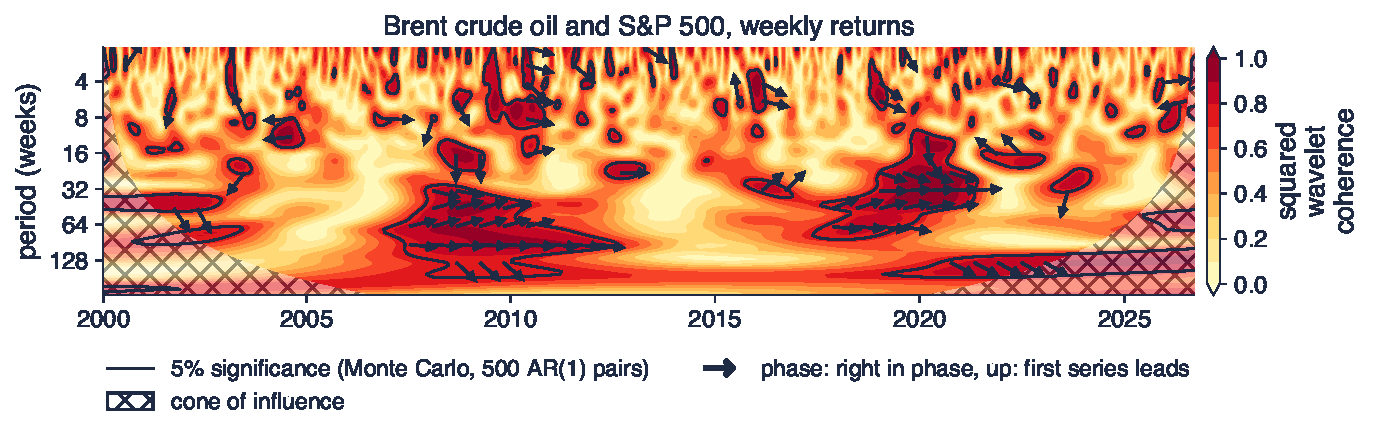
\includegraphics[width=0.97\textwidth,height=0.52\textheight,keepaspectratio]{ats_ch11_wtc_oil.pdf}
\end{center}
\vspace{-0.25cm}
\begin{itemize}
    \item Randamente săptămînale ale petrolului Brent (FRED) și ale S\&P 500, 2000--2026; semnificația Monte Carlo din 500 de perechi AR(1)
\end{itemize}
\quantlet{ATS\_ch11\_wavelet\_coherence}{\qlurl{ATS_ch11_wavelet_coherence}}
\end{frame}

\begin{frame}{Interpretarea coerenței petrol--acțiuni}
\itemsize{\footnotesize}
\begin{itemize}
    \item Aria semnificativă 15\% (percentila 95 sub ipoteza nulă: 7{,}1\%): petrolul și acțiunile sînt legate doar în anumite episoade
    \item Înainte de 2007: $R^2$ 0{,}41, cu faza \ensuremath{-}1{,}86 rad, nici în fază, nici în antifază: o legătură slabă, cu decalaj; 2008--2010: 0{,}70, în fază (\ensuremath{-}0{,}09 rad): un șoc comun de cerere
    \item 2020--2021: 0{,}58 în fază; 2022--2023: faza \ensuremath{-}2{,}31 rad, mai aproape de antifază: șocul prețurilor energiei din timpul războiului din Ucraina
    \item Semnul legăturii petrol--acțiuni depinde de tipul de șoc \refKP; faza wavelet arată schimbarea fără să o identifice
\end{itemize}
\end{frame}

\begin{frame}{Inflația în România și în zona euro}
\itemsize{\footnotesize}
\begin{center}
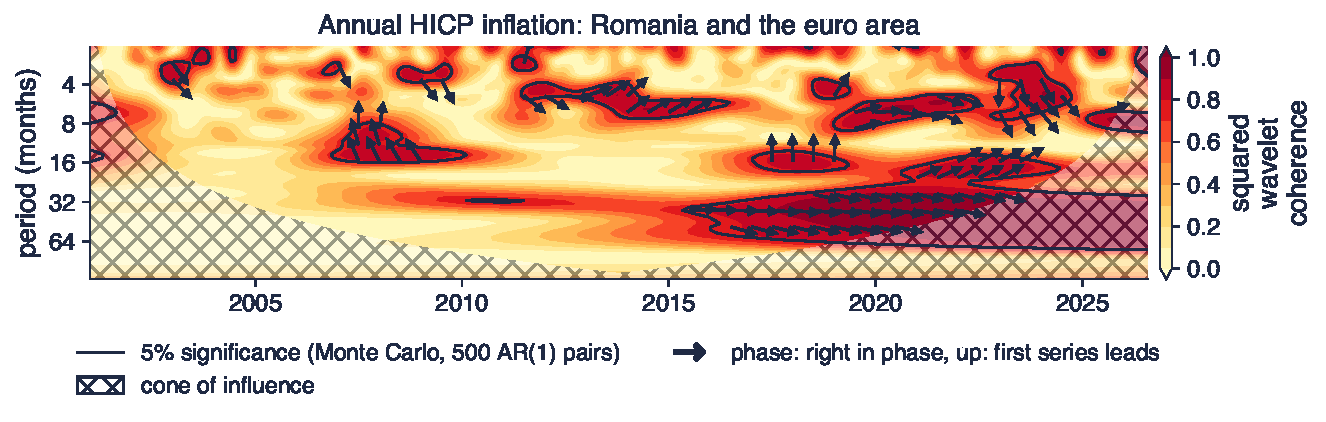
\includegraphics[width=0.97\textwidth,height=0.5\textheight,keepaspectratio]{ats_ch11_wtc_infl_ro.pdf}
\end{center}
\vspace{-0.25cm}
\begin{itemize}
    \item Inflația anuală HICP (lunar), ianuarie 2001 -- august 2026; semnificația Monte Carlo față de perechi AR(1) cu autocorelația de ordinul 1 egală cu 0{,}97
\end{itemize}
\quantlet{ATS\_ch11\_wavelet\_coherence}{\qlurl{ATS_ch11_wavelet_coherence}}
\end{frame}

\begin{frame}{Interpretarea co-mișcării inflației}
\itemsize{\footnotesize}
\begin{itemize}
    \item România--zona euro: $R^2$ la 24--64 de luni 0{,}23 în 2002--2012, 0{,}85 din 2015; aria semnificativă 17\% (percentila 95 sub ipoteza nulă: 8{,}7\%)
    \item Polonia: 0{,}29 și 0{,}91; corelații simple 0{,}34 (România) și 0{,}86 (Polonia): dezinflația României pînă în 2012 a fost internă, ciclul de după 2015 este comun
    \item Creșterea din 2021--2024, 12--48 de luni: $R^2$ 0{,}78, faza 0{,}14 rad: niciun avans detectabil, un șoc energetic comun
    \item Ratele anuale se suprapun pe douăsprezece luni: perioadele scurte sînt netezite prin construcție; doar ciclurile mai lungi de un an sînt informative
\end{itemize}
\end{frame}

\begin{frame}{Recapitulare: coerența wavelet}
\itemsize{\small}
\begin{itemize}
    \item Coerența wavelet este o coerență locală în timp, netezită; fără netezire este identic egală cu unu
    \item Testați-o prin Monte Carlo față de perechi AR(1); citiți faza doar în zonele semnificative și în afara conului de influență
    \item Co-mișcarea acțiunilor este maximă în crize și pe orizonturi lungi; faza petrol--acțiuni se inversează cu tipul de șoc
\end{itemize}
\end{frame}


%=============================================================================
\section{AI în descoperirea științifică}
%=============================================================================

\begin{frame}{O întrebare deschisă}
\itemsize{\small}
\begin{itemize}
    \item Este creșterea coerenței dintre piețele bursiere în crize contagiune sau efectul mecanic al volatilității mai mari asupra unui $R^2$ local în timp?
    \begin{itemize}
        \item formal: $H_0$: coerența wavelet dintre BET și DAX în ferestrele de criză preînregistrate este egală cu valoarea ei într-un model cu aceleași volatilități variabile în timp și dependență constantă
        \item infirmată dacă coerența din criză depășește percentila 95 a unui bootstrap dintr-un DCC-GARCH cu corelație constantă (\atschlink{https://danpele.github.io/Advanced-Time-Series/RO/Cursuri/capitol8_volatilitate_avansata.pdf}{Capitolul 8}), la scale preînregistrate
    \end{itemize}
    \item De ce contează: diversificarea eșuează tocmai cînd este nevoie de ea; corecția Forbes--Rigobon există pentru corelații, nu și pentru coerența wavelet
    \begin{itemize}
        \item literatura de pornire: \refFR, \refRN, \refMK, \refSch, \refACS
    \end{itemize}
\end{itemize}
\end{frame}

\begin{frame}{Bucla de cercetare cu un asistent AI}
\itemsize{\footnotesize}
\begin{itemize}
    \item Un asistent AI (un LLM precum Claude, ChatGPT, Gemini sau Copilot) accelerează fiecare etapă; Semantic Scholar și Elicit ajută la literatură
    \begin{itemize}
        \item \textbf{literatura}: \aiprompt{Listează articole recenzate din 2009 încoace care testează coerența wavelet dintre piețe bursiere față de o ipoteză nulă cu aceeași volatilitate; dă DOI-urile.} Apoi verificați fiecare DOI pe Crossref
        \item \textbf{ipoteza}: \aiprompt{Derivează deplasarea coerenței wavelet netezite cînd ambele serii au o volatilitate GARCH comună și corelație constantă.}
        \item \textbf{cod și replicare}: cereți operatorul de netezire Grinsted, apoi reproduceți întîi un caz cunoscut (două serii AR(1): 5\% arie semnificativă)
        \item \textbf{critica}: \aiprompt{Joacă rolul unui recenzent ostil: enumeră felurile în care poate apărea o insulă semnificativă de coerență wavelet fără nicio schimbare a dependenței.}
    \end{itemize}
    \item Raportul: ce s-a cerut, ce s-a păstrat, ce s-a respins (AI\_USE.md, AI\_ERRORS.md)
\end{itemize}
\end{frame}

\begin{frame}{Verificări necesare}
\itemsize{\small}
\begin{itemize}
    \item Fiecare referință există și spune ce se afirmă (DOI-ul funcționează, titlul coincide, rezultatul se află în lucrare)
    \item Convențiile: frecvență unghiulară sau cicluri, factorii $2\pi$, perioada $=$ $1{,}033\times$ scala pentru Morlet, convenția de semn a fazei
    \item Coerența este netezită; pragul ei și ipoteza nulă Monte Carlo sînt precizate; nimic nu se interpretează în conul de influență
    \item Semnificația punctuală nu este semnificație pe arii: numărați cîte insule produce ipoteza nulă
    \item Filtre: cîștigul precizat; ciclul în timp real separat de cel final; rezultate cu și fără șocurile comune extreme
\end{itemize}
\end{frame}

\begin{frame}{Mini studiu de caz: cîte insule produce întîmplarea?}
\itemsize{\footnotesize}
\begin{center}
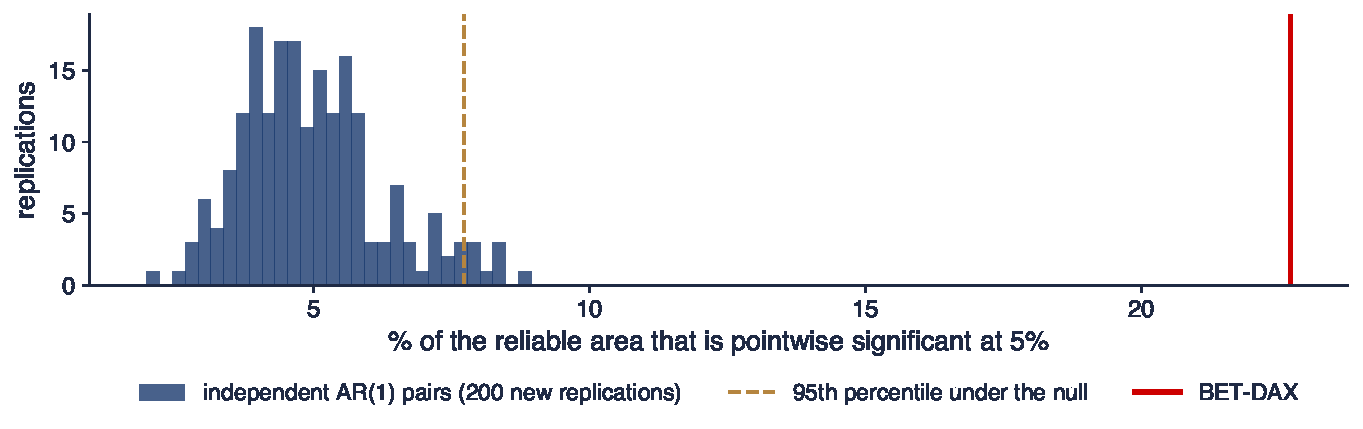
\includegraphics[width=0.97\textwidth,height=0.42\textheight,keepaspectratio]{ats_ch11_ai_case.pdf}
\end{center}
\vspace{-0.25cm}
\begin{itemize}
    \item Ponderea ariei timp--perioadă fiabile dintr-o hartă de coerență wavelet care este semnificativă punctual la 5\%: 200 de perechi noi de serii AR(1) independente, cu autocorelațiile BET și DAX, și harta observată BET--DAX
    \item Ipoteza nulă: media 5{,}0\%, percentila 95 7{,}7\%, maximum 9{,}0\%; 100\% din hărțile nule conțin insule semnificative; BET--DAX: 22{,}7\%. Un rezumat AI care citește fiecare insulă ca un episod de contagiune greșește; surplusul total este real
\end{itemize}
\quantlet{ATS\_ch11\_wavelet\_coherence}{\qlurl{ATS_ch11_wavelet_coherence}}
\end{frame}

\begin{frame}{Idee de proiect}
\itemsize{\small}
\begin{itemize}
    \item \textbf{Contagiune sau volatilitate? Coerența wavelet a piețelor bursiere din Europa Centrală și de Est sub o ipoteză nulă cu aceeași volatilitate}
    \begin{itemize}
        \item replicați: testul Monte Carlo al lui \refGMJ{} și hărțile de co-mișcare internațională ale lui \refRN{} pe BET, WIG20, BUX, PX față de DAX
        \item extindeți: o ipoteză nulă bootstrap dintr-un DCC-GARCH (dependență constantă, volatilitate variabilă); teste pe arii \refSch; coerență parțială controlînd pentru S\&P 500 \refACS
        \item preînregistrați: piețele, frecvența datelor, ferestrele de criză, scalele, modelul nul și numărul de replicări
    \end{itemize}
    \item Livrabilele urmează regulile cursului: repository, raport, AI\_USE.md, AI\_ERRORS.md, susținere orală
\end{itemize}
\end{frame}


%=============================================================================
\section{Încheiere}
%=============================================================================

\begin{frame}{Idei de reținut}
\itemsize{\small}
\begin{itemize}
    \item Spectrul descompune varianța pe frecvențe; filtrele acționează asupra lui prin pătratul cîștigului
    \item Estimarea este o alegere deplasare--varianță; multitaper dă scurgere mică, varianță stabilă și benzi corecte
    \item Coerența, faza, corelația dinamică și testele Breitung--Candelon descriu co-mișcarea și cauzalitatea pe frecvențe
    \item Un ciclu economic este ceea ce lasă să treacă cîștigul filtrului; HP adaugă cicluri false și eșuează în timp real
    \item Wavelets localizează varianța și co-mișcarea în timp și pe scale; semnificația cere Monte Carlo și o judecată pe arii
\end{itemize}
\end{frame}

\begin{frame}{Autoevaluare}
\itemsize{\small}
\begin{columns}[T]
\begin{column}{0.56\textwidth}
\begin{block}{Întrebări}
\begin{itemize}
    \item De ce este periodograma inconsistentă, deși este asimptotic nedeplasată?
    \item Cum crește lățimea de bandă optimă cu $n$ pentru un nucleu cu $q = 2$?
    \item De ce este coerența brută (nenetezită) întotdeauna egală cu unu?
    \item De unde provine vîrful ciclului HP al unui mers aleator?
    \item De ce este preferată MODWT față de DWT pentru varianța wavelet?
\end{itemize}
\end{block}
\end{column}
\begin{column}{0.40\textwidth}
\begin{block}{Urmează: \atschlink{https://danpele.github.io/Advanced-Time-Series/RO/Cursuri/capitol12_machine_learning_deep_learning.pdf}{Capitolul 12}}
\begin{itemize}
    \item Machine learning și deep learning pentru serii de timp
    \item modele globale, validare fără scurgere de informație, arhitecturi deep
\end{itemize}
\end{block}
\end{column}
\end{columns}
\end{frame}


%=============================================================================
\section{Anexă}
%=============================================================================

\begin{frame}{Anexă: distribuția periodogramei}
\itemsize{\small}
\begin{itemize}
    \item Zgomot alb gaussian: $a_j = \sqrt{2/n}\sum_tx_t\cos(\omega_jt)$, $b_j = \sqrt{2/n}\sum_tx_t\sin(\omega_jt)$ sînt i.i.d.\ $N(0, \sigma^2)$ pentru $0 < \omega_j < \pi$ (ortogonalitatea bazei Fourier)
    \item $I(\omega_j) = (a_j^2 + b_j^2)/(4\pi) = \frac{\sigma^2}{2\pi}\cdot\frac{\chi^2_2}{2}$: media $f = \sigma^2/(2\pi)$, varianța $f^2$, oricare ar fi $n$
    \item Proces liniar: $d_X(\omega_j) = \Psi(e^{-i\omega_j})d_\varepsilon(\omega_j) + o_p(1)$, deci $I_X(\omega_j) \approx |\Psi(e^{-i\omega_j})|^2I_\varepsilon(\omega_j) = f(\omega_j)\chi^2_2/2$
    \item Medierea a $L$ astfel de ordonate: media $f$, varianța $f^2/L$; aceasta este logica oricărui estimator netezit sau multitaper
\end{itemize}
\end{frame}

\begin{frame}{Anexă: două proprietăți ale filtrelor}
\itemsize{\small}
\begin{itemize}
    \item \textbf{Coerența este invariantă la filtrare}: $\tilde x = A(L)x$, $\tilde y = B(L)y$ dau $f_{\tilde x\tilde y} = A(\omega)\overline{B(\omega)}f_{xy}$, $f_{\tilde x} = |A|^2f_x$, $f_{\tilde y} = |B|^2f_y$, deci $\kappa^2_{\tilde x\tilde y} = \kappa^2_{xy}$ acolo unde $A, B \ne 0$
    \item Faza se schimbă cu $\arg A - \arg B$: o prealbire cu filtre diferite mută faza; folosiți același filtru pentru ambele serii
    \item \textbf{Ciclul HP al unui mers aleator}: $\Delta y = \varepsilon$, deci $f_c(\omega) = G(\omega)^2\sigma^2/(2\pi\cdot2(1 - \cos\omega))$; cu $u = 1 - \cos\omega$, aceasta este proporțională cu $u^3/(1 + 4\lambda u^2)^2$
    \item Anulînd derivata: $3(1 + 4\lambda u^2) = 16\lambda u^2$, deci $u^* = \sqrt{3/(4\lambda)}$, iar perioada este $2\pi/\arccos(1 - u^*)$
\end{itemize}
\end{frame}


%=============================================================================
\section{Bibliografie}
%=============================================================================

\begin{frame}{Bibliografie (1/3)}
\itemsize{\tiny}
\begin{itemize}
    \item Aguiar-Conraria, L., Azevedo, N., \& Soares, M. J. (2008). Using wavelets to decompose the time--frequency effects of monetary policy. \textit{Physica A}, 387(12), 2863--2878. \href{https://doi.org/10.1016/j.physa.2008.01.063}{doi:10.1016/j.physa.2008.01.063}
    \item Aguiar-Conraria, L., \& Soares, M. J. (2014). The continuous wavelet transform: Moving beyond uni- and bivariate analysis. \textit{Journal of Economic Surveys}, 28(2), 344--375. \href{https://doi.org/10.1111/joes.12012}{doi:10.1111/joes.12012}
    \item Andrews, D. W. K. (1991). Heteroskedasticity and autocorrelation consistent covariance matrix estimation. \textit{Econometrica}, 59(3), 817--858. \href{https://doi.org/10.2307/2938229}{doi:10.2307/2938229}
    \item Baxter, M., \& King, R. G. (1999). Measuring business cycles: Approximate band-pass filters for economic time series. \textit{Review of Economics and Statistics}, 81(4), 575--593. \href{https://doi.org/10.1162/003465399558454}{doi:10.1162/003465399558454}
    \item Breitung, J., \& Candelon, B. (2006). Testing for short- and long-run causality: A frequency-domain approach. \textit{Journal of Econometrics}, 132(2), 363--378. \href{https://doi.org/10.1016/j.jeconom.2005.02.004}{doi:10.1016/j.jeconom.2005.02.004}
    \item Brockwell, P. J., \& Davis, R. A. (1991). \textit{Time Series: Theory and Methods} (2nd ed.). Springer. \href{https://doi.org/10.1007/978-1-4419-0320-4}{doi:10.1007/978-1-4419-0320-4}
    \item Christiano, L. J., \& Fitzgerald, T. J. (2003). The band pass filter. \textit{International Economic Review}, 44(2), 435--465. \href{https://doi.org/10.1111/1468-2354.t01-1-00076}{doi:10.1111/1468-2354.t01-1-00076}
    \item Cogley, T., \& Nason, J. M. (1995). Effects of the Hodrick--Prescott filter on trend and difference stationary time series: Implications for business cycle research. \textit{Journal of Economic Dynamics and Control}, 19(1--2), 253--278. \href{https://doi.org/10.1016/0165-1889(93)00781-X}{doi:10.1016/0165-1889(93)00781-X}
    \item Croux, C., Forni, M., \& Reichlin, L. (2001). A measure of comovement for economic variables: Theory and empirics. \textit{Review of Economics and Statistics}, 83(2), 232--241. \href{https://doi.org/10.1162/00346530151143770}{doi:10.1162/00346530151143770}
    \item Crowley, P. M. (2007). A guide to wavelets for economists. \textit{Journal of Economic Surveys}, 21(2), 207--267. \href{https://doi.org/10.1111/j.1467-6419.2006.00502.x}{doi:10.1111/j.1467-6419.2006.00502.x}
    \item Dahlhaus, R. (1997). Fitting time series models to nonstationary processes. \textit{The Annals of Statistics}, 25(1), 1--37. \href{https://doi.org/10.1214/aos/1034276620}{doi:10.1214/aos/1034276620}
    \item Daubechies, I. (1988). Orthonormal bases of compactly supported wavelets. \textit{Communications on Pure and Applied Mathematics}, 41(7), 909--996. \href{https://doi.org/10.1002/cpa.3160410705}{doi:10.1002/cpa.3160410705}
    \item Fidrmuc, J., \& Korhonen, I. (2006). Meta-analysis of the business cycle correlation between the euro area and the CEECs. \textit{Journal of Comparative Economics}, 34(3), 518--537. \href{https://doi.org/10.1016/j.jce.2006.06.007}{doi:10.1016/j.jce.2006.06.007}
    \item Forbes, K. J., \& Rigobon, R. (2002). No contagion, only interdependence: Measuring stock market comovements. \textit{The Journal of Finance}, 57(5), 2223--2261. \href{https://doi.org/10.1111/0022-1082.00494}{doi:10.1111/0022-1082.00494}
    \item Gençay, R., Selçuk, F., \& Whitcher, B. (2005). Multiscale systematic risk. \textit{Journal of International Money and Finance}, 24(1), 55--70. \href{https://doi.org/10.1016/j.jimonfin.2004.10.003}{doi:10.1016/j.jimonfin.2004.10.003}
    \item Gençay, R., Selçuk, F., \& Whitcher, B. (2002). Wavelets for variance--covariance estimation. In \textit{An Introduction to Wavelets and Other Filtering Methods in Finance and Economics}. Academic Press. \href{https://doi.org/10.1016/B978-012279670-8.50010-0}{doi:10.1016/B978-012279670-8.50010-0}
\end{itemize}
\end{frame}

\begin{frame}{Bibliografie (2/3)}
\itemsize{\tiny}
\begin{itemize}
    \item Geweke, J. (1982). Measurement of linear dependence and feedback between multiple time series. \textit{Journal of the American Statistical Association}, 77(378), 304--313. \href{https://doi.org/10.1080/01621459.1982.10477803}{doi:10.1080/01621459.1982.10477803}
    \item Granger, C. W. J. (1966). The typical spectral shape of an economic variable. \textit{Econometrica}, 34(1), 150--161. \href{https://doi.org/10.2307/1909859}{doi:10.2307/1909859}
    \item Grinsted, A., Moore, J. C., \& Jevrejeva, S. (2004). Application of the cross wavelet transform and wavelet coherence to geophysical time series. \textit{Nonlinear Processes in Geophysics}, 11(5/6), 561--566. \href{https://doi.org/10.5194/npg-11-561-2004}{doi:10.5194/npg-11-561-2004}
    \item Grossmann, A., \& Morlet, J. (1984). Decomposition of Hardy functions into square integrable wavelets of constant shape. \textit{SIAM Journal on Mathematical Analysis}, 15(4), 723--736. \href{https://doi.org/10.1137/0515056}{doi:10.1137/0515056}
    \item Hamilton, J. D. (2018). Why you should never use the Hodrick--Prescott filter. \textit{The Review of Economics and Statistics}, 100(5), 831--843. \href{https://doi.org/10.1162/rest_a_00706}{doi:10.1162/rest\_a\_00706}
    \item Harding, D., \& Pagan, A. (2002). Dissecting the cycle: A methodological investigation. \textit{Journal of Monetary Economics}, 49(2), 365--381. \href{https://doi.org/10.1016/S0304-3932(01)00108-8}{doi:10.1016/S0304-3932(01)00108-8}
    \item Hodrick, R. J., \& Prescott, E. C. (1997). Postwar U.S. business cycles: An empirical investigation. \textit{Journal of Money, Credit and Banking}, 29(1), 1--16. \href{https://doi.org/10.2307/2953682}{doi:10.2307/2953682}
    \item Hurvich, C. M. (1985). Data-driven choice of a spectrum estimate: Extending the applicability of cross-validation methods. \textit{Journal of the American Statistical Association}, 80(392), 933--940. \href{https://doi.org/10.1080/01621459.1985.10478207}{doi:10.1080/01621459.1985.10478207}
    \item Kilian, L., \& Park, C. (2009). The impact of oil price shocks on the U.S. stock market. \textit{International Economic Review}, 50(4), 1267--1287. \href{https://doi.org/10.1111/j.1468-2354.2009.00568.x}{doi:10.1111/j.1468-2354.2009.00568.x}
    \item Liu, Y., San Liang, X., \& Weisberg, R. H. (2007). Rectification of the bias in the wavelet power spectrum. \textit{Journal of Atmospheric and Oceanic Technology}, 24(12), 2093--2102. \href{https://doi.org/10.1175/2007JTECHO511.1}{doi:10.1175/2007JTECHO511.1}
    \item Mallat, S. G. (1989). A theory for multiresolution signal decomposition: The wavelet representation. \textit{IEEE Transactions on Pattern Analysis and Machine Intelligence}, 11(7), 674--693. \href{https://doi.org/10.1109/34.192463}{doi:10.1109/34.192463}
    \item Maraun, D., \& Kurths, J. (2004). Cross wavelet analysis: Significance testing and pitfalls. \textit{Nonlinear Processes in Geophysics}, 11(4), 505--514. \href{https://doi.org/10.5194/npg-11-505-2004}{doi:10.5194/npg-11-505-2004}
    \item Parzen, E. (1961). Mathematical considerations in the estimation of spectra. \textit{Technometrics}, 3(2), 167--190. \href{https://doi.org/10.1080/00401706.1961.10489939}{doi:10.1080/00401706.1961.10489939}
    \item Percival, D. B. (1995). On estimation of the wavelet variance. \textit{Biometrika}, 82(3), 619--631. \href{https://doi.org/10.1093/biomet/82.3.619}{doi:10.1093/biomet/82.3.619}
    \item Percival, D. B., \& Walden, A. T. (1993). \textit{Spectral Analysis for Physical Applications: Multitaper and Conventional Univariate Techniques}. Cambridge University Press. \href{https://doi.org/10.1017/CBO9780511622762}{doi:10.1017/CBO9780511622762}
    \item Percival, D. B., \& Walden, A. T. (2000). \textit{Wavelet Methods for Time Series Analysis}. Cambridge University Press. \href{https://doi.org/10.1017/CBO9780511841040}{doi:10.1017/CBO9780511841040}
\end{itemize}
\end{frame}

\begin{frame}{Bibliografie (3/3)}
\itemsize{\tiny}
\begin{itemize}
    \item Petropoulos, F., Apiletti, D., Assimakopoulos, V., Babai, M. Z., et al.\ (2022). Forecasting: Theory and practice. \textit{International Journal of Forecasting}, 38(3), 705--871. \href{https://doi.org/10.1016/j.ijforecast.2021.11.001}{doi:10.1016/j.ijforecast.2021.11.001}
    \item Phillips, P. C. B., \& Shi, Z. (2021). Boosting: Why you can use the HP filter. \textit{International Economic Review}, 62(2), 521--570. \href{https://doi.org/10.1111/iere.12495}{doi:10.1111/iere.12495}
    \item Priestley, M. B. (1965). Evolutionary spectra and non-stationary processes. \textit{Journal of the Royal Statistical Society: Series B}, 27(2), 204--229. \href{https://doi.org/10.1111/j.2517-6161.1965.tb01488.x}{doi:10.1111/j.2517-6161.1965.tb01488.x}
    \item Quast, J., \& Wolters, M. H. (2022). Reliable real-time output gap estimates based on a modified Hamilton filter. \textit{Journal of Business \& Economic Statistics}, 40(1), 152--168. \href{https://doi.org/10.1080/07350015.2020.1784747}{doi:10.1080/07350015.2020.1784747}
    \item Ravn, M. O., \& Uhlig, H. (2002). On adjusting the Hodrick--Prescott filter for the frequency of observations. \textit{Review of Economics and Statistics}, 84(2), 371--376. \href{https://doi.org/10.1162/003465302317411604}{doi:10.1162/003465302317411604}
    \item Riedel, K. S., \& Sidorenko, A. (1995). Minimum bias multiple taper spectral estimation. \textit{IEEE Transactions on Signal Processing}, 43(1), 188--195. \href{https://doi.org/10.1109/78.365298}{doi:10.1109/78.365298}
    \item Rua, A., \& Nunes, L. C. (2009). International comovement of stock market returns: A wavelet analysis. \textit{Journal of Empirical Finance}, 16(4), 632--639. \href{https://doi.org/10.1016/j.jempfin.2009.02.002}{doi:10.1016/j.jempfin.2009.02.002}
    \item Schulte, J. A. (2016). Cumulative areawise testing in wavelet analysis and its application to geophysical time series. \textit{Nonlinear Processes in Geophysics}, 23(1), 45--57. \href{https://doi.org/10.5194/npg-23-45-2016}{doi:10.5194/npg-23-45-2016}
    \item Shumway, R. H., \& Stoffer, D. S. (2017). \textit{Time Series Analysis and Its Applications: With R Examples} (4th ed.). Springer. \href{https://doi.org/10.1007/978-3-319-52452-8}{doi:10.1007/978-3-319-52452-8}
    \item Thomson, D. J. (1982). Spectrum estimation and harmonic analysis. \textit{Proceedings of the IEEE}, 70(9), 1055--1096. \href{https://doi.org/10.1109/PROC.1982.12433}{doi:10.1109/PROC.1982.12433}
    \item Torrence, C., \& Compo, G. P. (1998). A practical guide to wavelet analysis. \textit{Bulletin of the American Meteorological Society}, 79(1), 61--78. \href{https://doi.org/10.1175/1520-0477(1998)079\%3C0061:APGTWA\%3E2.0.CO;2}{doi:10.1175/1520-0477(1998)079\textless{}0061:APGTWA\textgreater{}2.0.CO;2}
    \item Torrence, C., \& Webster, P. J. (1999). Interdecadal changes in the ENSO--monsoon system. \textit{Journal of Climate}, 12(8), 2679--2690. \href{https://doi.org/10.1175/1520-0442(1999)012\%3C2679:ICITEM\%3E2.0.CO;2}{doi:10.1175/1520-0442(1999)012\textless{}2679:ICITEM\textgreater{}2.0.CO;2}
    \item Vacha, L., \& Barunik, J. (2012). Co-movement of energy commodities revisited: Evidence from wavelet coherence analysis. \textit{Energy Economics}, 34(1), 241--247. \href{https://doi.org/10.1016/j.eneco.2011.10.007}{doi:10.1016/j.eneco.2011.10.007}
    \item Vautard, R., \& Ghil, M. (1989). Singular spectrum analysis in nonlinear dynamics, with applications to paleoclimatic time series. \textit{Physica D}, 35(3), 395--424. \href{https://doi.org/10.1016/0167-2789(89)90077-8}{doi:10.1016/0167-2789(89)90077-8}
    \item Welch, P. D. (1967). The use of fast Fourier transform for the estimation of power spectra: A method based on time averaging over short, modified periodograms. \textit{IEEE Transactions on Audio and Electroacoustics}, 15(2), 70--73. \href{https://doi.org/10.1109/TAU.1967.1161901}{doi:10.1109/TAU.1967.1161901}
    \item Whitcher, B., Guttorp, P., \& Percival, D. B. (2000). Wavelet analysis of covariance with application to atmospheric time series. \textit{Journal of Geophysical Research: Atmospheres}, 105(D11), 14941--14962. \href{https://doi.org/10.1029/2000JD900110}{doi:10.1029/2000JD900110}
\end{itemize}
\end{frame}

\end{document}
